\chapter[Evaluation of Cloud Cuts on Auger Event Data]{\centering Evaluation of Cloud Cuts on Auger Event Data \\}\label{Ch:CloudCuts}

First look into the effectiveness of the Cloud cuts on Auger Golden Hybrid data from 2004 to 2018.
I investigated the effects of removing the cloud cut from the list of quality cuts. This list includes cuts to remove events within known bad data taking periods, cuts on aerosol levels, event quality etc. Within the method section I shown an example of a cuts file that is used within Auger.

This investigation was done to quantify the effects that the cloud cuts had on the data set. A question had been raised about whether the quality cuts on fitted values, Chi2 and requiring events with large gaps where doing the same job as the cloud cuts. There is a lot of uncertainty about whether a detected cloud had impacted each events.

It is important to know where clouds are located in relation to EAS events due to the different effects that clouds can have on the detected light profile by the FDs. If a cloud partially obscures the FD view of the event it can causing a gap in the profile or a cloud may in the path of the development of the EAS event. In the first case a gap will cause the reconstruction of the energy of the event to be underestimated. While in the second case a cloud within the path of development can amplify the amount of Cherenkov light scattered towards the FD which can in turn cause an overestimate of the reconstructed energy.

Cloud information has large uncertainty about quantities like cloud height, distance from telescopes and timing. The timing uncertainty is due to atmospheric data being snapshots with time gaps between shots. Examples are Cloud camera scans are performed every 5 minutes. A cloud could move quite a far distance within this time.

\section{Equipment used to monitor clouds above the array}

There are multiple instruments used to monitor the cloud coverage across the array. These are a combination of collaboration run instruments specifically setup to monitor atmospheric conditions within the array and externally run instruments that monitor boarder atmospheric conditions that happen to include the array. 

The combination of instruments used to monitor clouds are the bistatic lidar system, the Geostationary Operational Environmental Satellite (GOES) system, Infra-red cameras and the Central Laser Facility (CLF).

\begin{figure}
\begin{subfigure}[b]{0.3\textwidth}
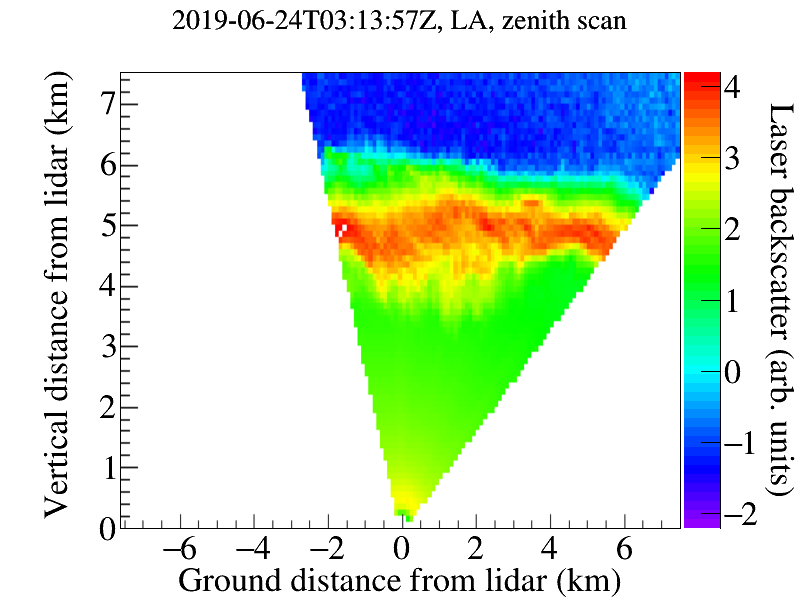
\includegraphics[width=\textwidth]{chapters/graphs/CloudFlags/lidar_scan.png}
\caption{} \label{subfig:liadr_scan}
\end{subfigure}
\begin{subfigure}[b]{0.3\textwidth}
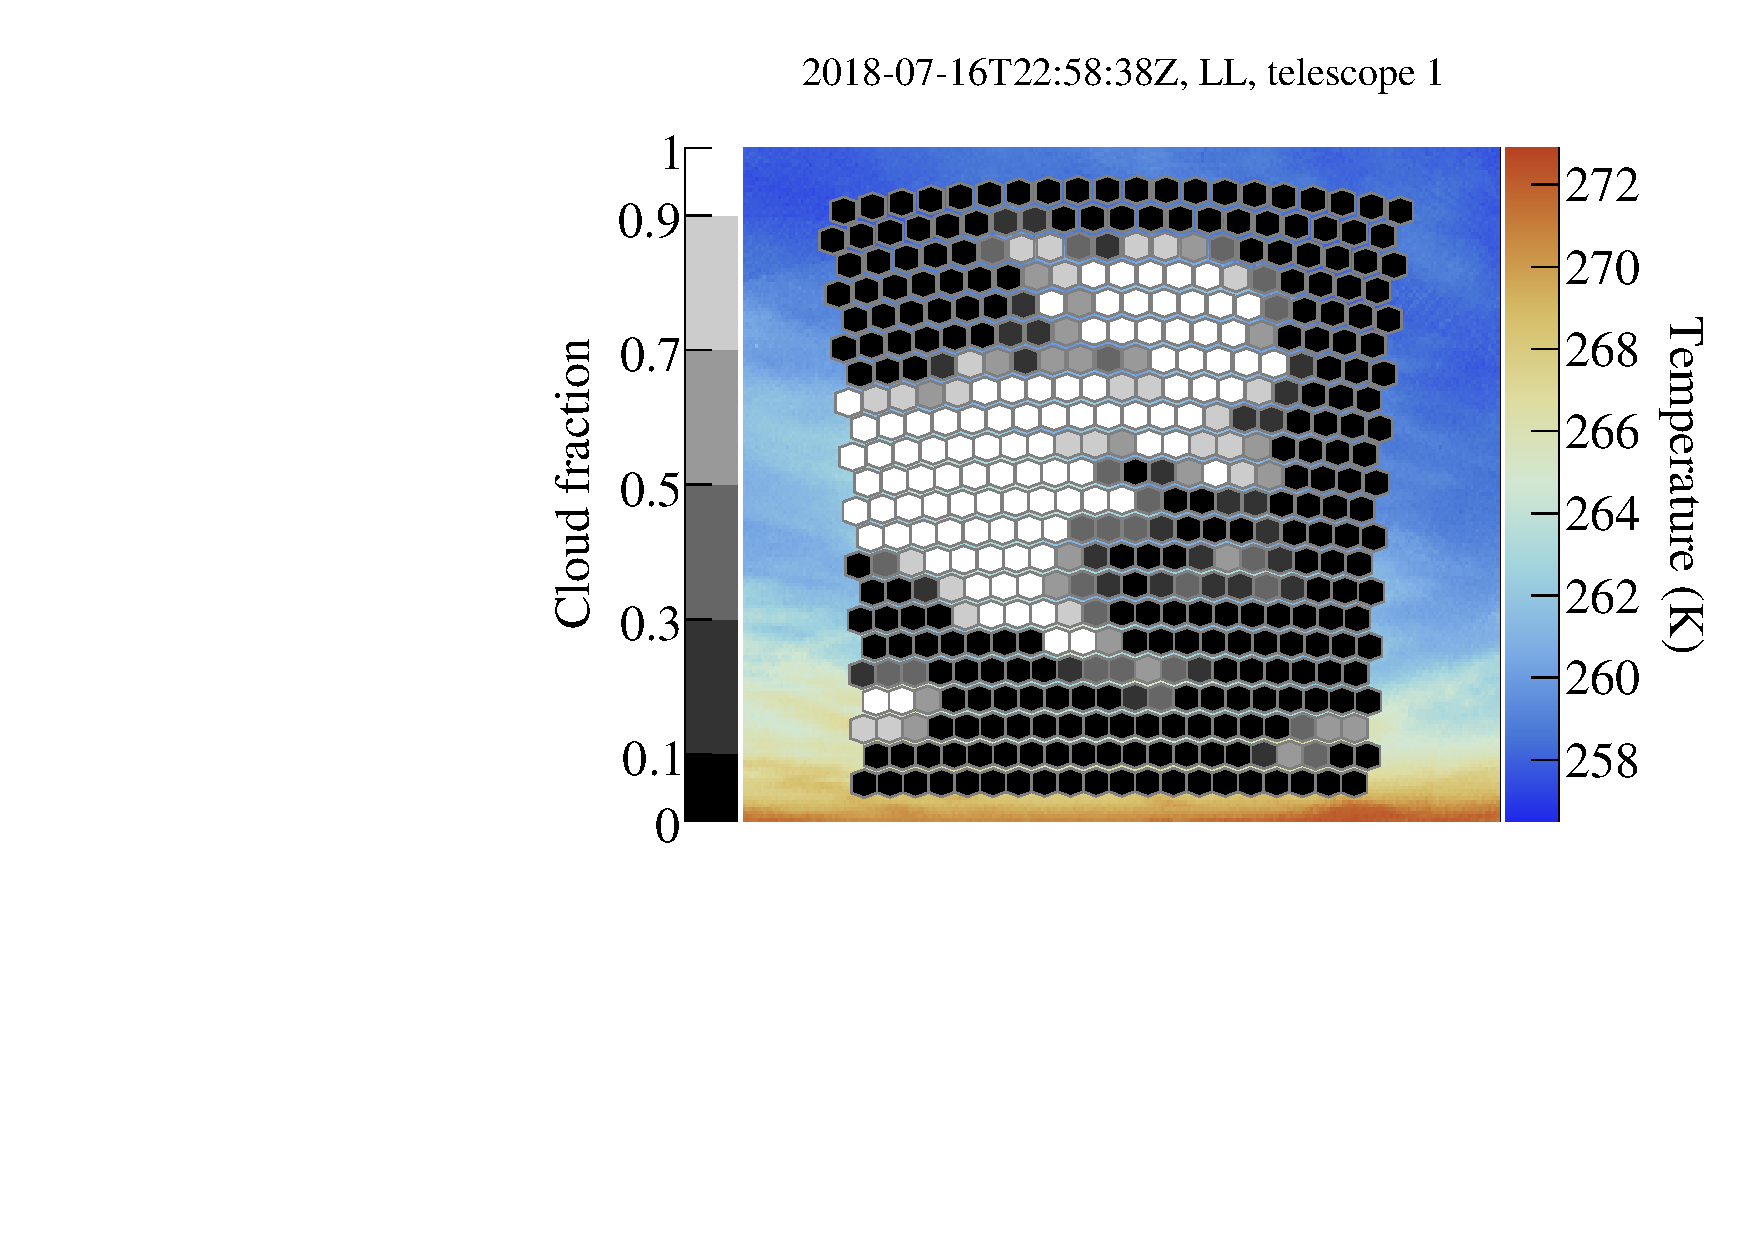
\includegraphics[width=\textwidth]{chapters/graphs/CloudFlags/ir_cloudfraction_pixels.pdf}
\caption{} \label{subfig:IR_cloudcam}
\end{subfigure}
\begin{subfigure}[b]{0.3\textwidth}
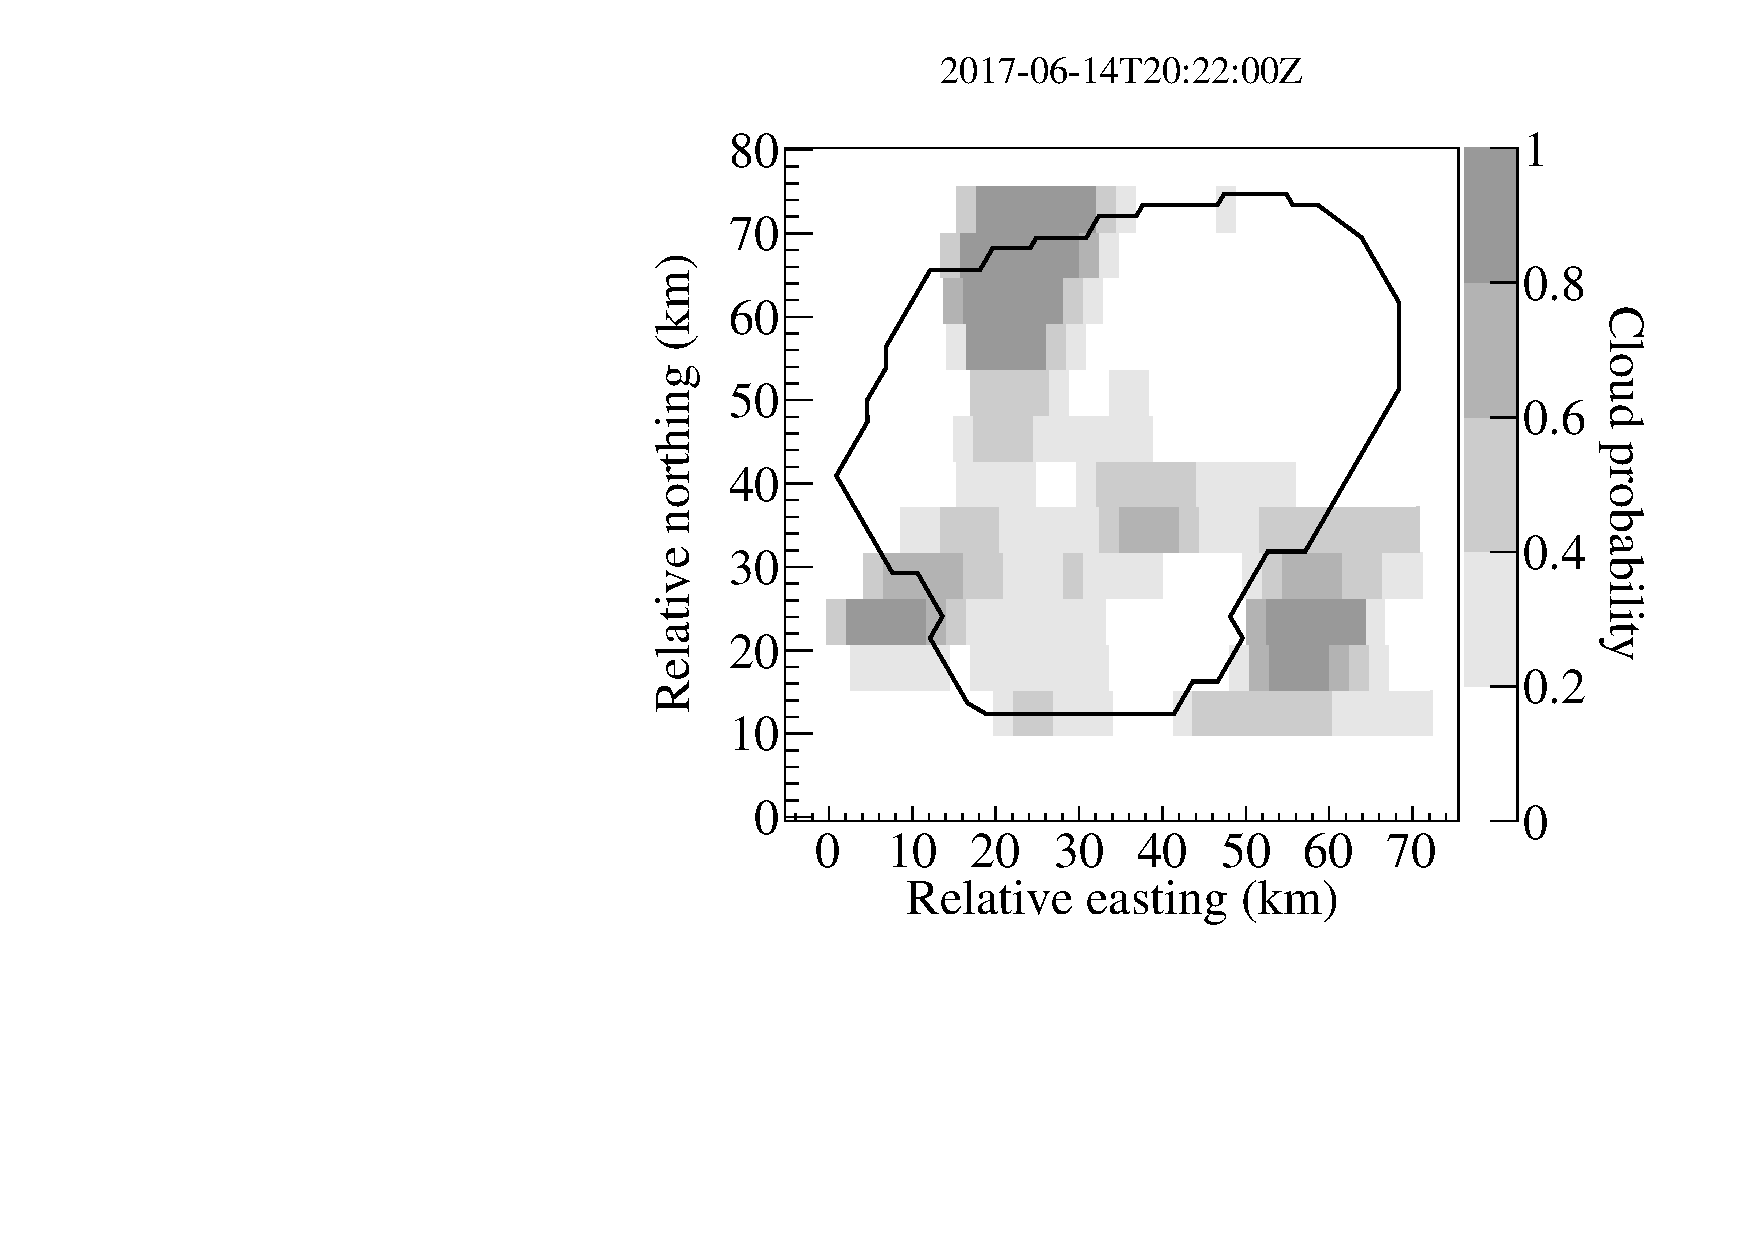
\includegraphics[width=\textwidth]{chapters/graphs/CloudFlags/ir_cloudprobability_map.pdf}
\caption{} \label{subfig:GOES}
\end{subfigure}
\caption{Examples of real data from (a) FD lidar scan, (b) cloud camera mask mapped to each pixel of a single FD telescope and (c) GOES cloud probability map covering the entire array.  Images provide by permission by V. Harvey.}
\end{figure}

 
\subsection{Bistatic Lidar System}

A monostatic elastic backscatter lidar is deployed behind each of the FD telescope sites and is programmed to scan the sky above the FD field of view every 15 minutes. The lidar is primarily used to monitor aerosols but has the secondary benefit of detecting clouds. it works on the principle of measuring the time delay and magnitude of the returned signal to determine the distance and density of scattering centres. Both a minimum cloud base height (CBH) and percentage of overhead cloud coverage can be calculated. The overall CBH is an hourly average of all the 15 minute scans from all the FD sites. An example of a returned signal map is shown in Figure \ref{subfig:liadr_scan}. This example shows that an overhead scan which indicates a localised cloud base height (CBH) of 4 km. The CBH and percentage of overhead cloud coverage is used when considering whether an event can used in different analyses within Auger.  

- need to talk about both the lidars at each FD sites and the CLF/XLF
- information at FD sites, above the CLF/XLF and between the XLF/CLF and FD telescopes that see these lasers.



\subsection{Infra-Red Cameras}

The main way clouds are monitored is by infra-red cameras located on the roof of each FD eyes. The cameras record light between 8 $\mu$m and 14 $\mu$m which measurement clouds as warmer then the sky. The cloud cameras take images with the FoV of the FD eyes every 5 minutes while a full sky scan is performed every 15 minutes. The images within the FoV of the FD eyes are analysed to calculate a cloud fraction between 0\% and 100\% for each FD pixel. An example of the cloud mask being map to individual FD pixels is shown in Figure \ref{subfig:IR_cloudcam}. The pixels observing $\sim$ 5\textdegree \ above the horizon and below are not assigned a cloud fraction as observing clouds this close to the ground is difficult. The difficulty arise due to the fact that in IR the atmosphere becomes optically thick close to the horizon and the large present of water vapour close to the ground. When an event is reconstructed, the cloud fraction of each FD pixel that observed the EAS event is queried.

\subsection{Geostationary Operational Environmental Satellite (GOES) system}

The Geostationary Operational Environmental Satellite system (GOES) is operated by the United States National Oceanic and Atmospheric Administration. Auger uses the raw data that is publicly available and has created an algorithm to convert the aerial measurements across four IR bands to produce a cloud probability map every 30 minutes. An example of an GOES cloud probability map is shown in Figure \ref{subfig:GOES}. Each block represents a satellite pixel that covers an 2.4 km by 5.5 km area on the ground.

\section{Cloud Cuts employed on Auger data}

Event passes clouds cut through a series of levels. The first check starts at (a) as go through to  If an event passes a cut no further checks are performed.

\begin{itemize}
\item[(a)] If IR Cloud Mask is available for the pixels involved, an event will pass if there's 0\% cloud fraction. The cloud fraction is not calculated for pixel below 5.5\textdegree. 
\item[(b)] Similar to step (a) if FD lidar is available can use the nearest FD lidar to determine the CBH to help whether the cloud is in front or behind the shower. An event will pass if the targeted cloud fration is 0\%.
\item[(c)] If GOES data is available check the satellite pixels to calculate the cloud probability between the FD site and the observed shower axis. If the cloud probability alone the between is 0\% then the event will pass.
\item[(d)] If i write something here what happens
\begin{itemize}
\item[(1)]
\item[(2)]
\end{itemize}
\item[(e)]
\end{itemize}

\begin{figure}
\centering
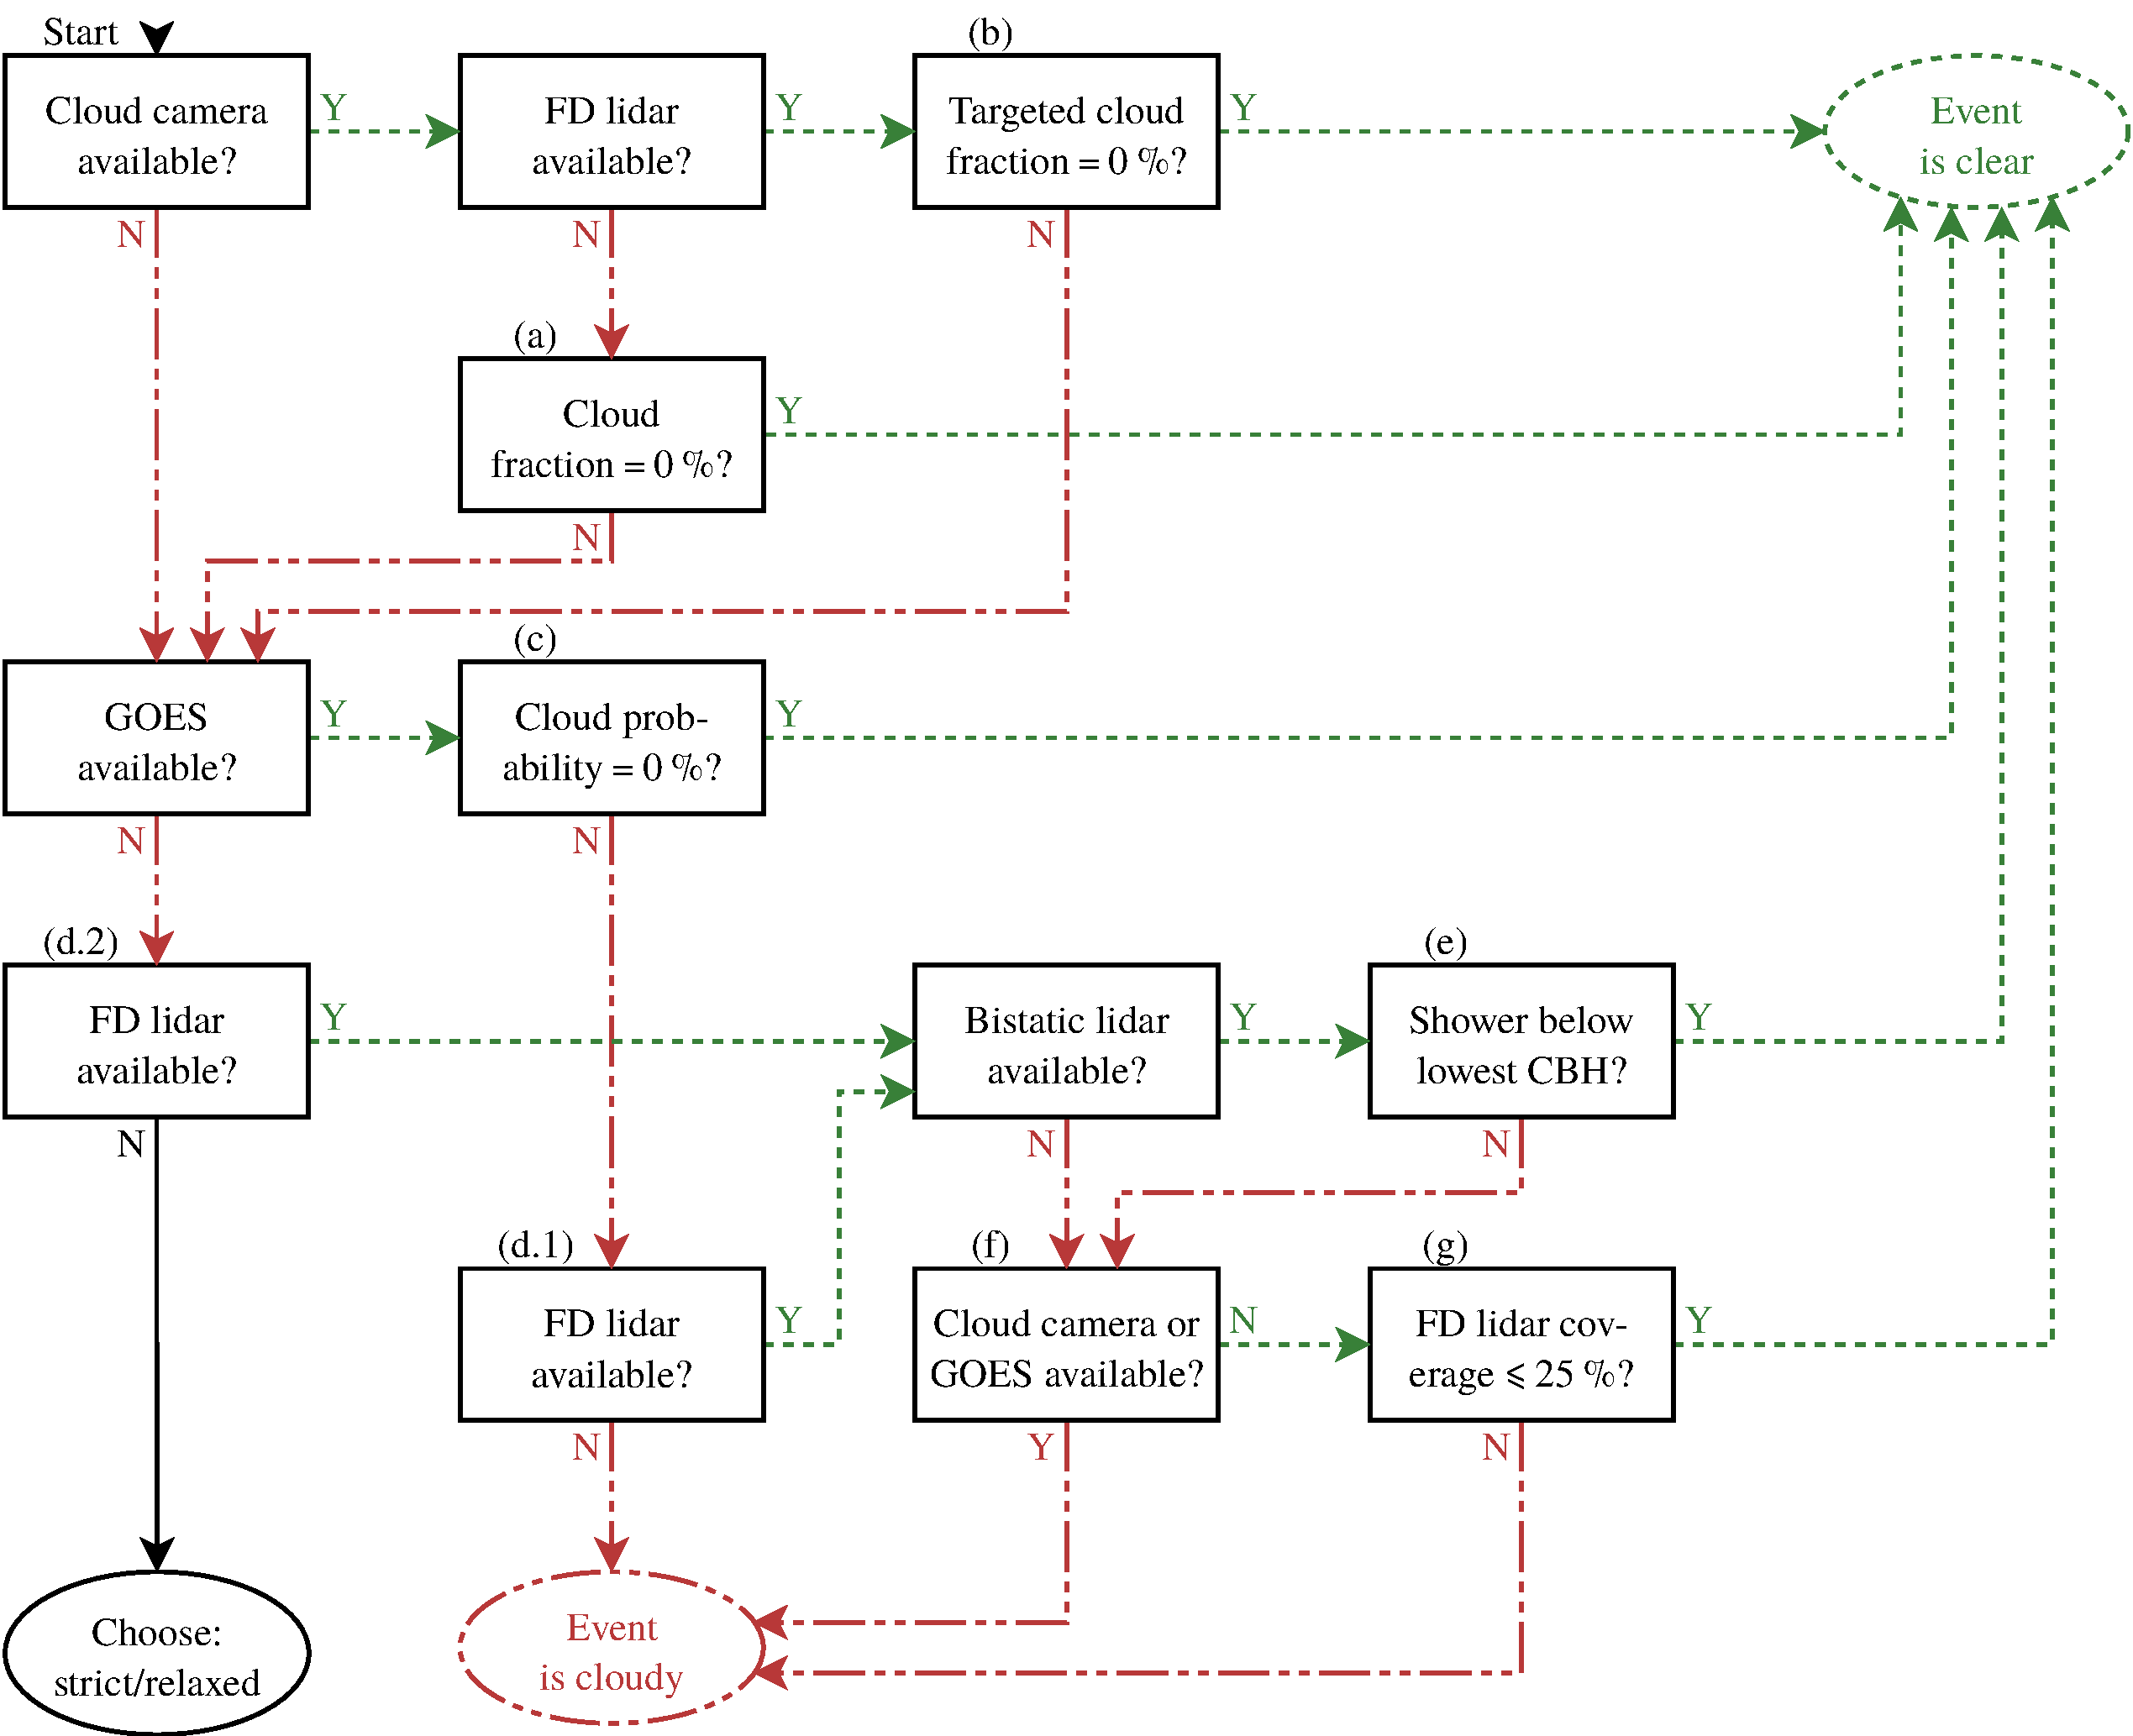
\includegraphics[width=0.7\textwidth]{chapters/graphs/CloudFlags/cloud_cuts.pdf}
\caption{Diagram of how the cloud cuts are applied to the data set when called with the Auger event selection program. Image provide by permission by V. Harvey}
\end{figure}

\section{Cloud Flags Investigation Method}

%Take reconstructed Golden Hybrid events from 2004 to 2018 
%
%Extract camera flag data.
%
%Two set of camera flags - positive ones that say that an event has pass one of the conditions saying that these is no cloud. the negative flags say that the event has failed to pass any of the test looking for clouds. If the flag is zero then there is no cloud information available.
%
%Four different flags - IR Cloud camera, LIDAR, GOES satellite data and something else.
%
%Look at the histograms of Xmax distributions for data passing cloud cuts, data failing cloud cuts and combined.

The method to investigate the effects of the cloud cuts on the Auger data was applied to the Golden Hybrid data set with events from 2004 to 2018. First the events are reconstructed through the Auger OffLine program and then the reconstructed events are passed through a selectEvents program. This selectEvents program utilises a series of parameters to apply quality cuts to the reconstructed events. The list of cuts used are shown in Tab \ref{}. The cuts used on the data set where the ICRC2019 list of cuts taken from within the collaboration OffLine application.

Event selected for the analysis based on the quality cuts used for the 2019 ICRC data set. All of the cuts were applied expect for the Cloud Cuts. I then took the code that would assign the cloud flag to an event and then used it within my own analysis code. The code was then used to apply a flag number to indicate which of the cloud cuts the event would pass or fail.

I assigned a positive value between 1 and 5 to say that the event was cloud free. The number indicates which monitoring instrument said that there was no clouds between the event and the triggered Fluorescence Telescope (FD). A zero meant that there was no data from any monitoring instrument. A negative number was used to denote that a monitoring instrument had seen clouds that have a high probability of impacting the event seen by the triggered  FD.

From there I looked into Elongation Rate (Xmax vs log$_{10}$(Energy)) which is of concern for any study involving mass composition. I also show the distributions of events in log$_{10}$(Energy) and Xmax. The Xmax plots are split up into different energy bins to see the distributions. I was particularly interested in qualifying the tails of these distributions as they would of most concern to any mass composition analysis. This analysis needs to have confidence in the calculation of the mean and standard deviation which used to indicate the average composition of events within a particular energy bin. 

I also show examples of individual events that would and would not pass the cloud cuts. This is to give a visual indication of what events that would pass look like and compare this to events that would fail the cloud cut. I have also shown some events that have weird properties which I will explain further within the results and discussion section.


\section{Results - Effect on Mean Xmax and Spread in Xmax}

%- Cloud Cut Flags distribution
%
%- Xmax distributions within energy bins
%
%- Elongation rate  
%
%- Is distance to Xmax or distance to shower axis needed?

\subsection{Cloud Flags Distribution}

Figure \ref{fig:cloudFlag_dist} shows the distribution of reconstruction shower events that would pass all quality cuts what Cloud Cut Flag has been assigned to them. Greater than zero means that the event has passed one of the cases to say that the event has a high probability it has not been effected by clouds. Less than zero means that the event has had a cloud detected close enough in space or time with a high probability to have had an effect. Zero means that there is not definite measurement that the event has or has not been effected by clouds. Events with the zero flag are kept or discarded whether the loose or strict settings are used. In this case the loose setting was used so the events with flag equal to zero were marked as considered to not having any cloud.

\subsection{Elongation Rate}

Figure \ref{fig:ElongRate_hist} shows how the elongation rate as a function of energy. Within this figure shows the mean and standard deviation of the Xmax within each energy bin. The standard deviation is shown as it is of importance to mass composition studies. There is no significance difference between the elongation  rates of the different data sets with Cloud Cuts applied (blue downwards triangles), without any Cloud Cuts (black squares) and only events that would fail the cloud cuts (red upward triangles).

\begin{figure}
\centering
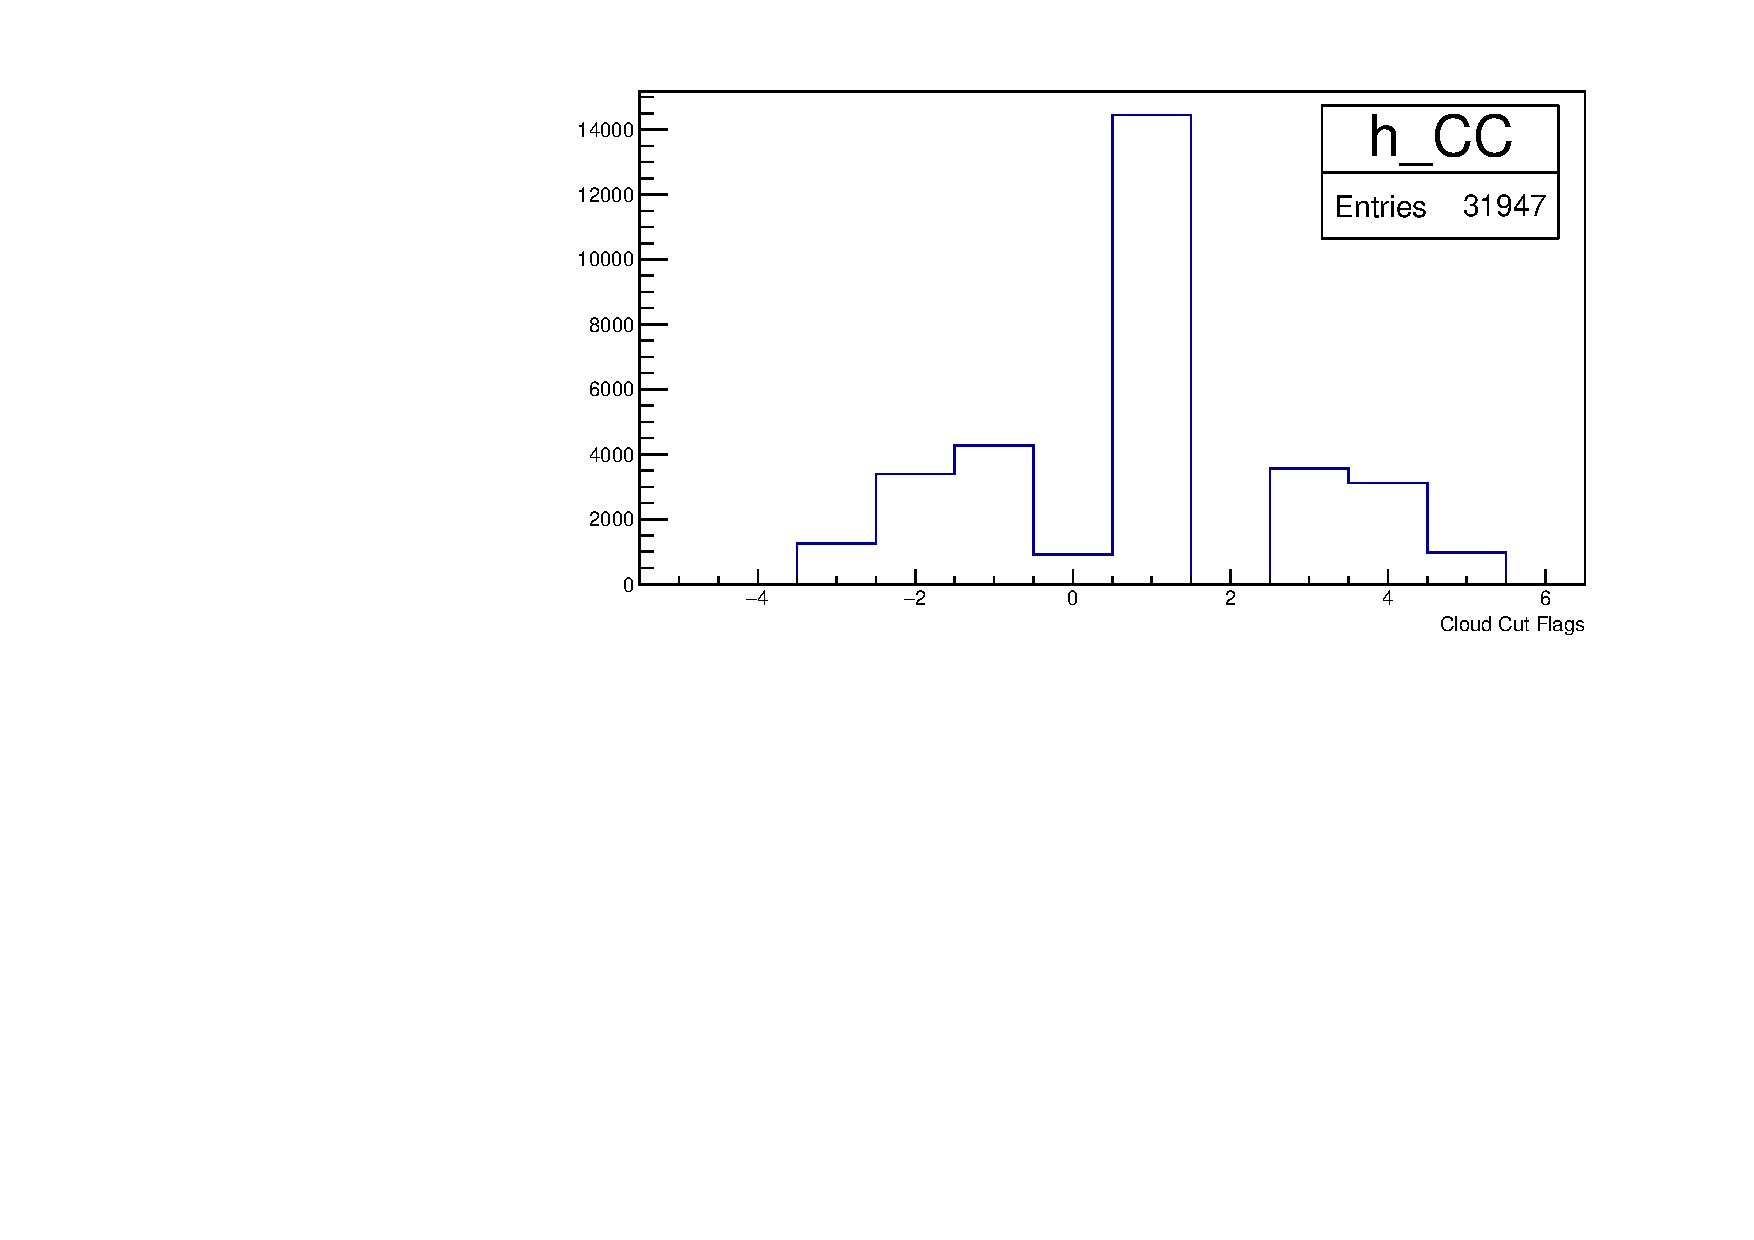
\includegraphics[width=\textwidth]{chapters/graphs/CloudFlags/hist_cloudFlags.pdf}
\caption{Distribution of cloud flags. Positive flag values are for events that would pass one of the cloud cuts. Negative flag values are for events that would fail one of the cloud cuts. A flag value of zero is for events that have no cloud data.}\label{fig:cloudFlag_dist}
\end{figure}

\begin{figure}
\centering
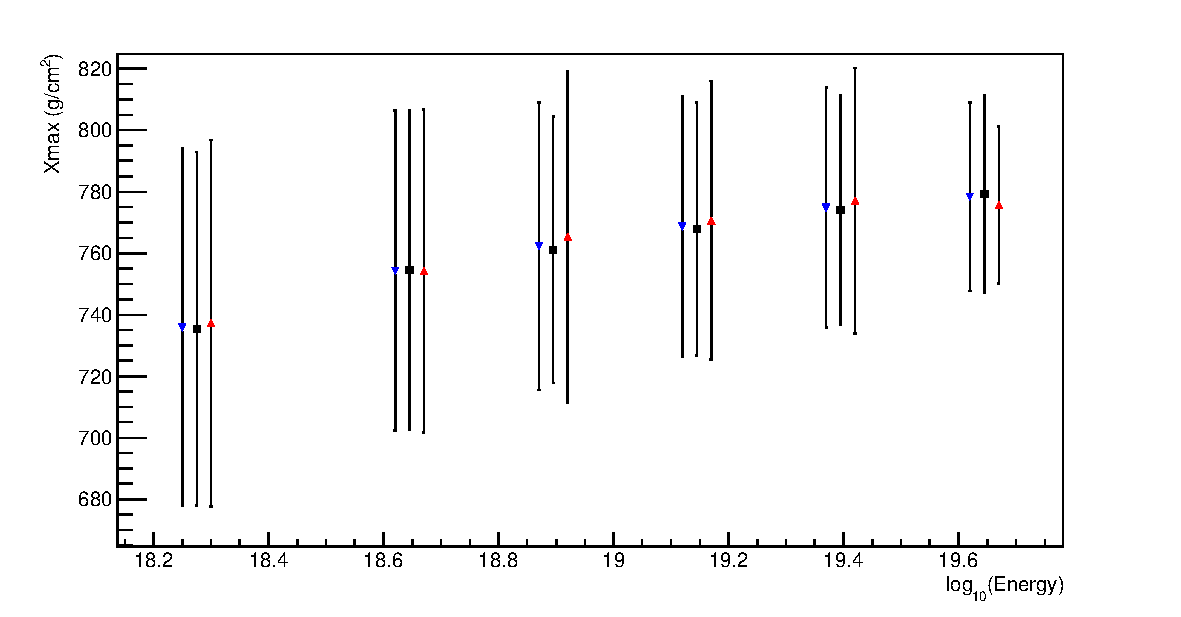
\includegraphics[width=\textwidth]{chapters/graphs/CloudFlags/ElongationRate.pdf}
\caption{Elongation Rate with Cloud cuts applied (blue downward triangle), without any cloud cuts (black square) and only events that would fail the cloud cuts (red upward triangle).} \label{fig:ElongRate_hist}
\end{figure}

% Energy Distribution

\subsection{Spectrum of events by Energy}

Comparison distributions of the energy spectrum observed by Auger. The events are selected, after being successfully reconstructed, by passing through a series of quality cuts. The comparison is done on data sets that contain events that only pass the cloud cut, only fail the cloud cut and a data set whether the cloud cut is removed. Figure \ref{fig:cloudFlag_energyDist} shows the number events per energy bin above 10$^{18}$ eV. The distribution shows the how the shape of the distribution is not effected by whether clouds are present or not. This is a good sign as clouds should not preferentially block events at any particular energy. The only different is the total number of events in each energy bin.

\begin{figure}
\centering
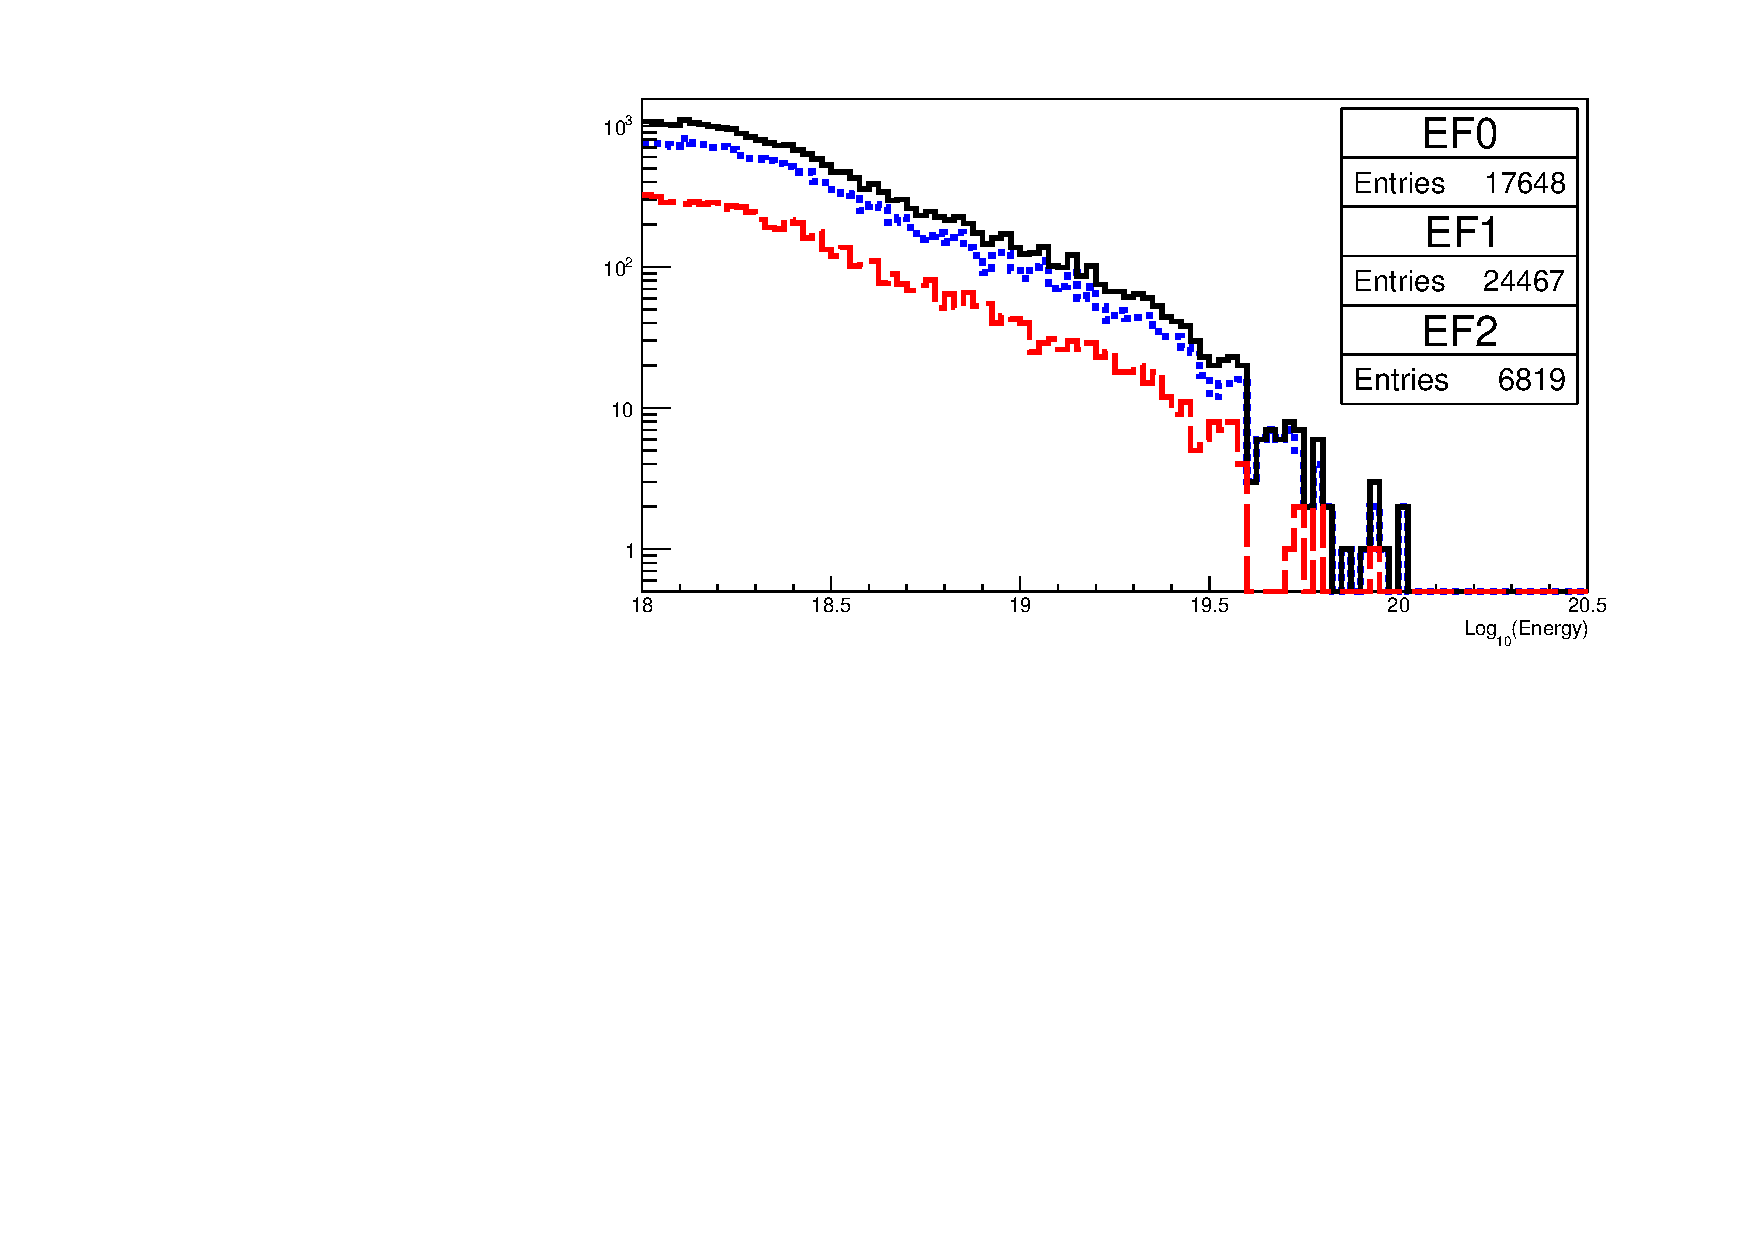
\includegraphics[width=\textwidth]{/home/tsudholz/PhD/Thesis/chapters/graphs/CloudFlags/EnergyHistAll_logE_18_0to20_5_Comb2.pdf}
\caption{Distribution of the energy of events within the bin of log(E) of 18.0 to 20.5. Black (EF1) denotes events that passed with cloud cut removed, blue (EF0) denotes events that would pass the cloud cuts and red (EF2) denotes events that would fail the cloud cuts. All other cuts used for the ICRC19 have been applied.} \label{fig:cloudFlag_energyDist}
\end{figure}

%\begin{figure}
%\centering
%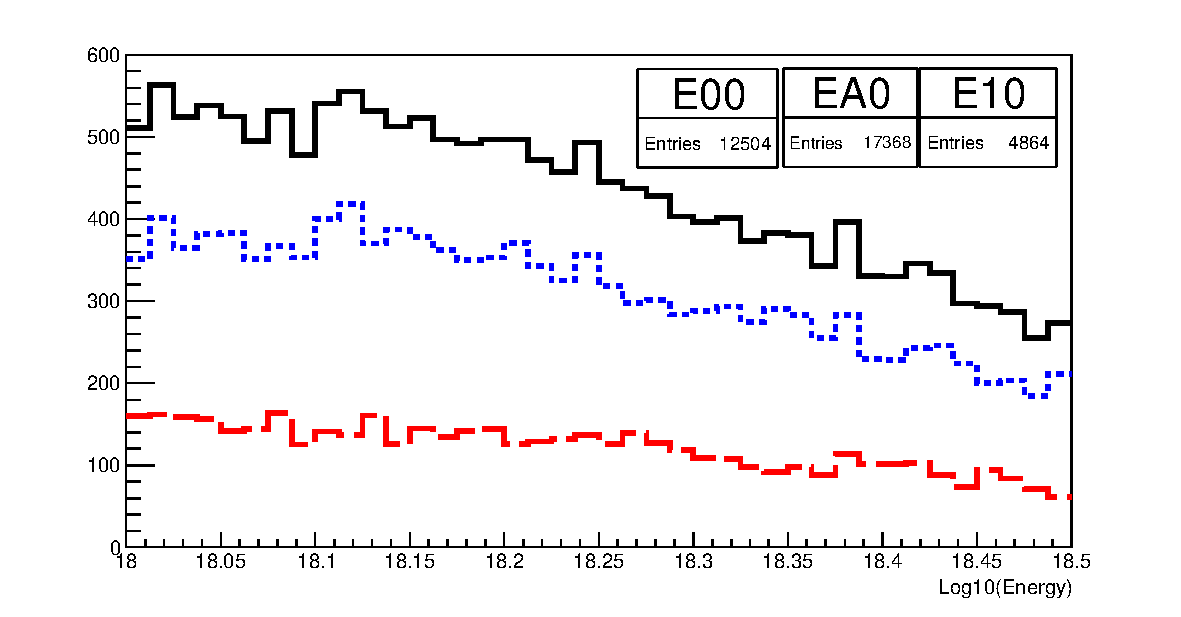
\includegraphics[width=\textwidth]{/home/tsudholz/PhD/Thesis/chapters/graphs/CloudFlags/EnergyHist_logE_18_0to18_5_Comb.pdf}
%\caption{Distribution of the energy of events within the bin of log(E) of 18.0 to 18.5. Black (EA0) denotes events that passed with cloud cut removed, blue (E00) denotes events that would pass the cloud cuts and red (E10) denotes events that would fail the cloud cuts. All other cuts used for the ICRC19 have been applied.}
%\end{figure}
%
%\begin{figure}
%\centering
%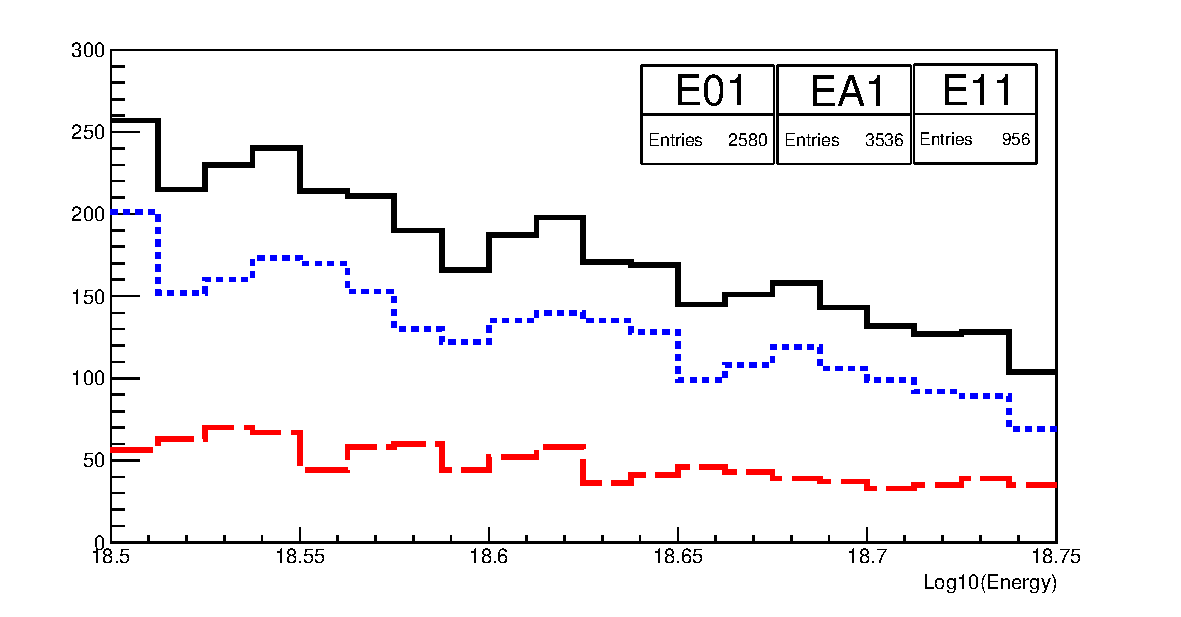
\includegraphics[width=\textwidth]{/home/tsudholz/PhD/Thesis/chapters/graphs/CloudFlags/EnergyHist_logE_18_5to18_75_Comb.pdf}
%\caption{Distribution of the energy of events within the bin of log(E) of 18.5 to 18.75. Black (EA1) denotes events that passed with cloud cut removed, blue (E01) denotes events that would pass the cloud cuts and red (E11) denotes events that would fail the cloud cuts. All other cuts used for the ICRC19 have been applied. }
%\end{figure}
%
%\begin{figure}
%\centering
%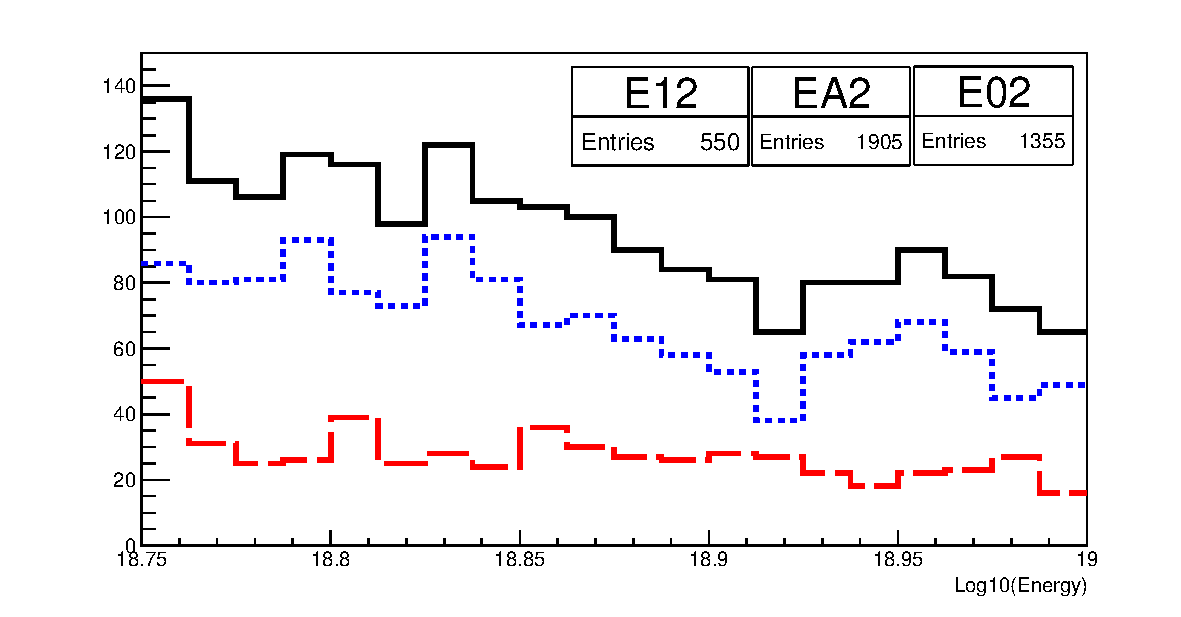
\includegraphics[width=\textwidth]{/home/tsudholz/PhD/Thesis/chapters/graphs/CloudFlags/EnergyHist_logE_18_75to19_0_Comb.pdf}
%\caption{Distribution of the energy of events within the bin of log(E) of 18.75 to 19.0. Black (EA2) denotes events that passed with cloud cut removed, blue (E12) denotes events that would pass the cloud cuts and red (E02) denotes events that would fail the cloud cuts. All other cuts used for the ICRC19 have been applied.}
%\end{figure}
%
%\begin{figure}
%\centering
%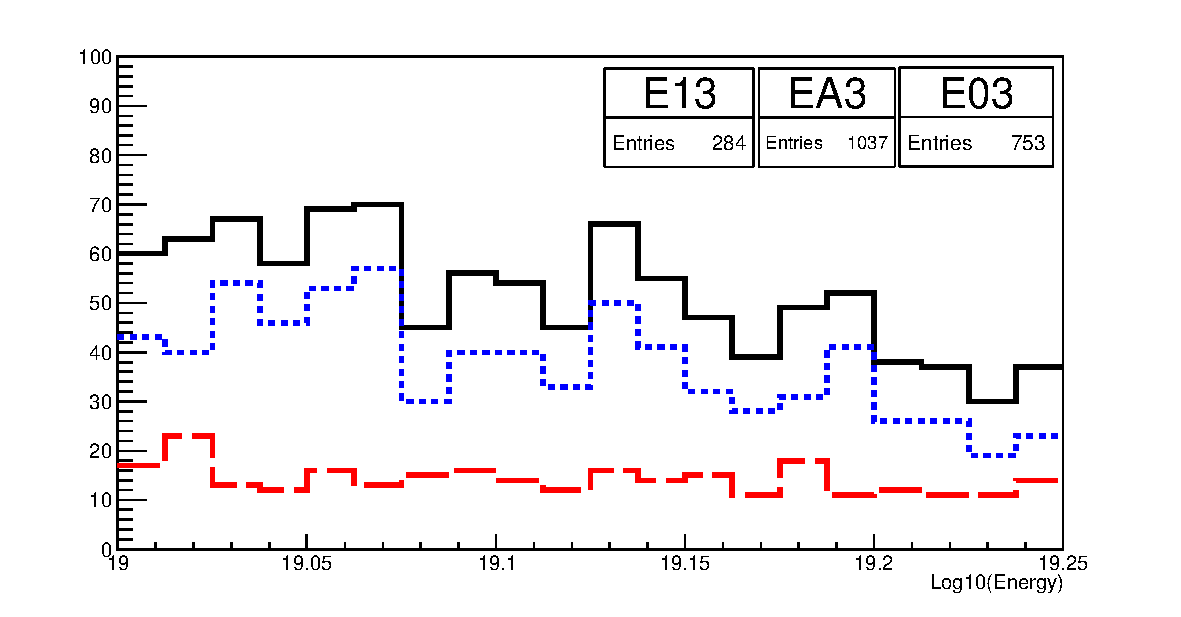
\includegraphics[width=\textwidth]{/home/tsudholz/PhD/Thesis/chapters/graphs/CloudFlags/EnergyHist_logE_19_0to19_25_Comb.pdf}
%\caption{Distribution of the energy of events within the bin of log(E) of 19.0 to 19.25. Black (EA3) denotes events that passed with cloud cut removed, blue (E13) denotes events that would pass the cloud cuts and red (E03) denotes events that would fail the cloud cuts. All other cuts used for the ICRC19 have been applied.}
%\end{figure}
%
%\begin{figure}
%\centering
%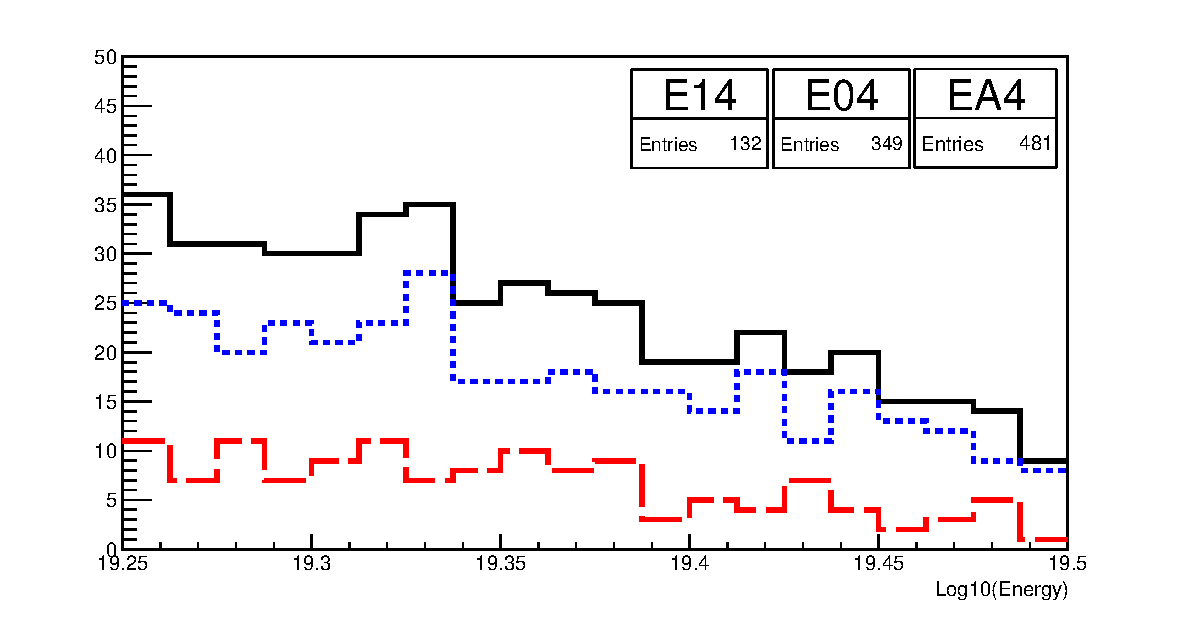
\includegraphics[width=\textwidth]{/home/tsudholz/PhD/Thesis/chapters/graphs/CloudFlags/EnergyHist_logE_19_25to19_5_Comb.pdf}
%\caption{Distribution of the energy of events within the bin of log(E) of 19.25 to 19.5. Black (EA4) denotes events that passed with cloud cut removed, blue (E14) denotes events that would pass the cloud cuts and red (E04) denotes events that would fail the cloud cuts. All other cuts used for the ICRC19 have been applied.}
%\end{figure}
%
%\begin{figure}
%\centering
%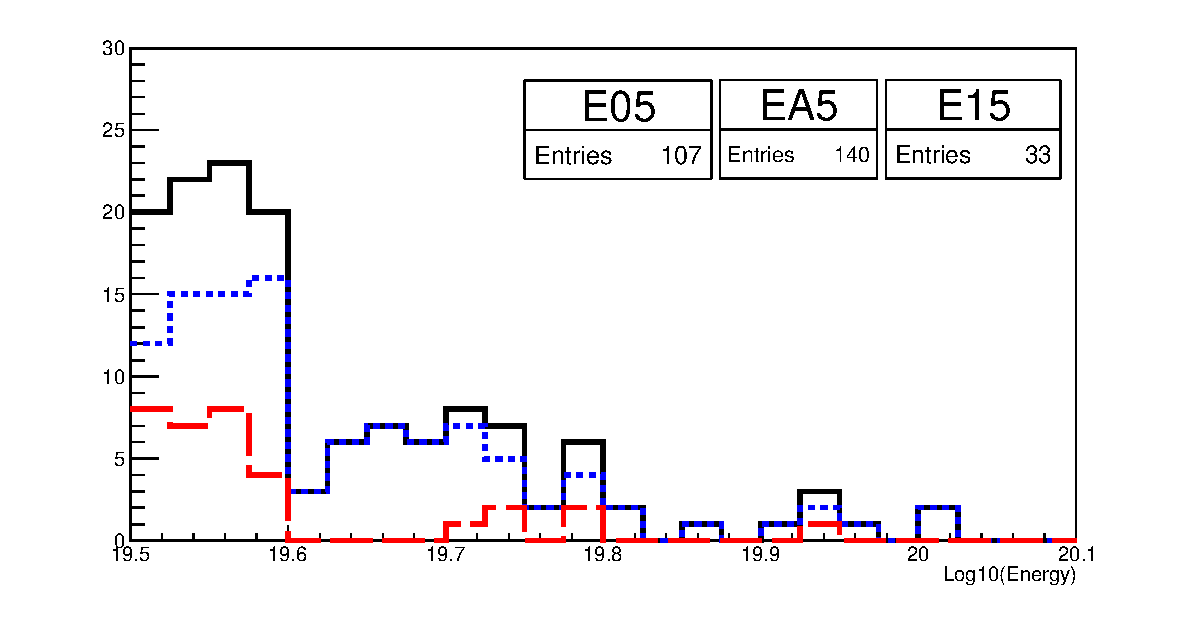
\includegraphics[width=\textwidth]{/home/tsudholz/PhD/Thesis/chapters/graphs/CloudFlags/EnergyHist_logE_Greater19_5_Comb.pdf}
%\caption{Distribution of the energy of events within the bin of log(E) of greater than 19.5. Black (EA5) denotes events that passed with cloud cut removed, blue (E15) denotes events that would pass the cloud cuts and red (E05) denotes events that would fail the cloud cuts. All other cuts used for the ICRC19 have been applied.}
%\end{figure}

% Xmax Distribution for Passed, Combined, Failed

\subsection{Xmax Distribution}

Comparison of Xmax distributions between data sets with the cloud cut, without the cloud cut and a data set that just contains events that would fail the cloud cut.

\begin{figure}
\centering
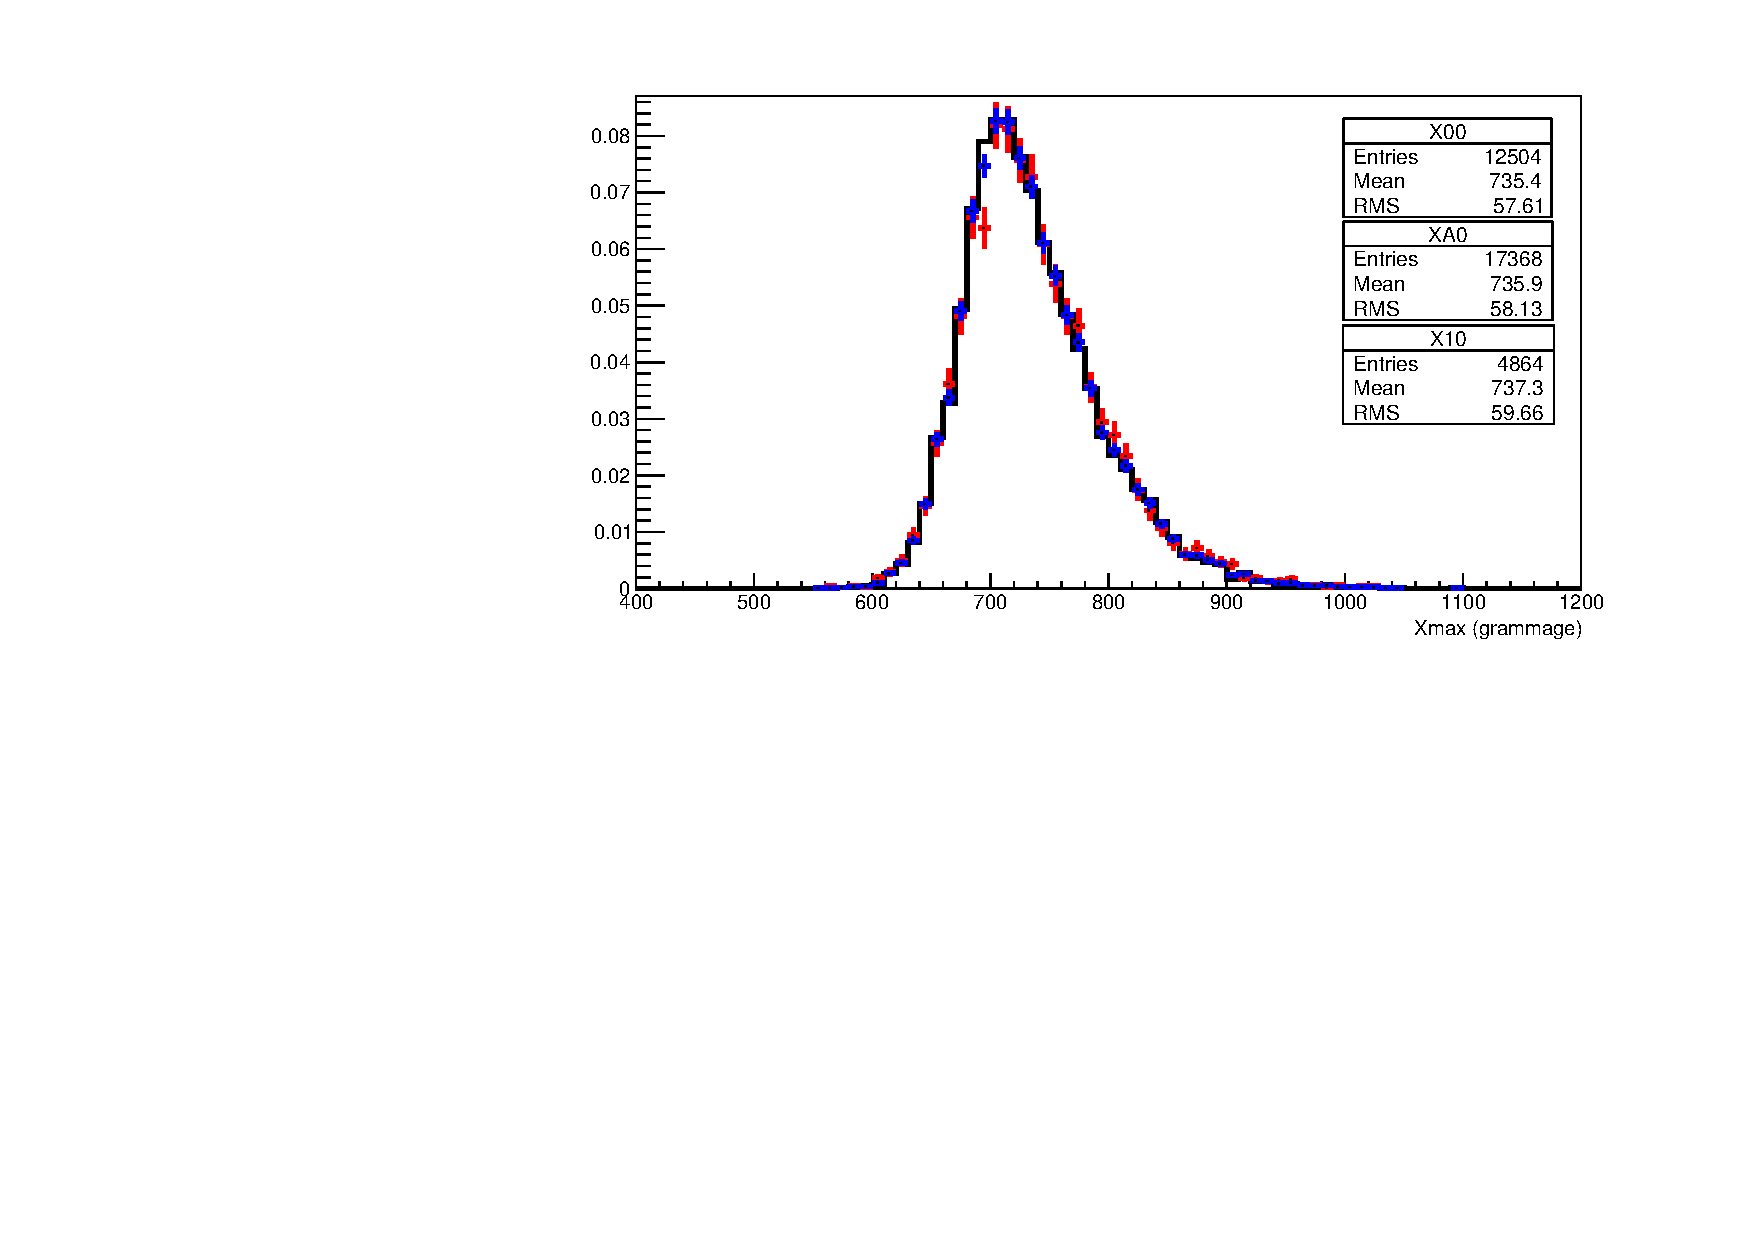
\includegraphics[width=\textwidth]{/home/tsudholz/PhD/Thesis/chapters/graphs/CloudFlags/NormHist_Xmax_logE_18_0to18_5_Comb.pdf}
\caption{Distribution of the Xmax of events within the bin of log(E) of 18.0 to 18.5. Black (XA0) denotes events that passed with cloud cut removed, blue (X00) denotes events that would pass the cloud cuts and red (X10) denotes events that would fail the cloud cuts. All other cuts used for the ICRC19 have been applied.}
\end{figure}

\begin{figure}
\centering
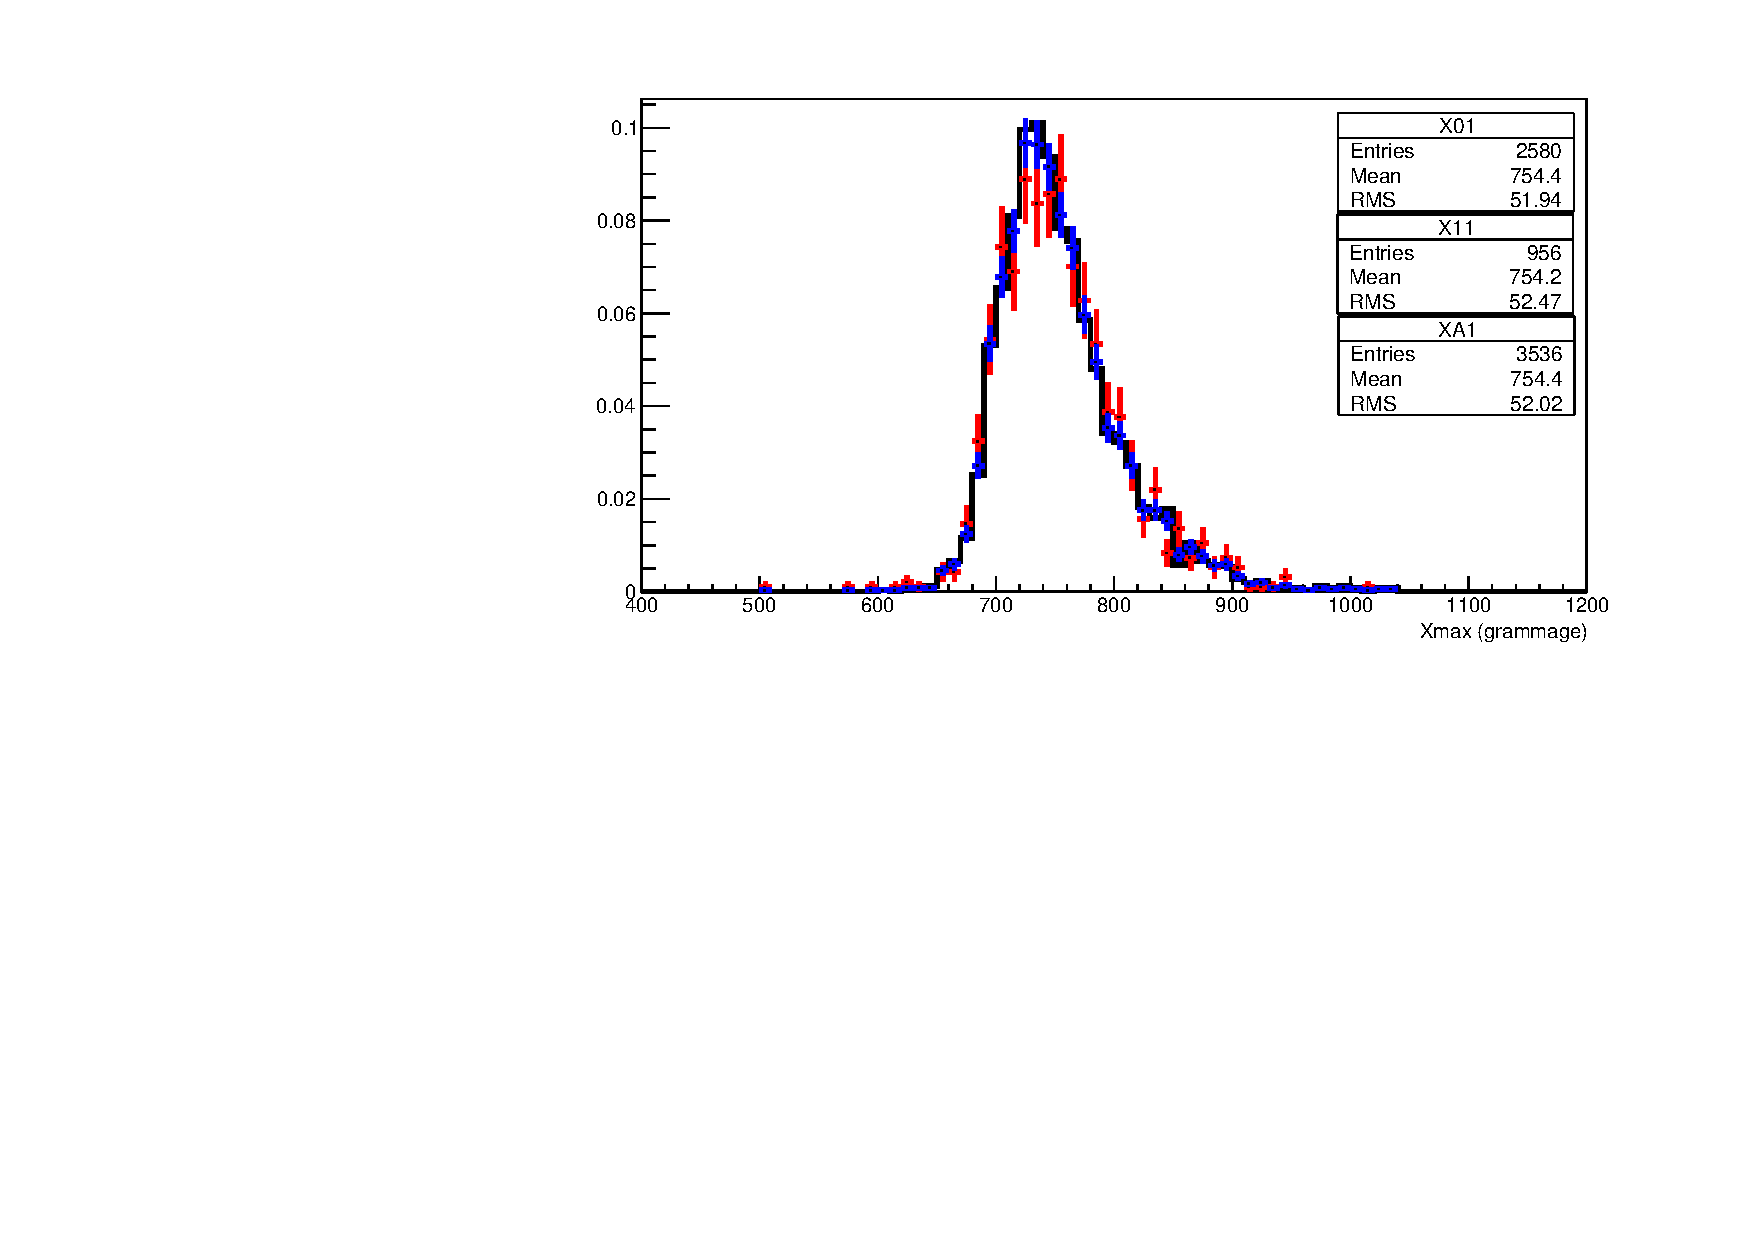
\includegraphics[width=\textwidth]{/home/tsudholz/PhD/Thesis/chapters/graphs/CloudFlags/NormHist_Xmax_logE_18_5to18_75_Comb.pdf}
\caption{Distribution of the Xmax of events within the bin of log(E) of 18.5 to 18.75. Black (XA1) denotes events that passed with cloud cut removed, blue (X01) denotes events that would pass the cloud cuts and red (X11) denotes events that would fail the cloud cuts. All other cuts used for the ICRC19 have been applied.}
\end{figure}

\begin{figure}
\centering
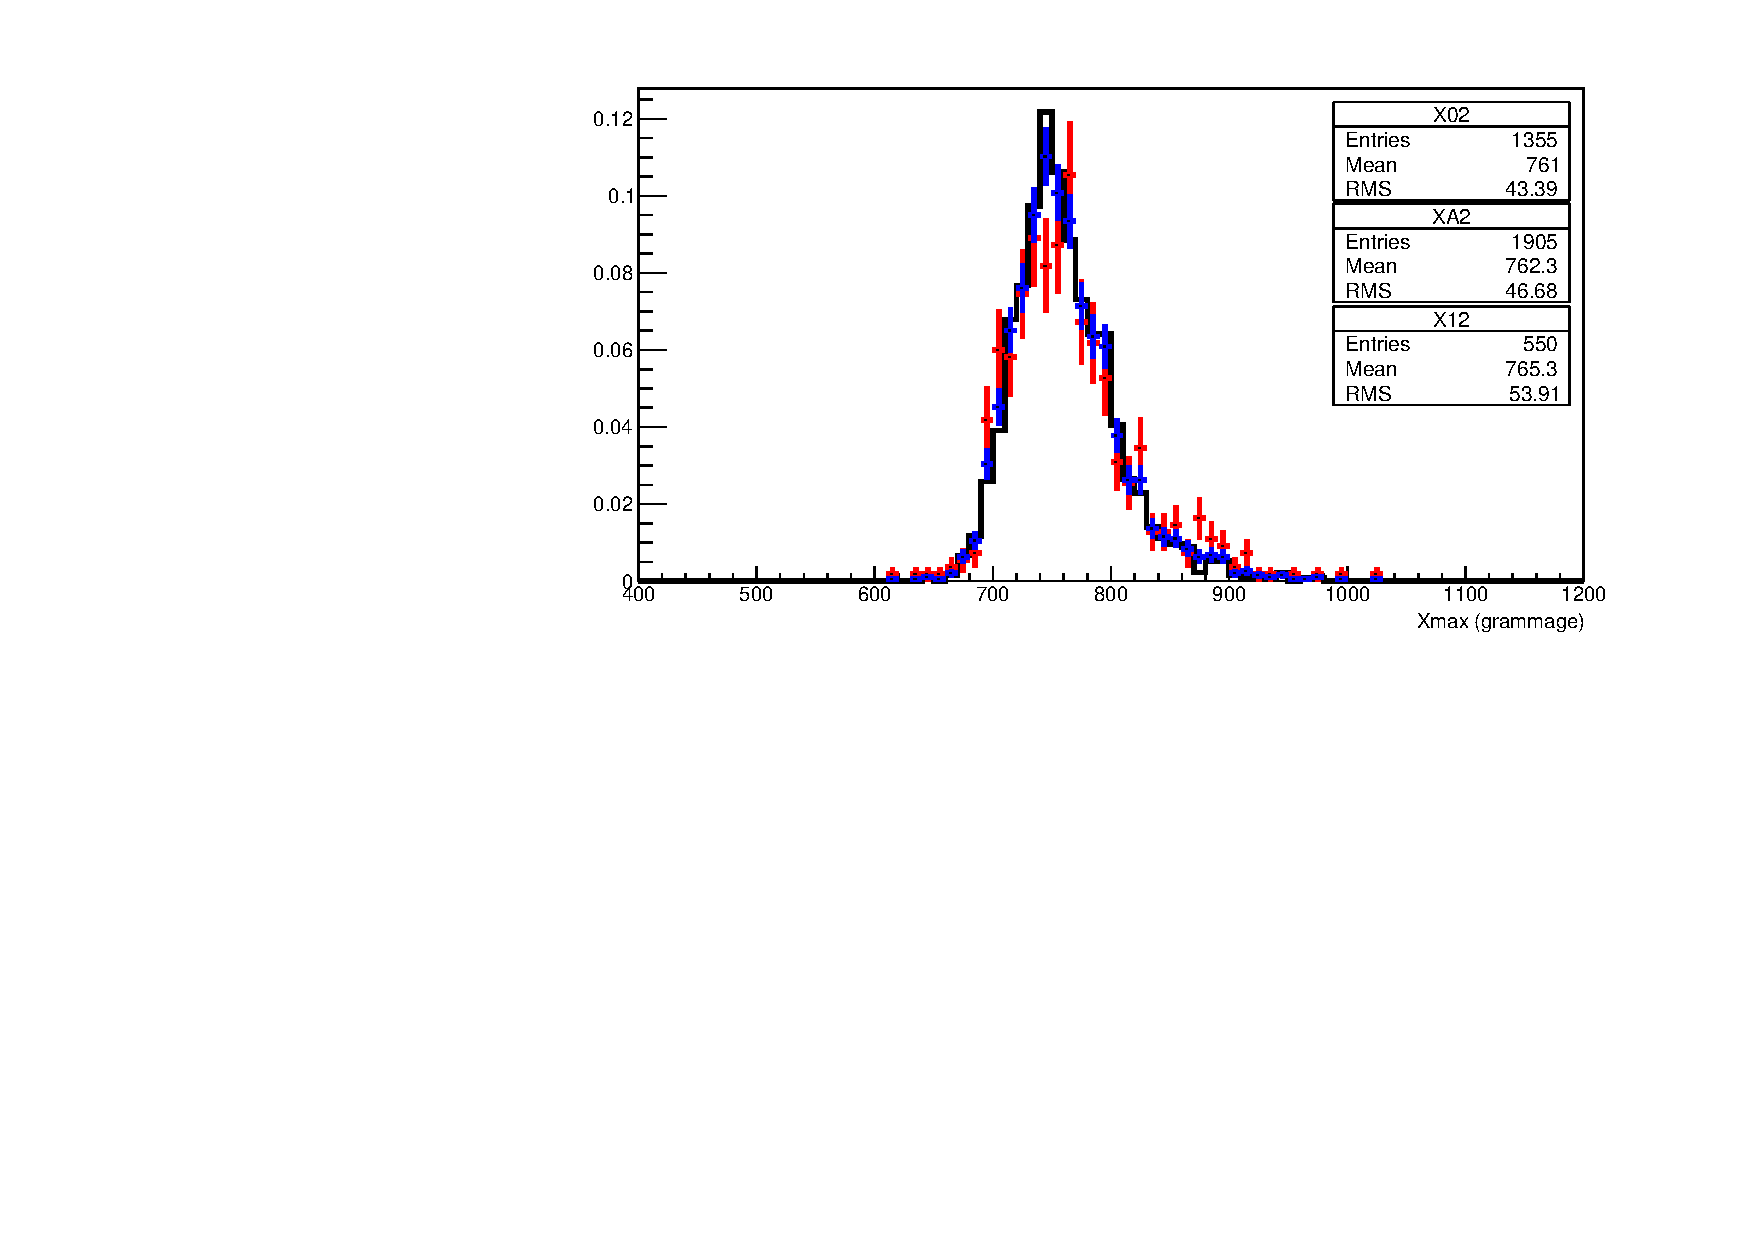
\includegraphics[width=\textwidth]{/home/tsudholz/PhD/Thesis/chapters/graphs/CloudFlags/NormHist_Xmax_logE_18_75to19_0_Comb.pdf}
\caption{Distribution of the Xmax of events within the bin of log(E) of 19.0 to 19.25. Black (XA2) denotes events that passed with cloud cut removed, blue (X02) denotes events that would pass the cloud cuts and red (X12) denotes events that would fail the cloud cuts. All other cuts used for the ICRC19 have been applied.}
\end{figure}

\begin{figure}
\centering
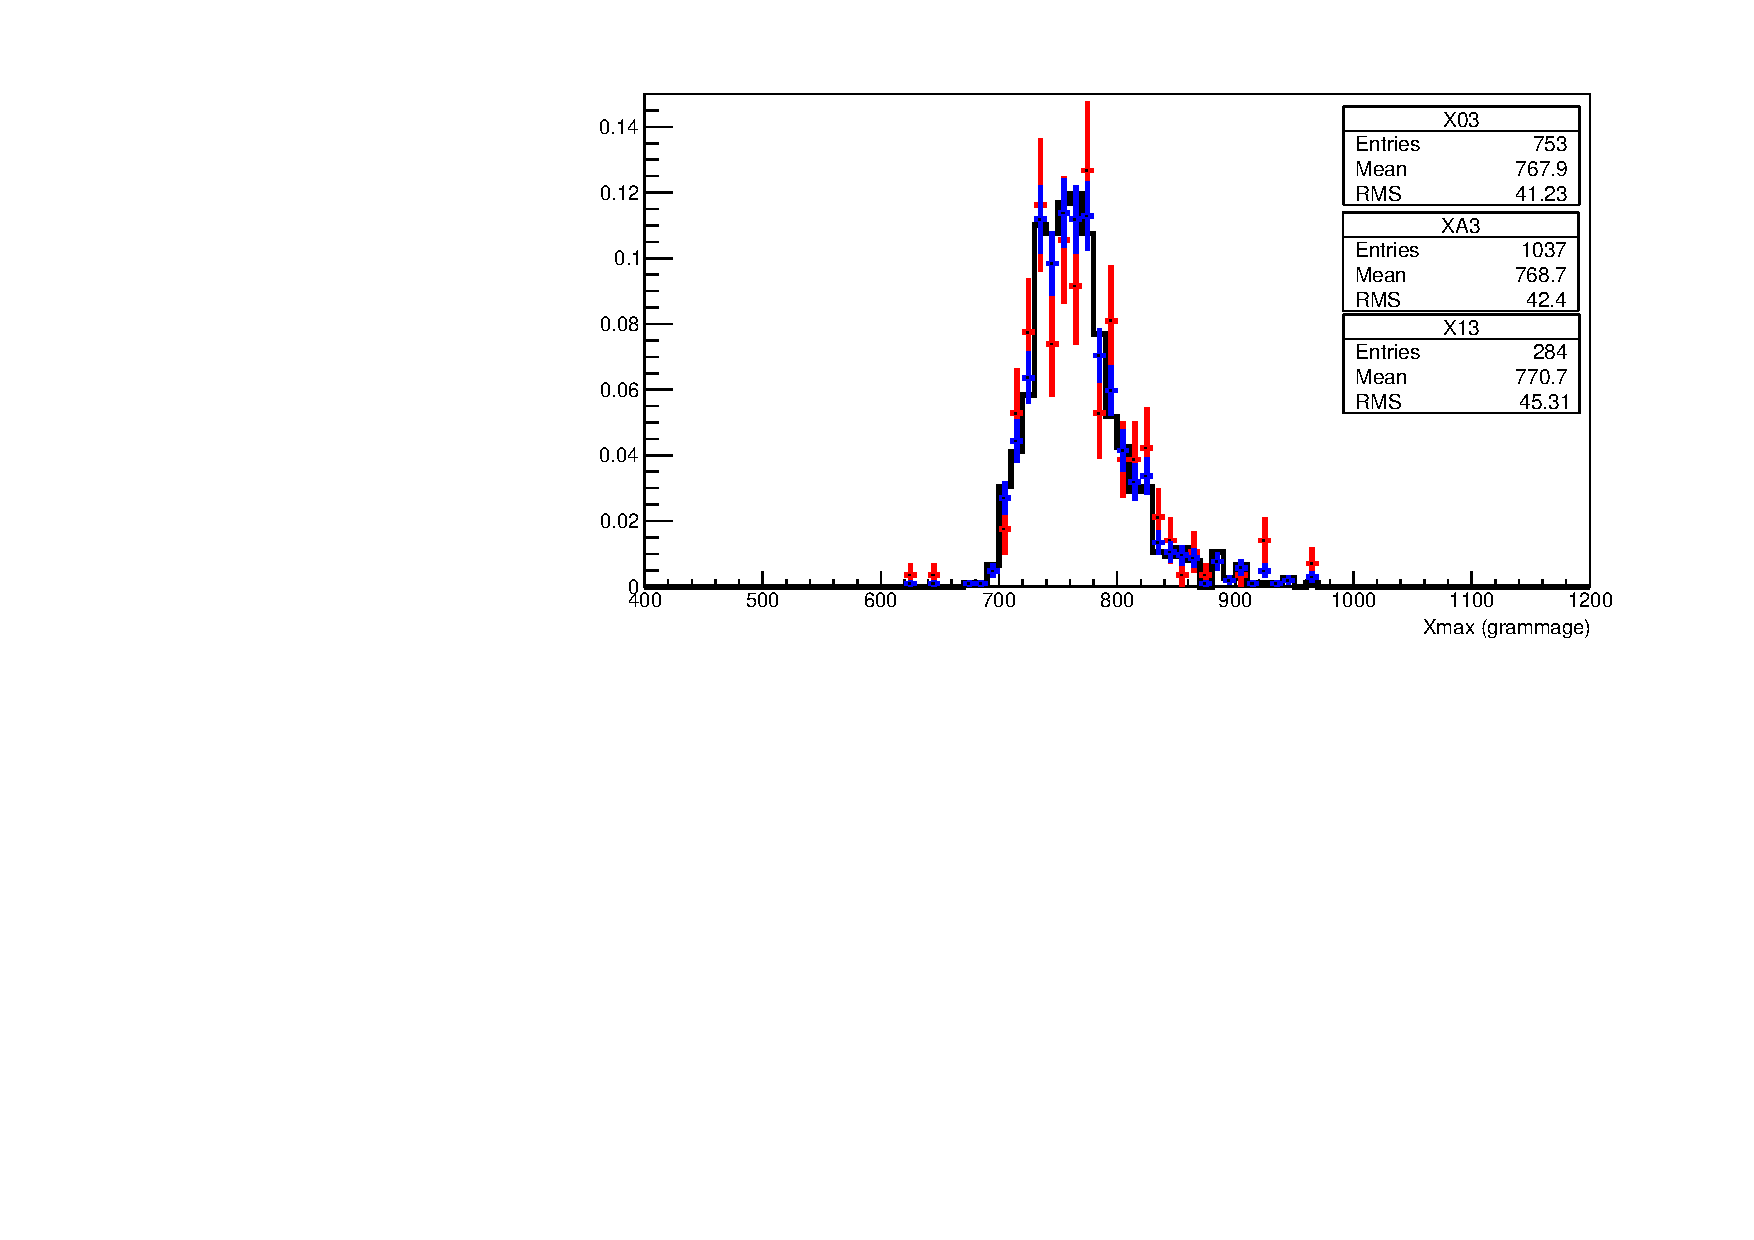
\includegraphics[width=\textwidth]{/home/tsudholz/PhD/Thesis/chapters/graphs/CloudFlags/NormHist_Xmax_logE_19_0to19_25_Comb.pdf}
\caption{Distribution of the Xmax of events within the bin of log(E) of 19.0 to 19.25. Black (XA3) denotes events that passed with cloud cut removed, blue (X03) denotes events that would pass the cloud cuts and red (X13) denotes events that would fail the cloud cuts. All other cuts used for the ICRC19 have been applied.}
\end{figure}

\begin{figure}
\centering
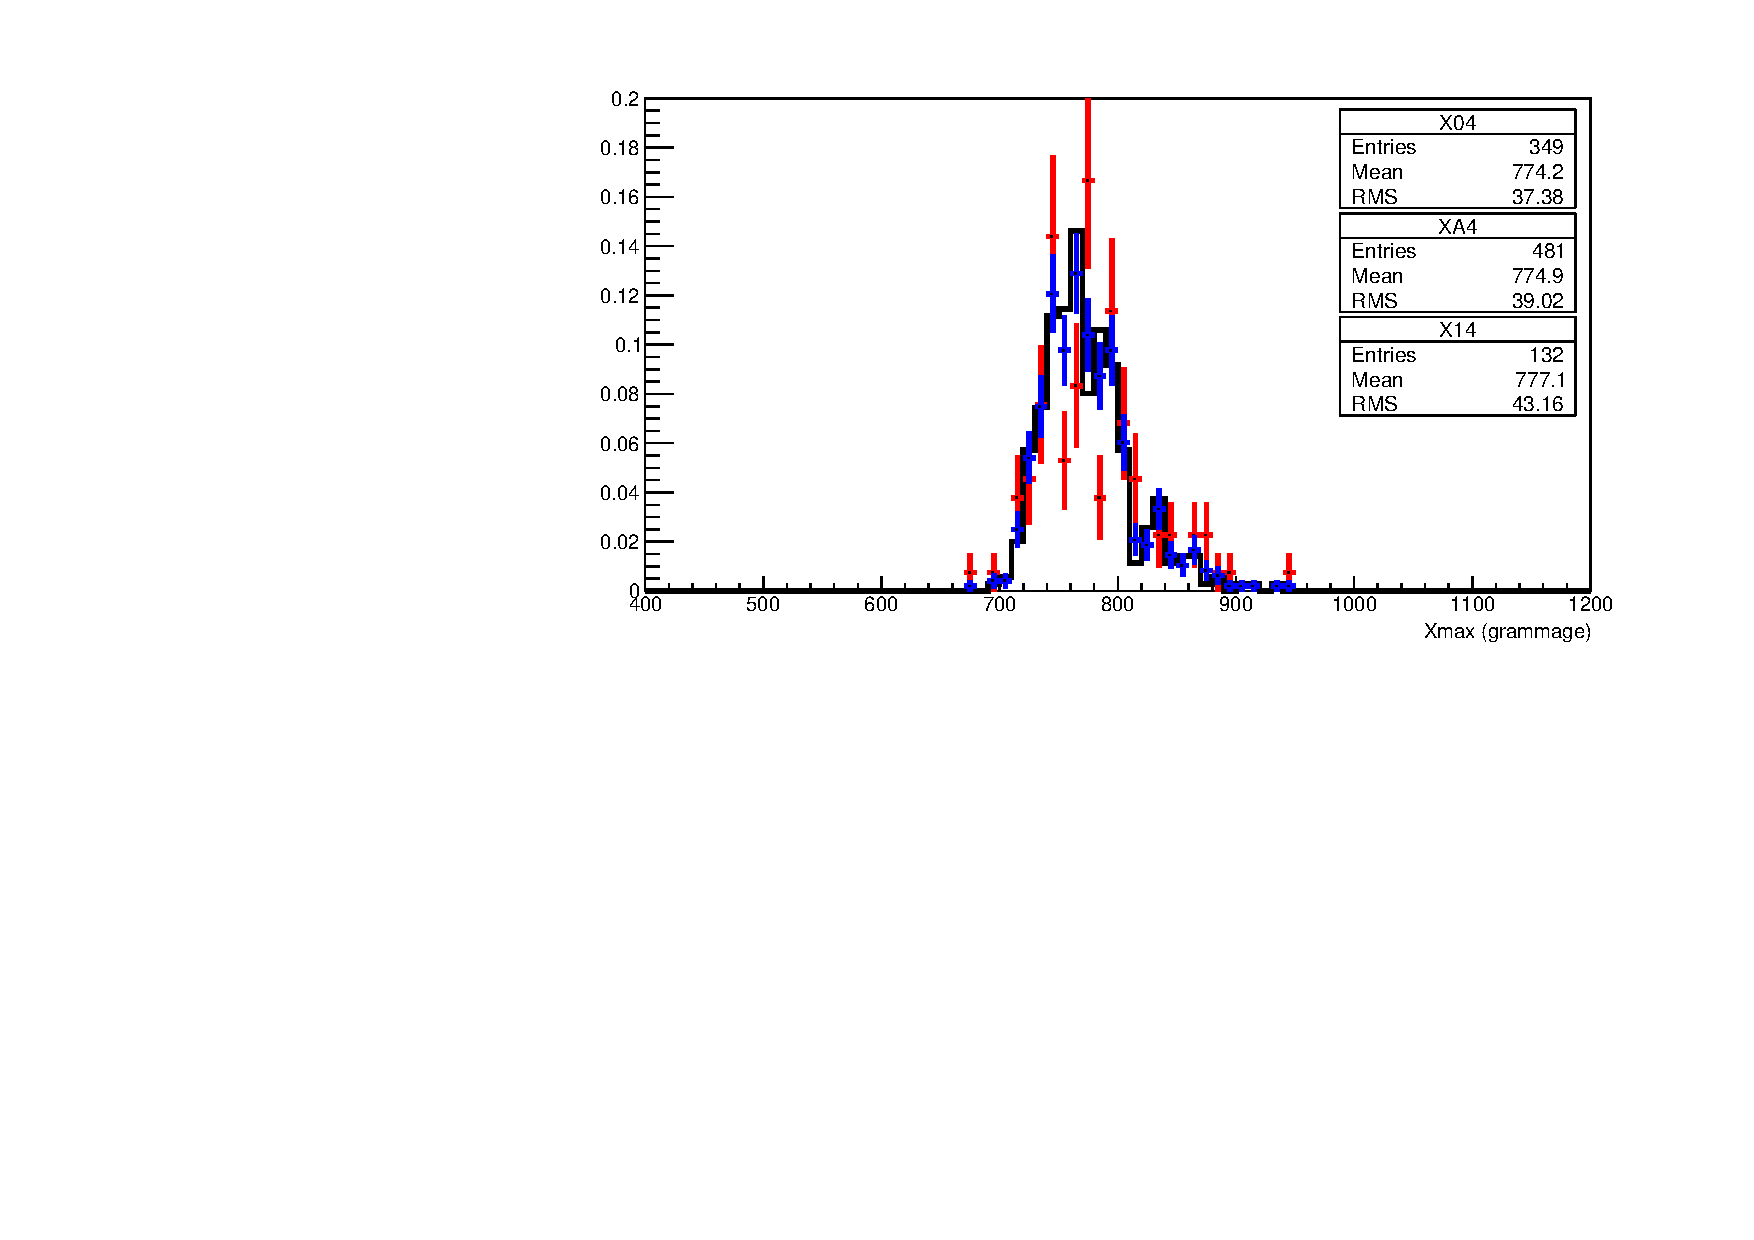
\includegraphics[width=\textwidth]{/home/tsudholz/PhD/Thesis/chapters/graphs/CloudFlags/NormHist_Xmax_logE_19_25to19_5_Comb.pdf}
\caption{Distribution of the Xmax of events within the bin of log(E) of 19.25 to 19.5. Black (XA4) denotes events that passed with cloud cut removed, blue (X04) denotes events that would pass the cloud cuts and red (X14) denotes events that would fail the cloud cuts. All other cuts used for the ICRC19 have been applied.}
\end{figure}

\begin{figure}
\centering
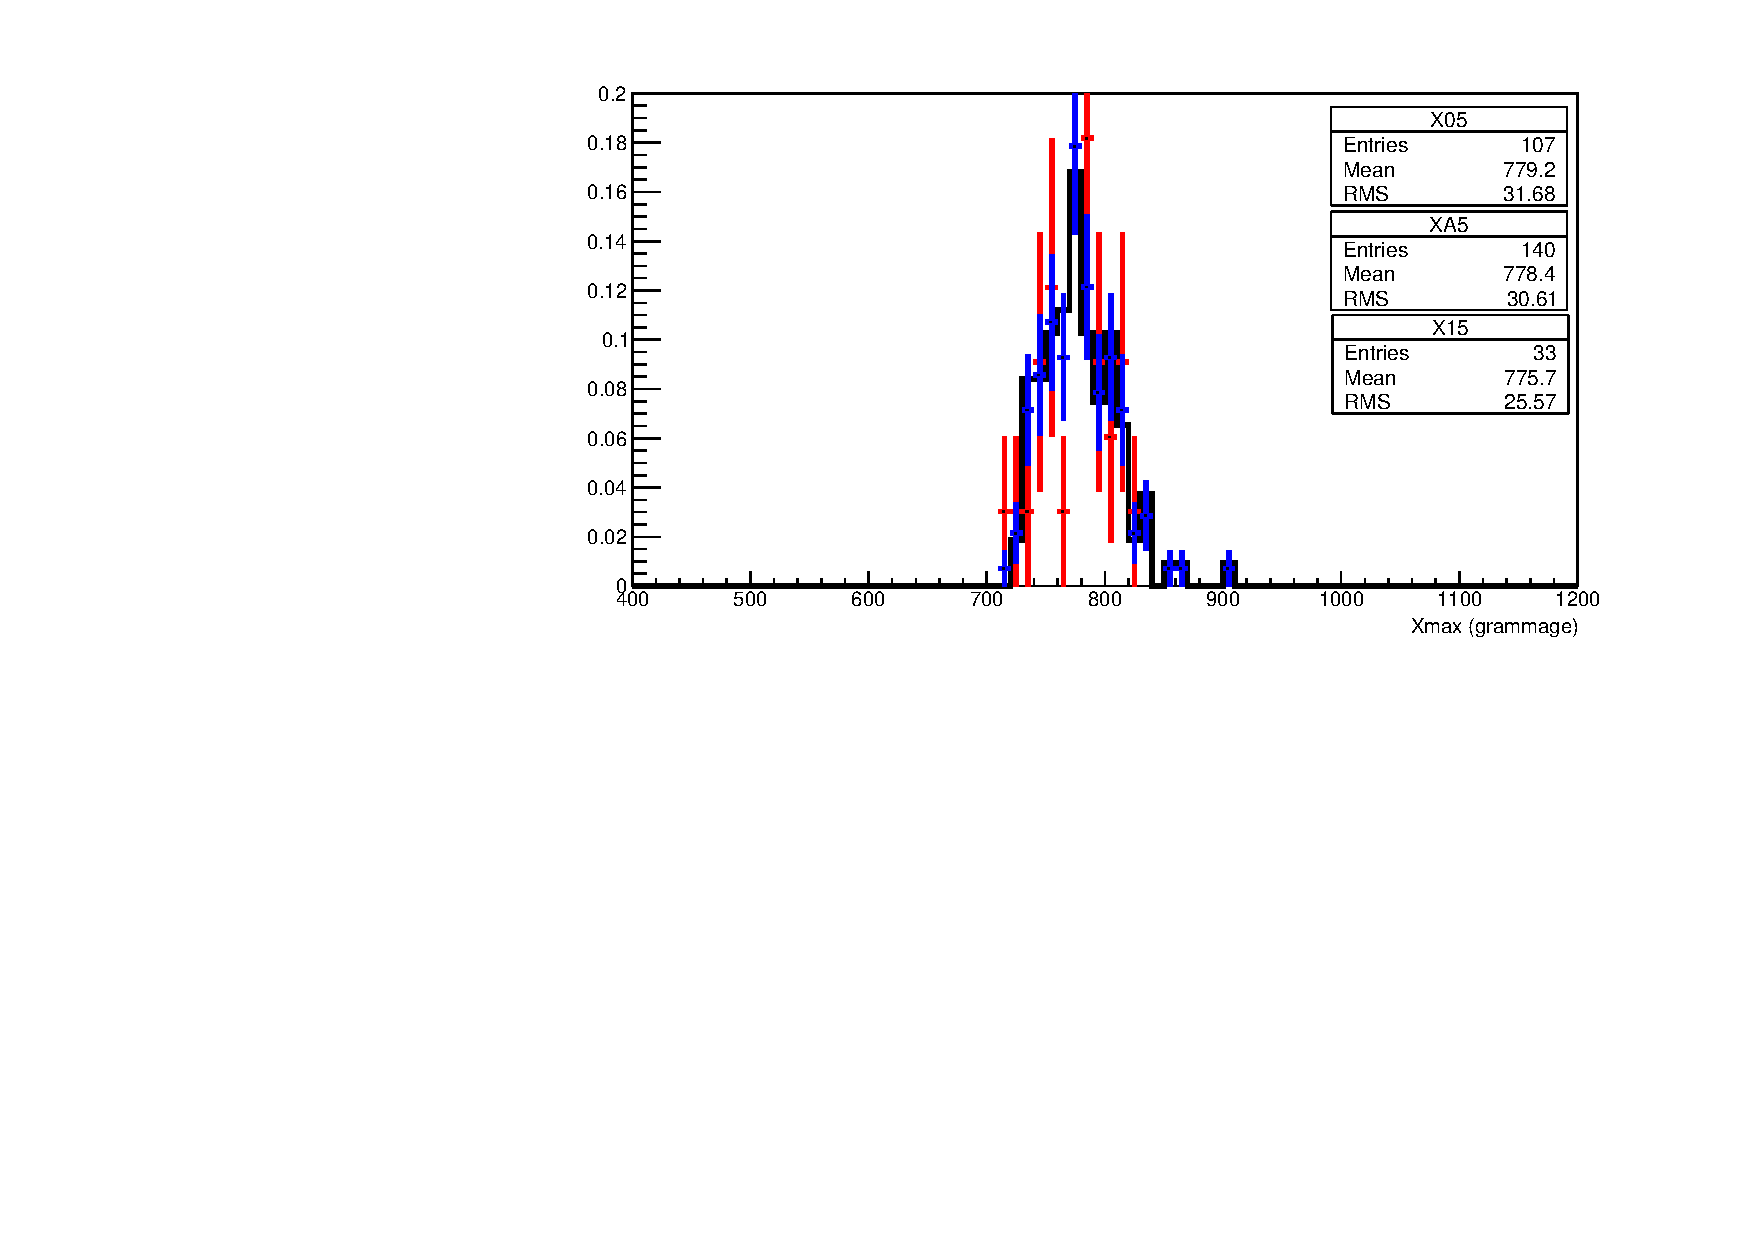
\includegraphics[width=\textwidth]{/home/tsudholz/PhD/Thesis/chapters/graphs/CloudFlags/NormHist_Xmax_logE_Greater19_5_Comb.pdf}
\caption{Distribution of the Xmax of events within the bin of log(E) of greater than 19.5. Black (XA5) denotes events that passed with cloud cut removed, blue (X05) denotes events that would pass the cloud cuts and red (X15) denotes events that would fail the cloud cuts. All other cuts used for the ICRC19 have been applied.}
\end{figure}

% Xmax Distribution for Failed only

\subsubsection{Xmax Distribution for Events that Failed Cloud Cut}

\begin{figure}
\centering
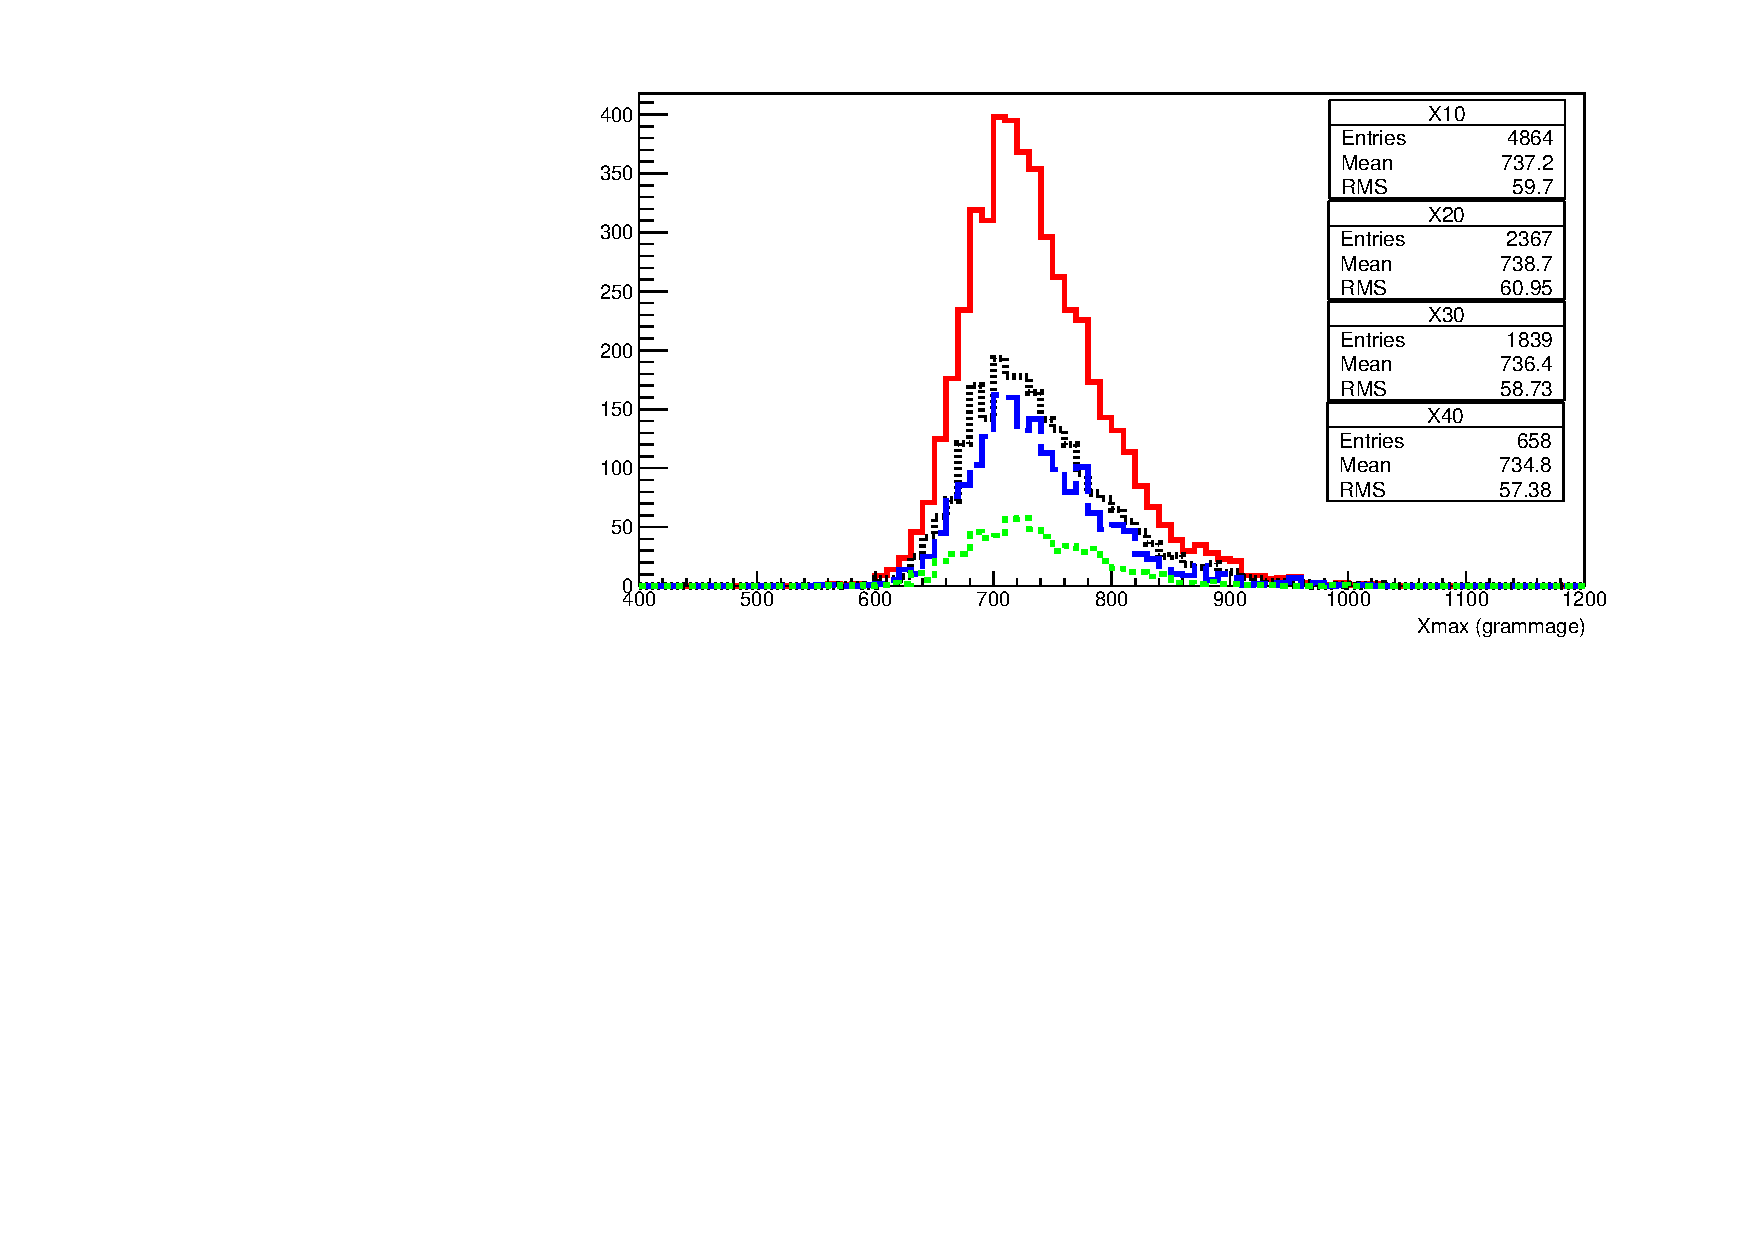
\includegraphics[width=\textwidth]{/home/tsudholz/PhD/Thesis/chapters/graphs/CloudFlags/NormHist_Xmax_FailedCloudCut_logE_18_0to18_5_Comb.pdf}
\caption{Distribution of the energy of events within the bin of log(E) of 18.0 to 18.5. Red (X10) denotes all event that failed the cloud cuts, black (X20) denotes events that failed the cloud camera/lidar cut, blue (X30) denotes events that failed the GOES data cut and green (X40) are events that have fail a combination of CLF/XLF, GOES and Cloud camera cut.}
\end{figure}

\begin{figure}
\centering
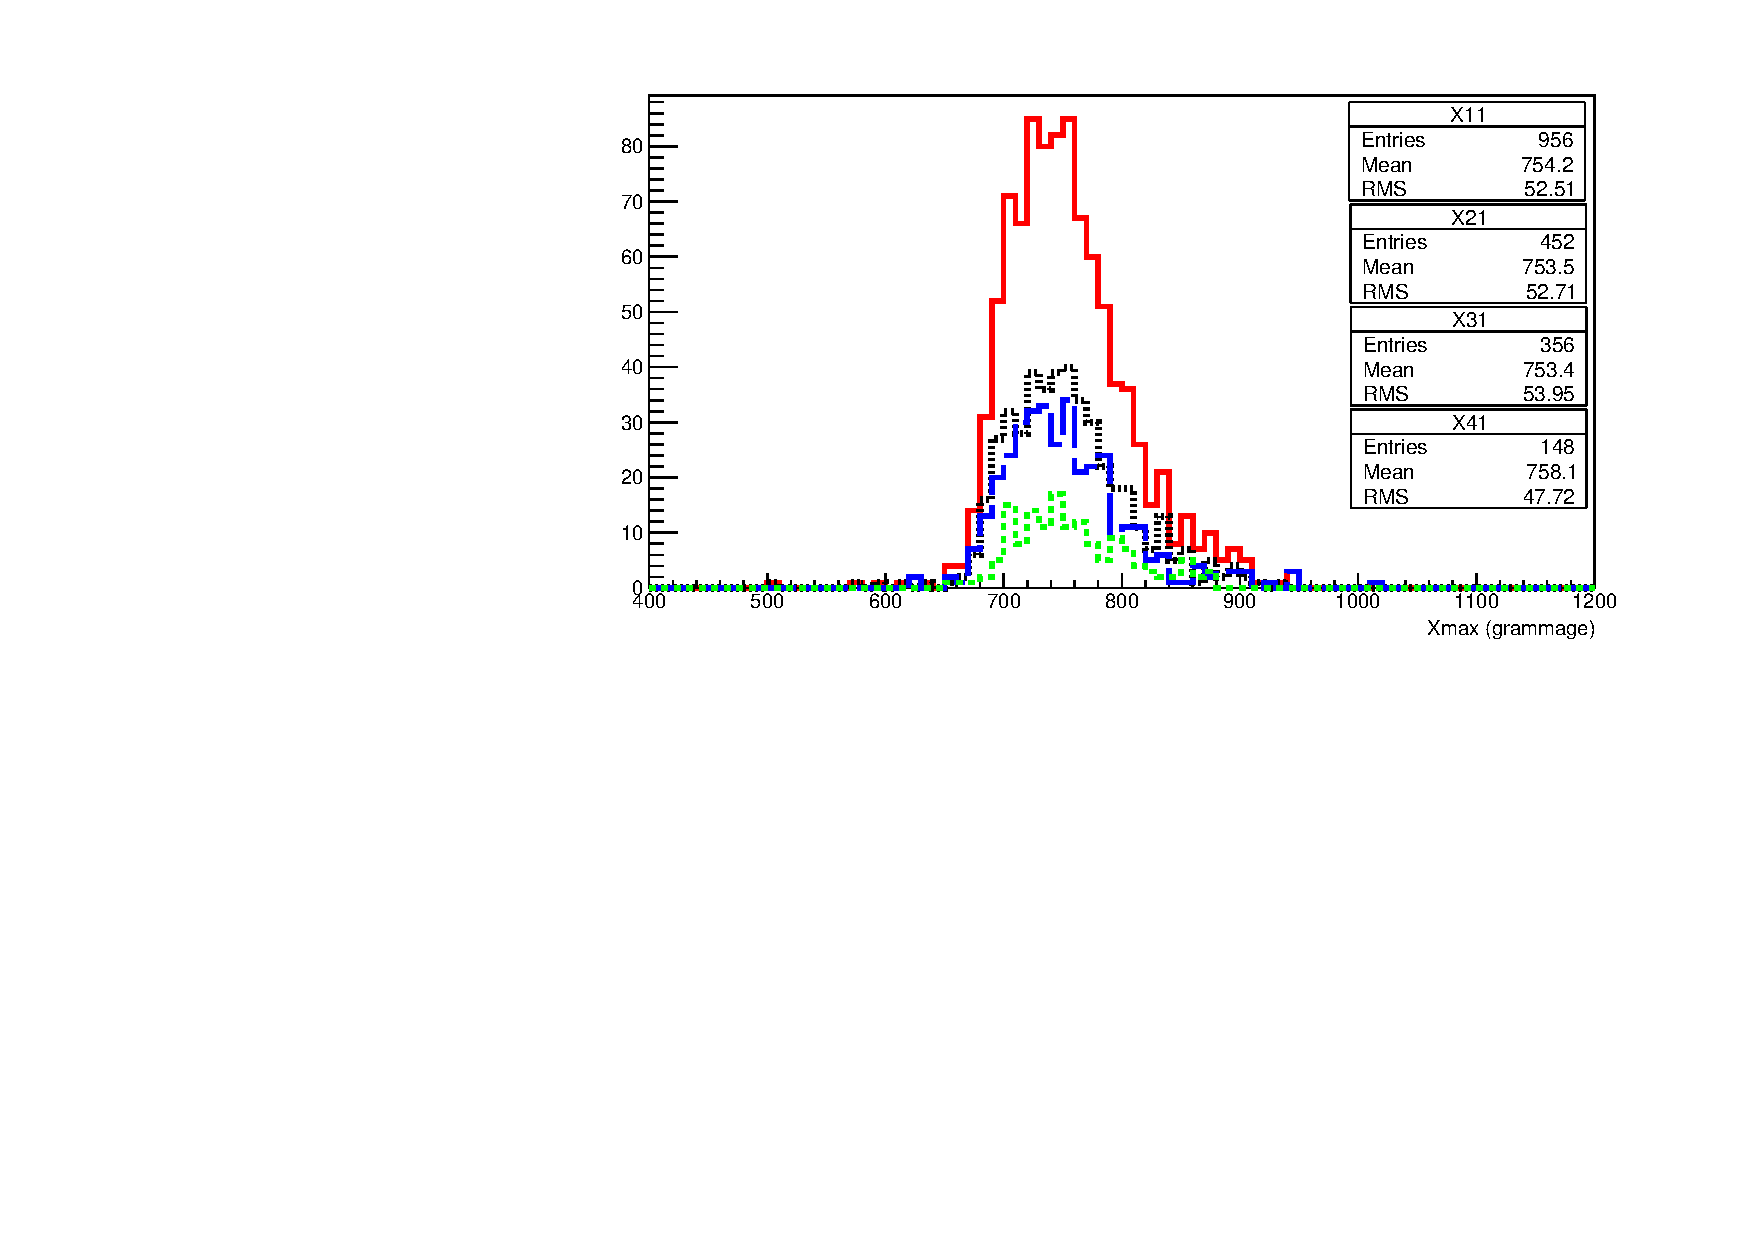
\includegraphics[width=\textwidth]{/home/tsudholz/PhD/Thesis/chapters/graphs/CloudFlags/NormHist_Xmax_FailedCloudCut_logE_18_5to18_75_Comb.pdf}
\caption{Distribution of the energy of events within the bin of log(E) of 18.5 to 18.75. Red (X11) denotes all event that failed the cloud cuts, black (X21) denotes events that failed the cloud camera/lidar cut, blue (X31) denotes events that failed the GOES data cut and green (X41) are events that have fail a combination of CLF/XLF, GOES and Cloud camera cut.}
\end{figure}

\begin{figure}
\centering
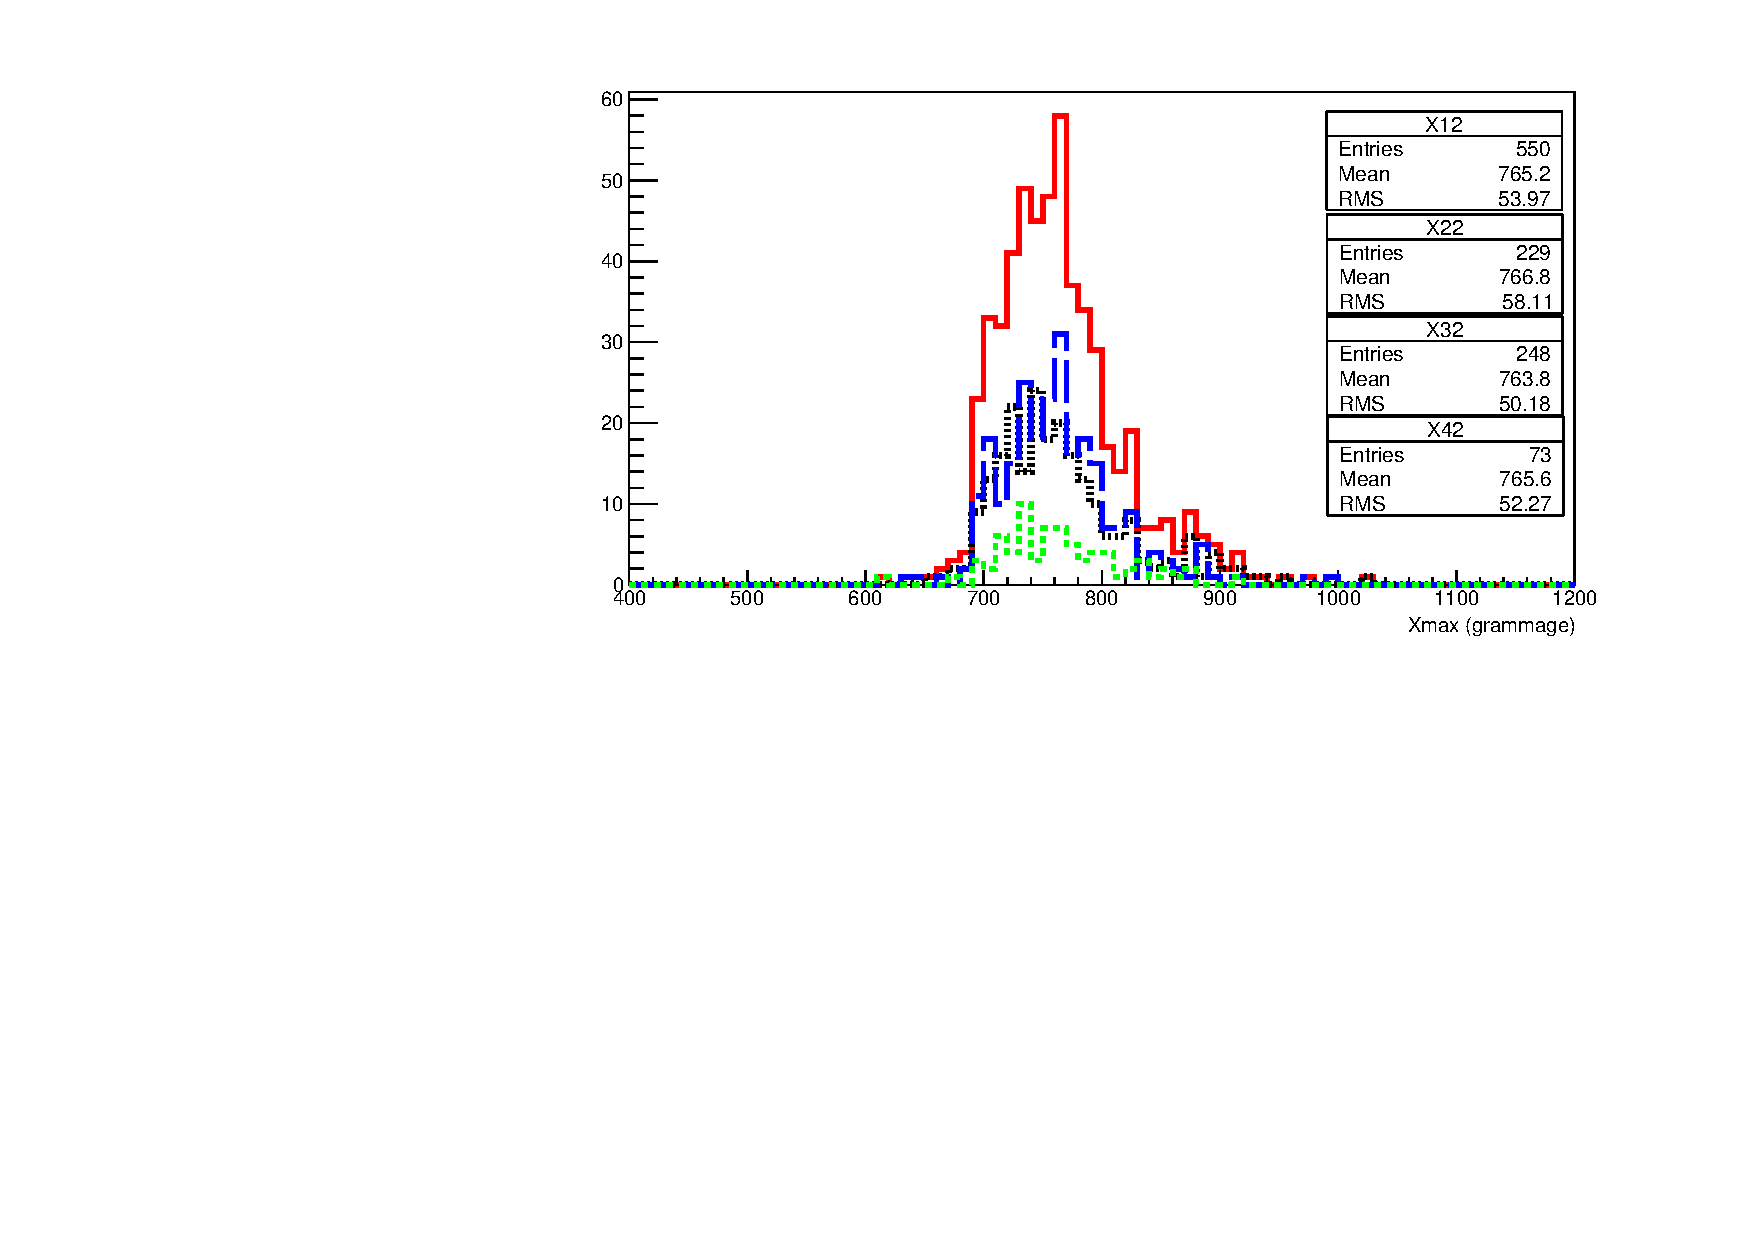
\includegraphics[width=\textwidth]{/home/tsudholz/PhD/Thesis/chapters/graphs/CloudFlags/NormHist_Xmax_FailedCloudCut_logE_18_75to19_0_Comb.pdf}
\caption{Distribution of the energy of events within the bin of log(E) of 18.75 to 19.0. Red (X12) denotes all event that failed the cloud cuts, black (X22) denotes events that failed the cloud camera/lidar cut, blue (X32) denotes events that failed the GOES data cut and green (X42) are events that have fail a combination of CLF/XLF, GOES and Cloud camera cut.}
\end{figure}

\begin{figure}
\centering
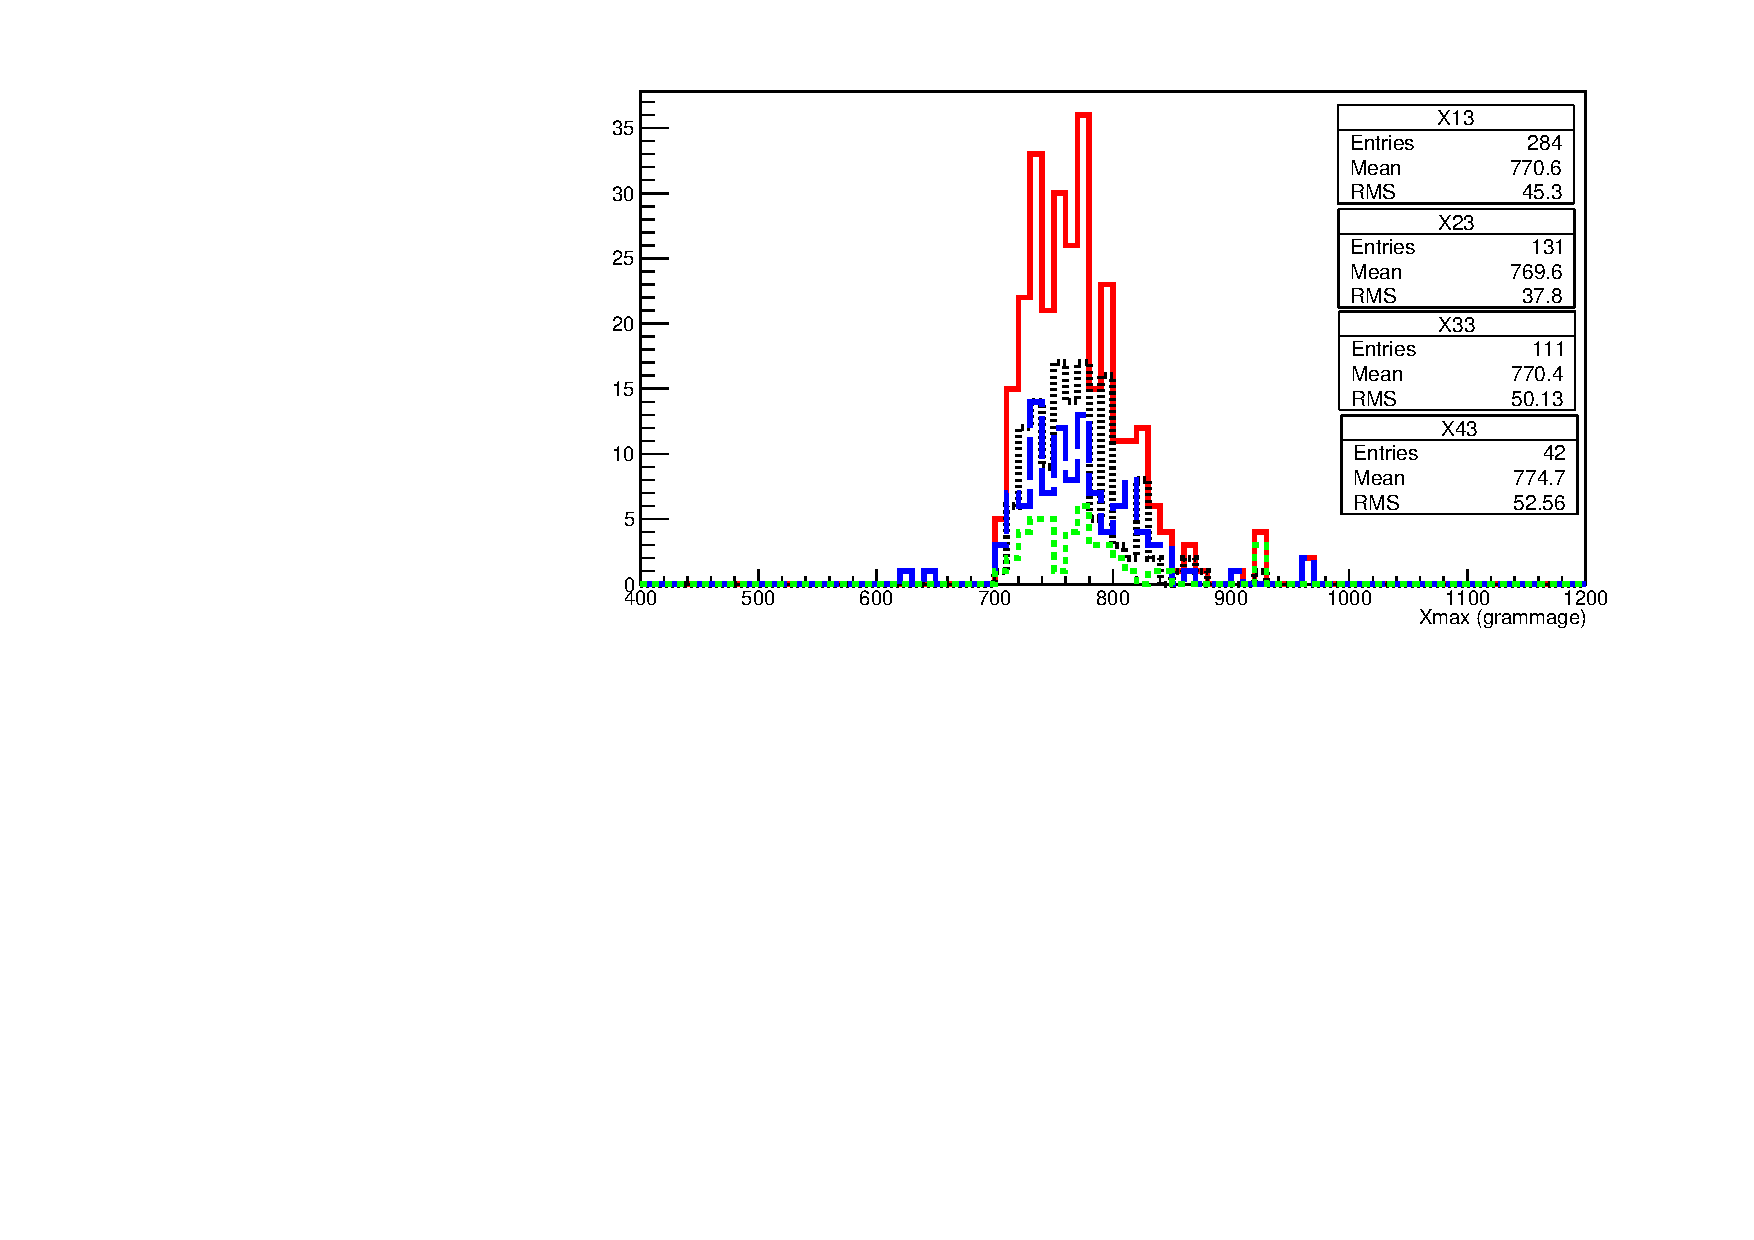
\includegraphics[width=\textwidth]{/home/tsudholz/PhD/Thesis/chapters/graphs/CloudFlags/NormHist_Xmax_FailedCloudCut_logE_19_0to19_25_Comb.pdf}
\caption{Distribution of the energy of events within the bin of log(E) of 19.0 to 19.25. Red (X13) denotes all event that failed the cloud cuts, black (X23) denotes events that failed the cloud camera/lidar cut, blue (X33) denotes events that failed the GOES data cut and green (X43) are events that have fail a combination of CLF/XLF, GOES and Cloud camera cut.}
\end{figure}

\begin{figure}
\centering
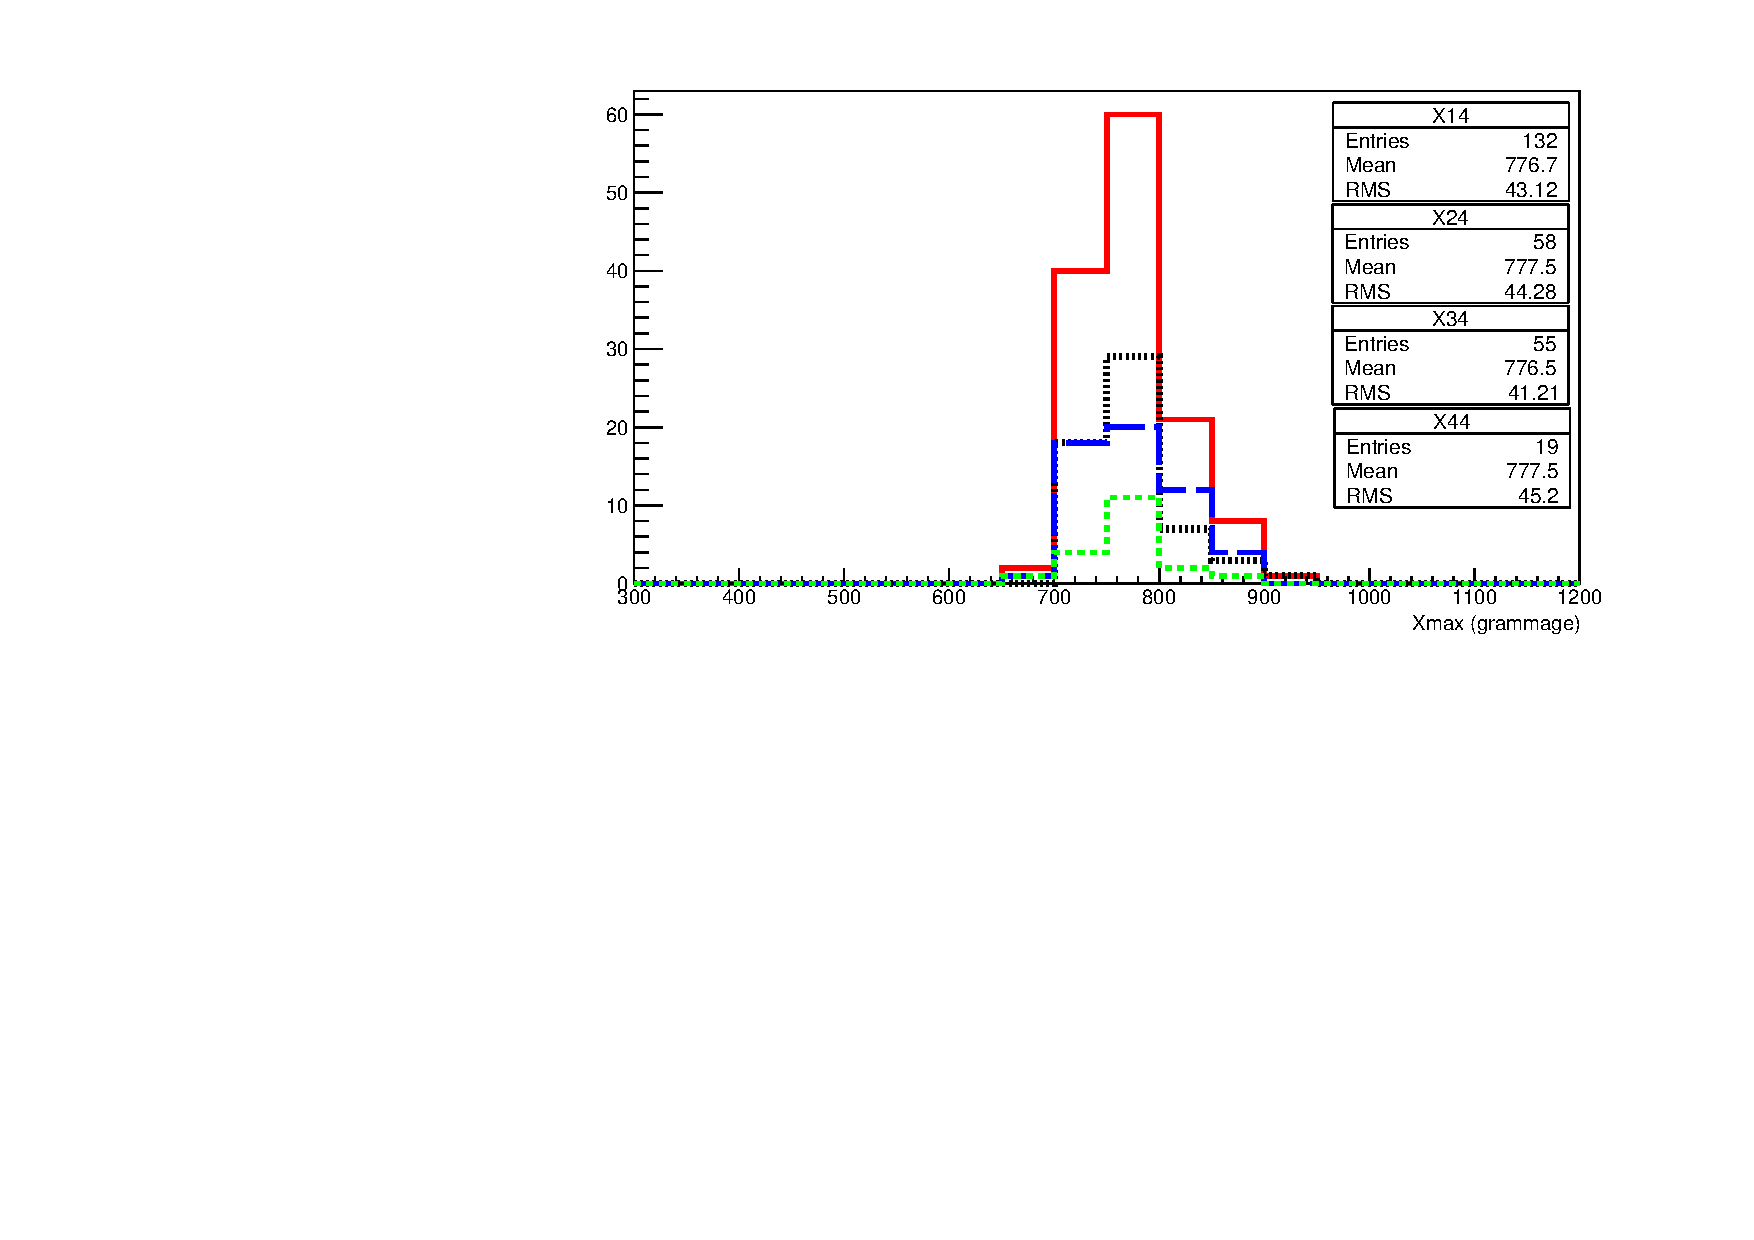
\includegraphics[width=\textwidth]{/home/tsudholz/PhD/Thesis/chapters/graphs/CloudFlags/NormHist_Xmax_FailedCloudCut_logE_19_25to19_5_Comb.pdf}
\caption{Distribution of the energy of events within the bin of log(E) of 19.25 to 19.5. Red (X14) denotes all event that failed the cloud cuts, black (X24) denotes events that failed the cloud camera/lidar cut, blue (X34) denotes events that failed the GOES data cut and green (X44) are events that have fail a combination of CLF/XLF, GOES and Cloud camera cut.}
\end{figure}

\begin{figure}
\centering
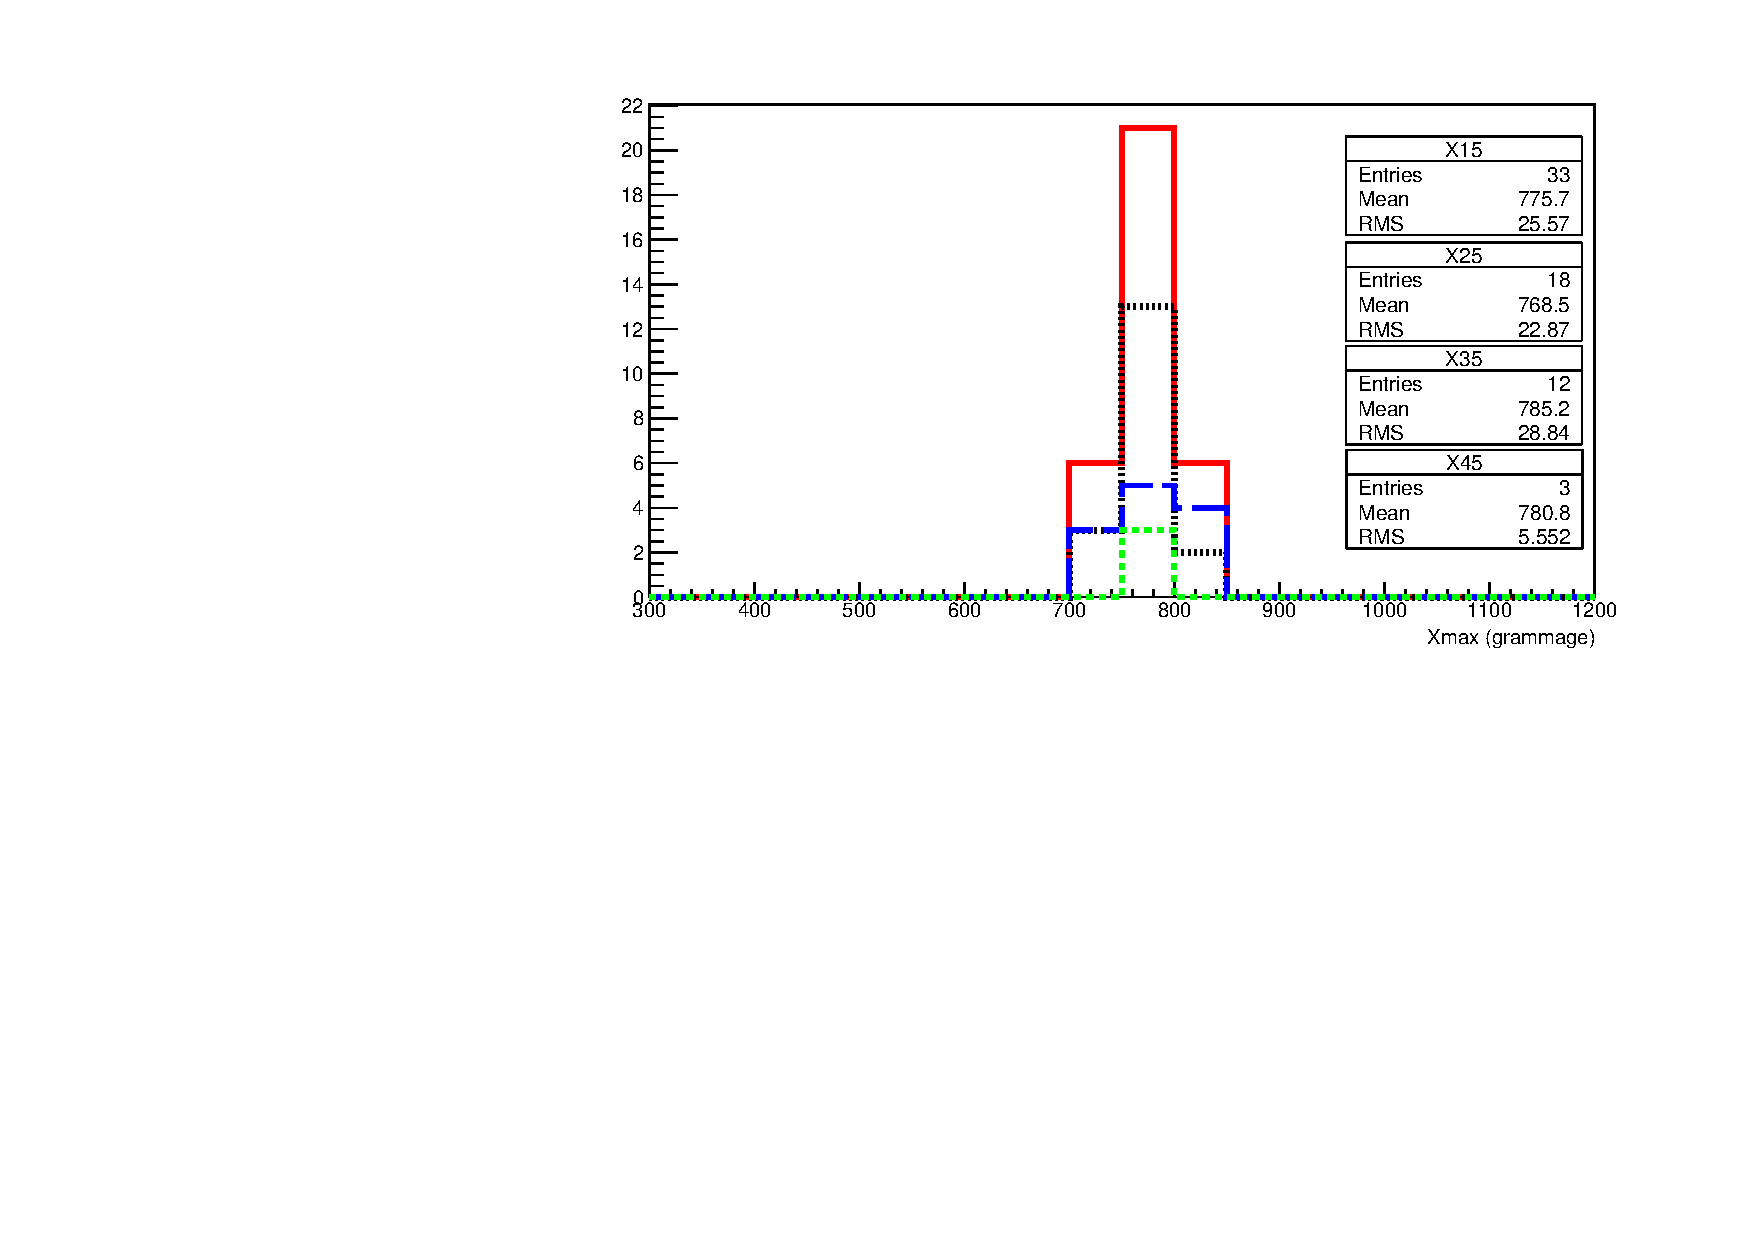
\includegraphics[width=\textwidth]{/home/tsudholz/PhD/Thesis/chapters/graphs/CloudFlags/NormHist_Xmax_FailedCloudCut_logE_Greater19_5_Comb.pdf}
\caption{Distribution of the energy of events within the bin of log(E) of greater than 19.5. Red (X15) denotes all event that failed the cloud cuts, black (X25) denotes events that failed the cloud camera/lidar cut, blue (X35) denotes events that failed the GOES data cut and green (X45) are events that have fail a combination of CLF/XLF, GOES and Cloud camera cut.}
\end{figure}

\subsection{Examples of Events that have failed Cloud Selection Cuts from EventBrowser}

% Events that would fail the cloud cut only

\begin{figure}
\centering
  \settoheight{\tempheight}{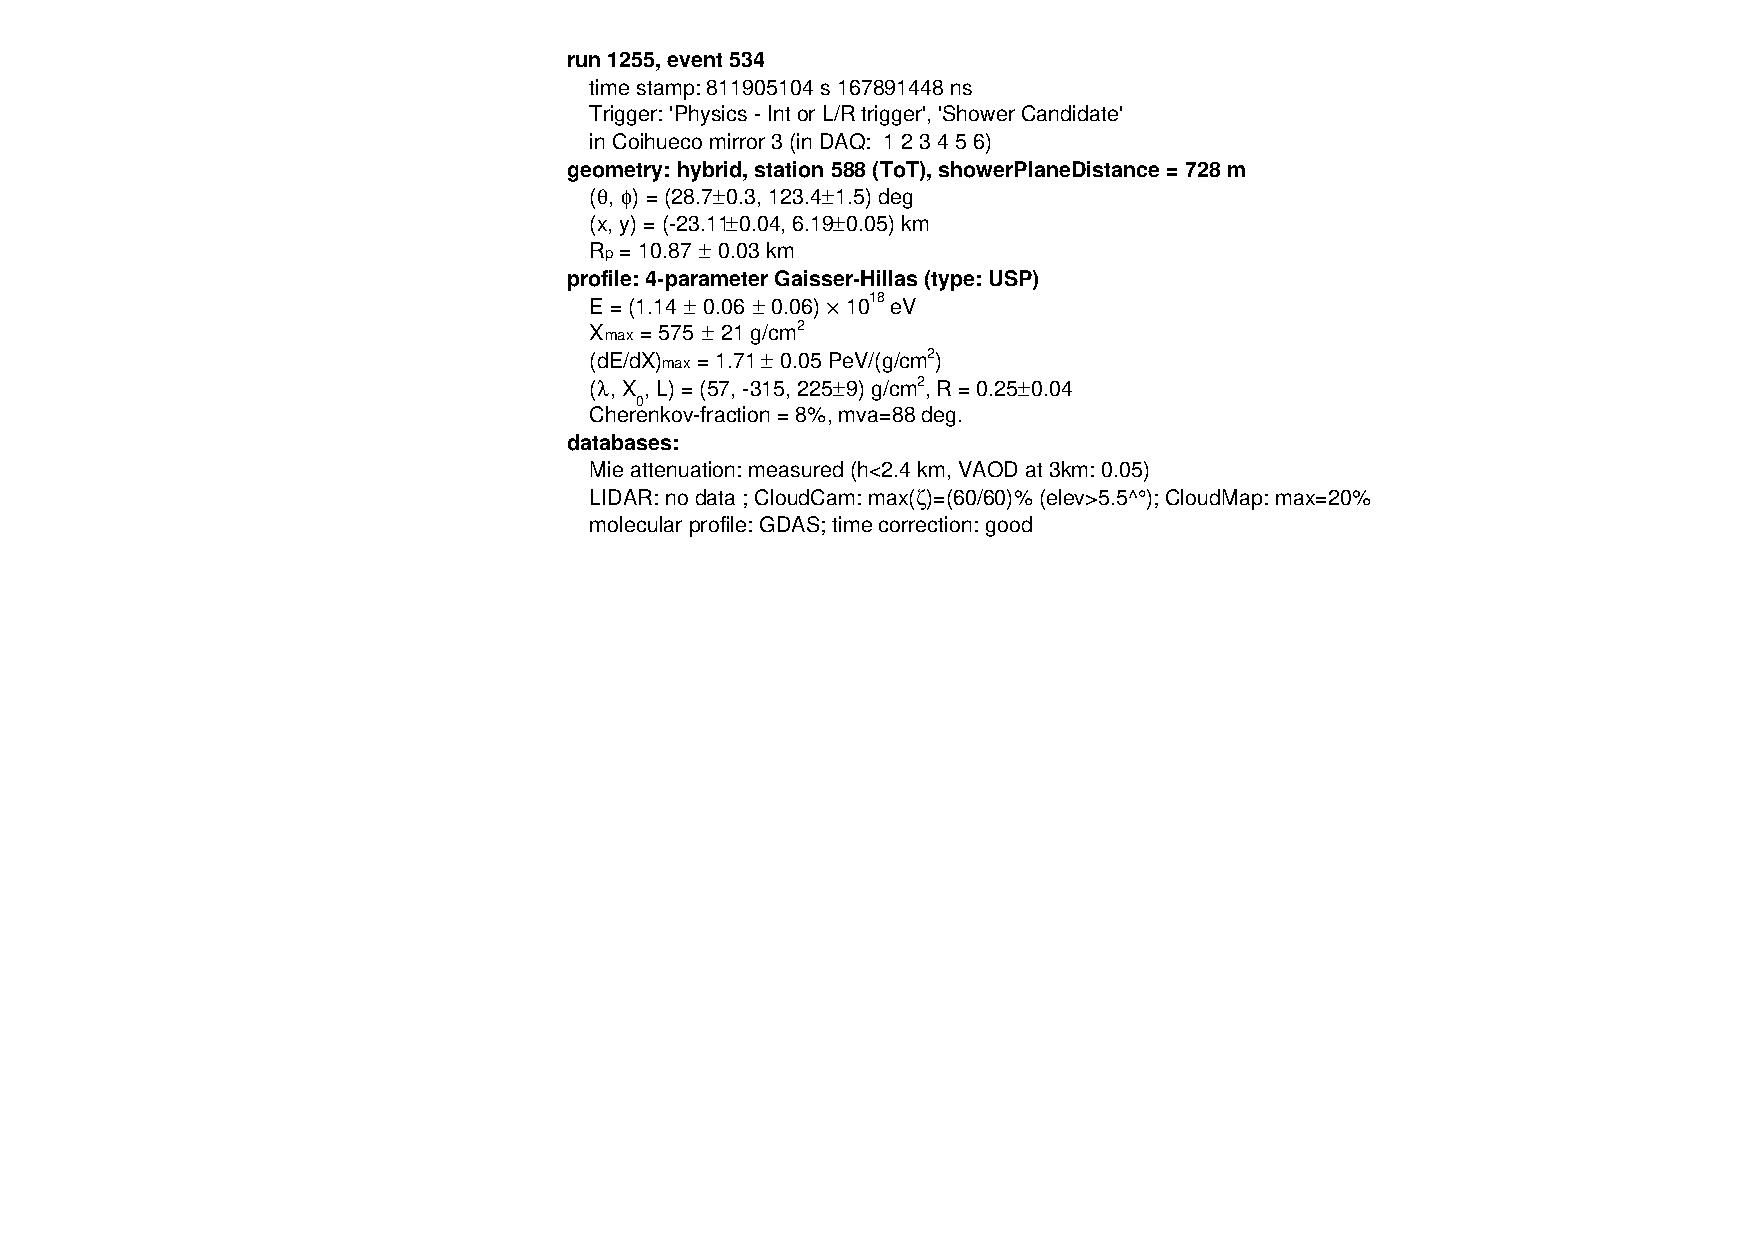
\includegraphics[width=0.45\textwidth , trim = 0 0 5.5cm 0]{/home/tsudholz/PhD/Thesis/chapters/graphs/CloudFlags/CloudCut_Events_Failed/Auger_52704749200_FdEventInfo.pdf}}
 \vspace{2cm}
  \begin{subfigure}[b]{\textwidth}
  \centering
  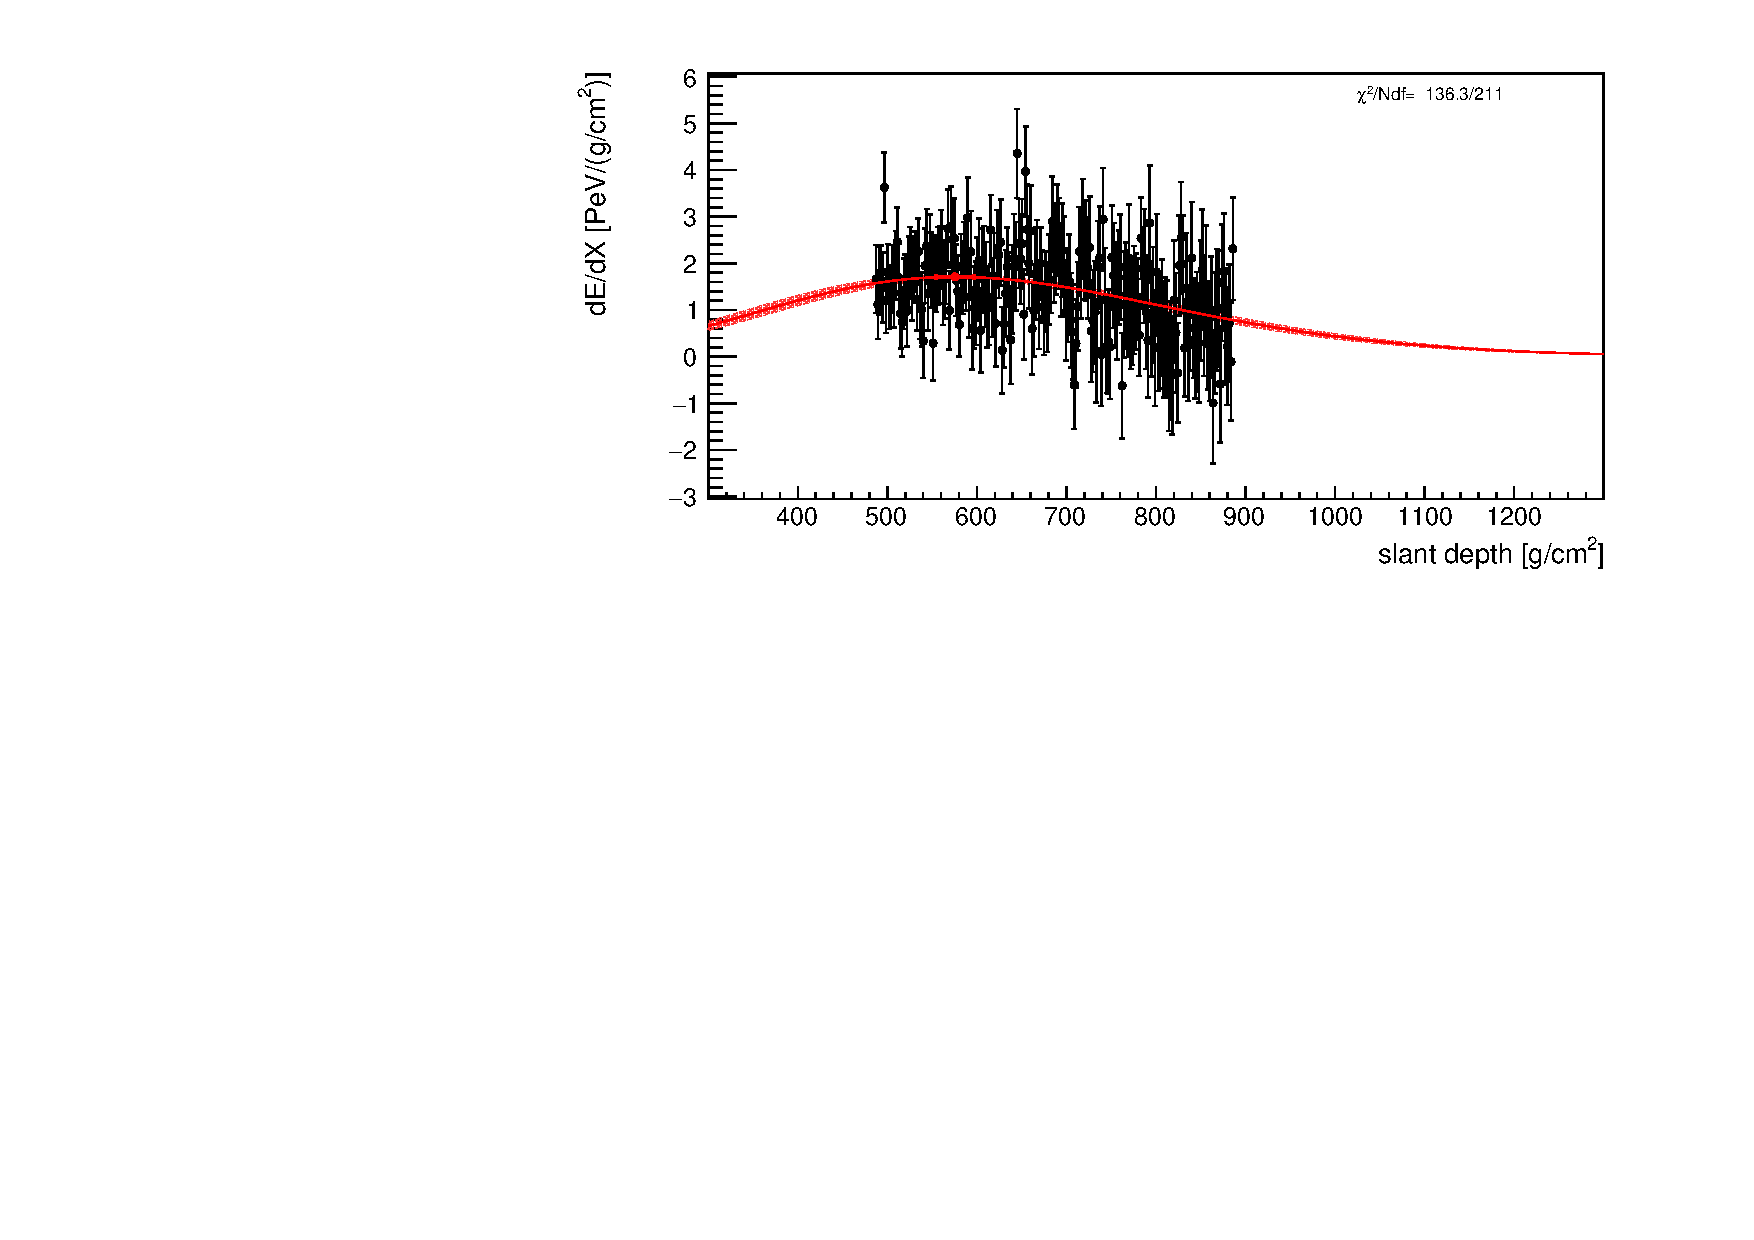
\includegraphics[width=\textwidth]{/home/tsudholz/PhD/Thesis/chapters/graphs/CloudFlags/CloudCut_Events_Failed/Auger_52704749200_SlantDepth.pdf}
  \caption{FD profile of the energy deposited as a function of atmospheric depth.}
  \end{subfigure}
 \vspace{0.5cm}
  \begin{subfigure}[b]{0.45\textwidth}
  	\centering
  	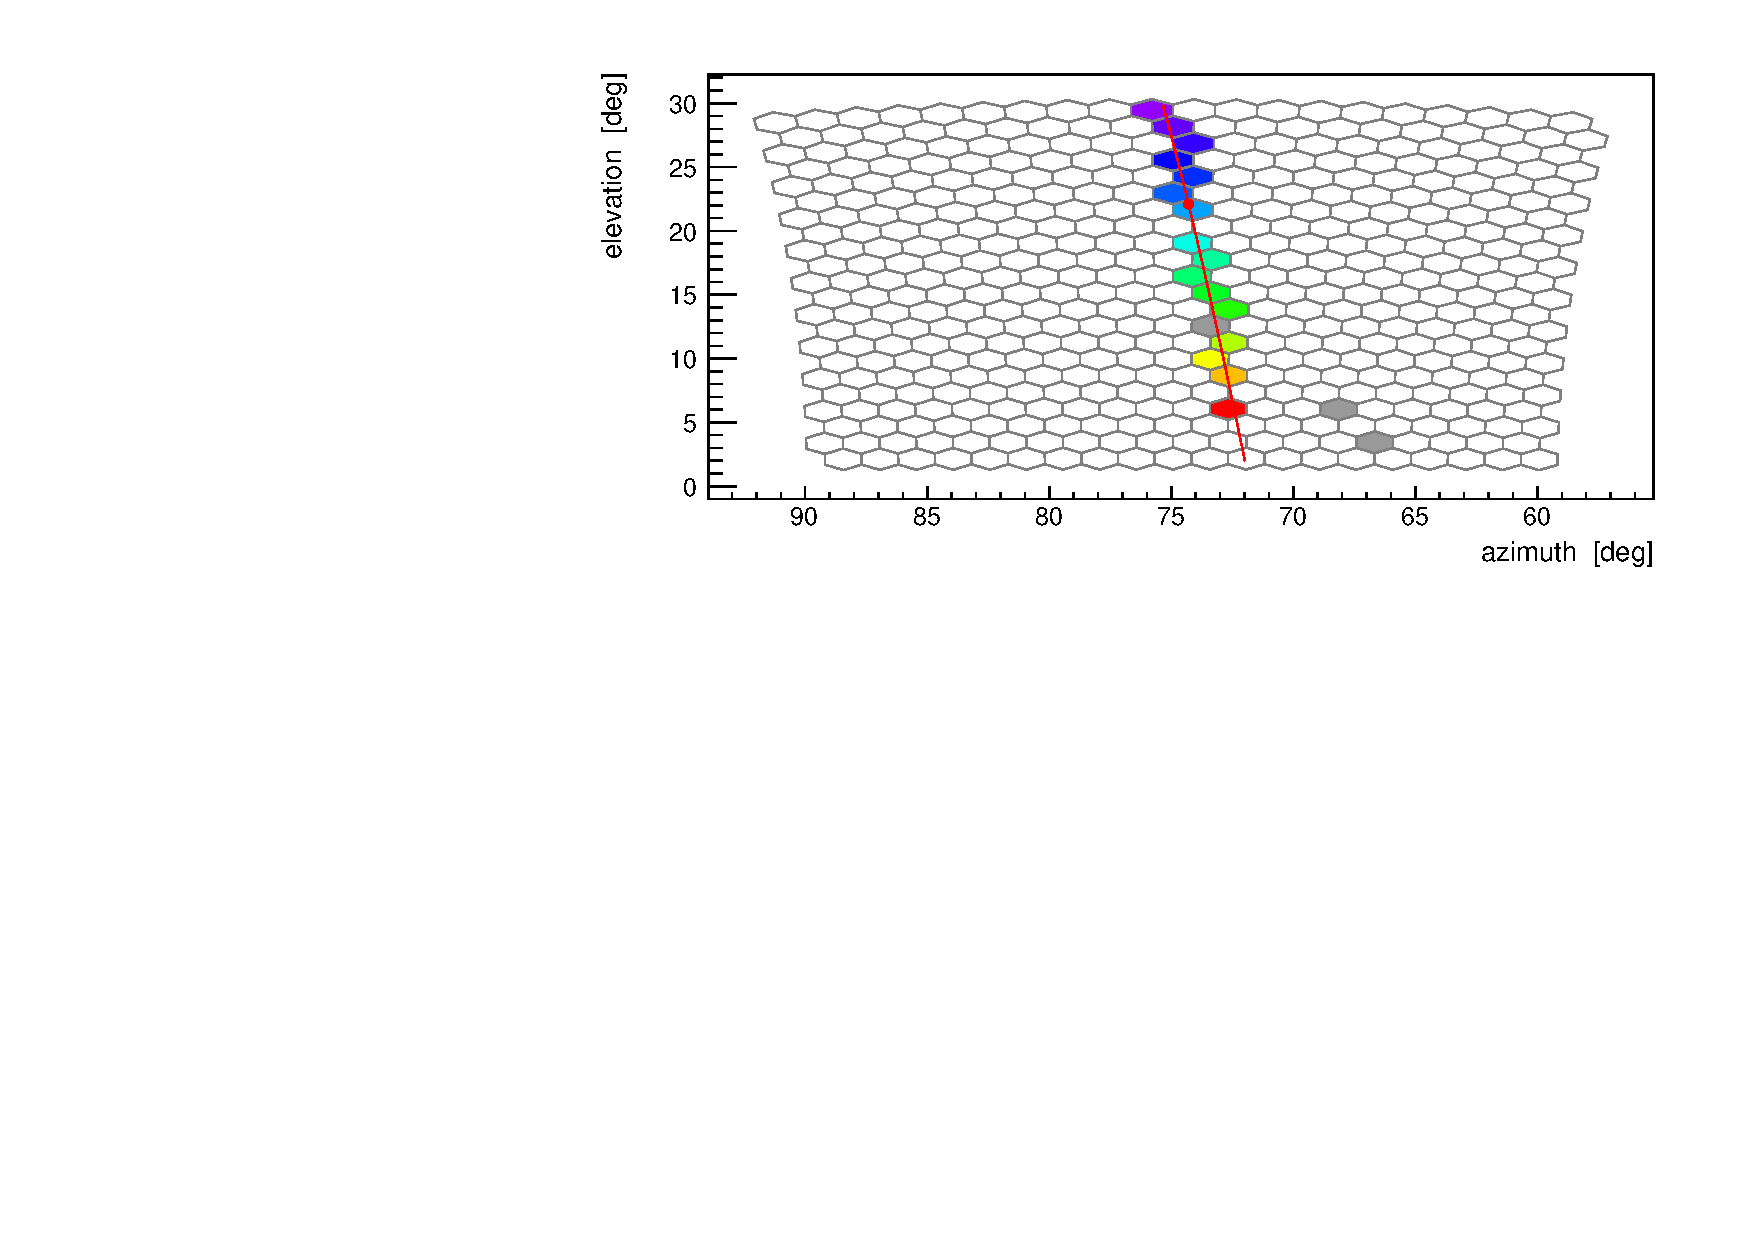
\includegraphics[width=\textwidth , height=\tempheight]{/home/tsudholz/PhD/Thesis/chapters/graphs/CloudFlags/CloudCut_Events_Failed/Auger_52704749200_FdProfile.pdf}
  	\caption{FD light profile}
  \end{subfigure}
  \begin{subfigure}[b]{0.45\textwidth}
  	\centering
  	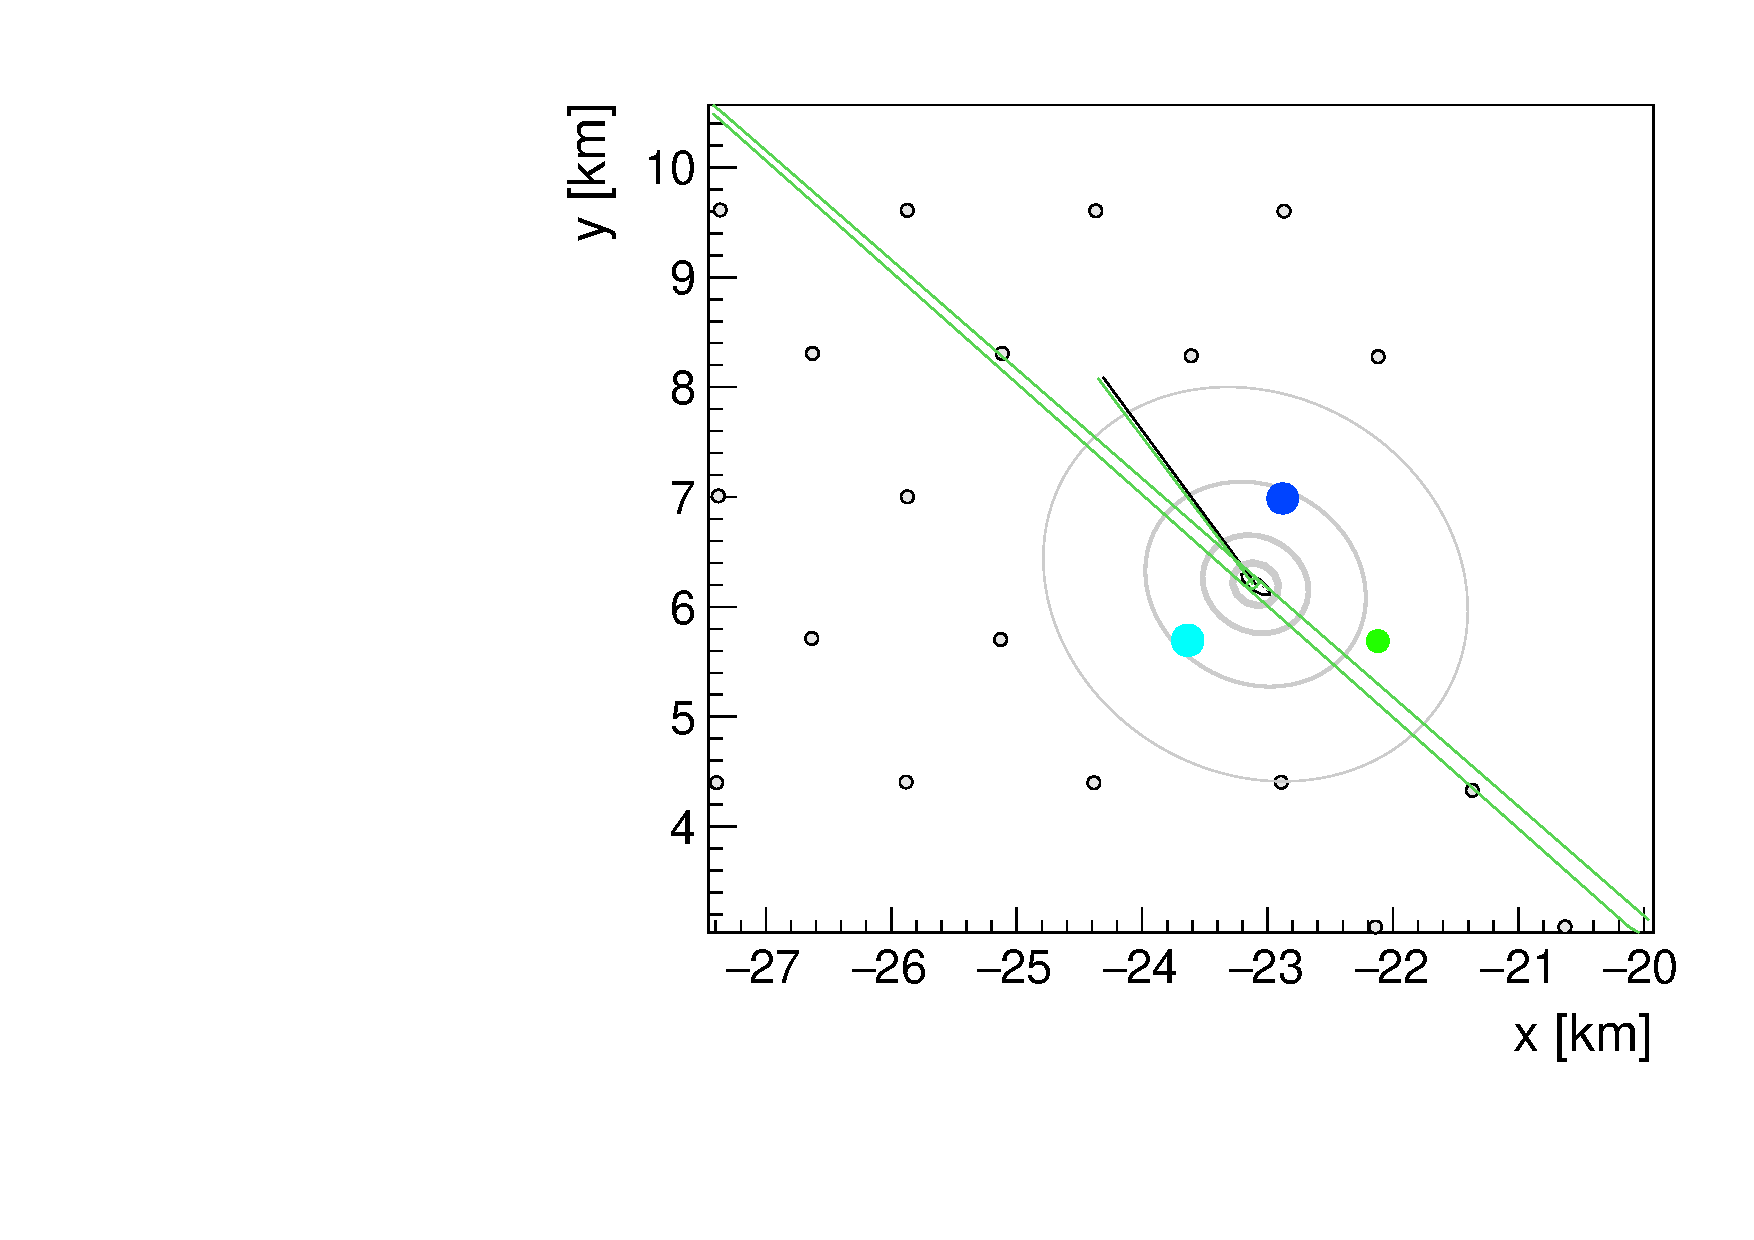
\includegraphics[width=0.8\textwidth , height=\tempheight]{/home/tsudholz/PhD/Thesis/chapters/graphs/CloudFlags/CloudCut_Events_Failed/Auger_52704749200_SdProfile.pdf}
  	\caption{SD tank triggered profile}
  \end{subfigure}

  \begin{subfigure}[b]{0.45\textwidth}
  	\centering
	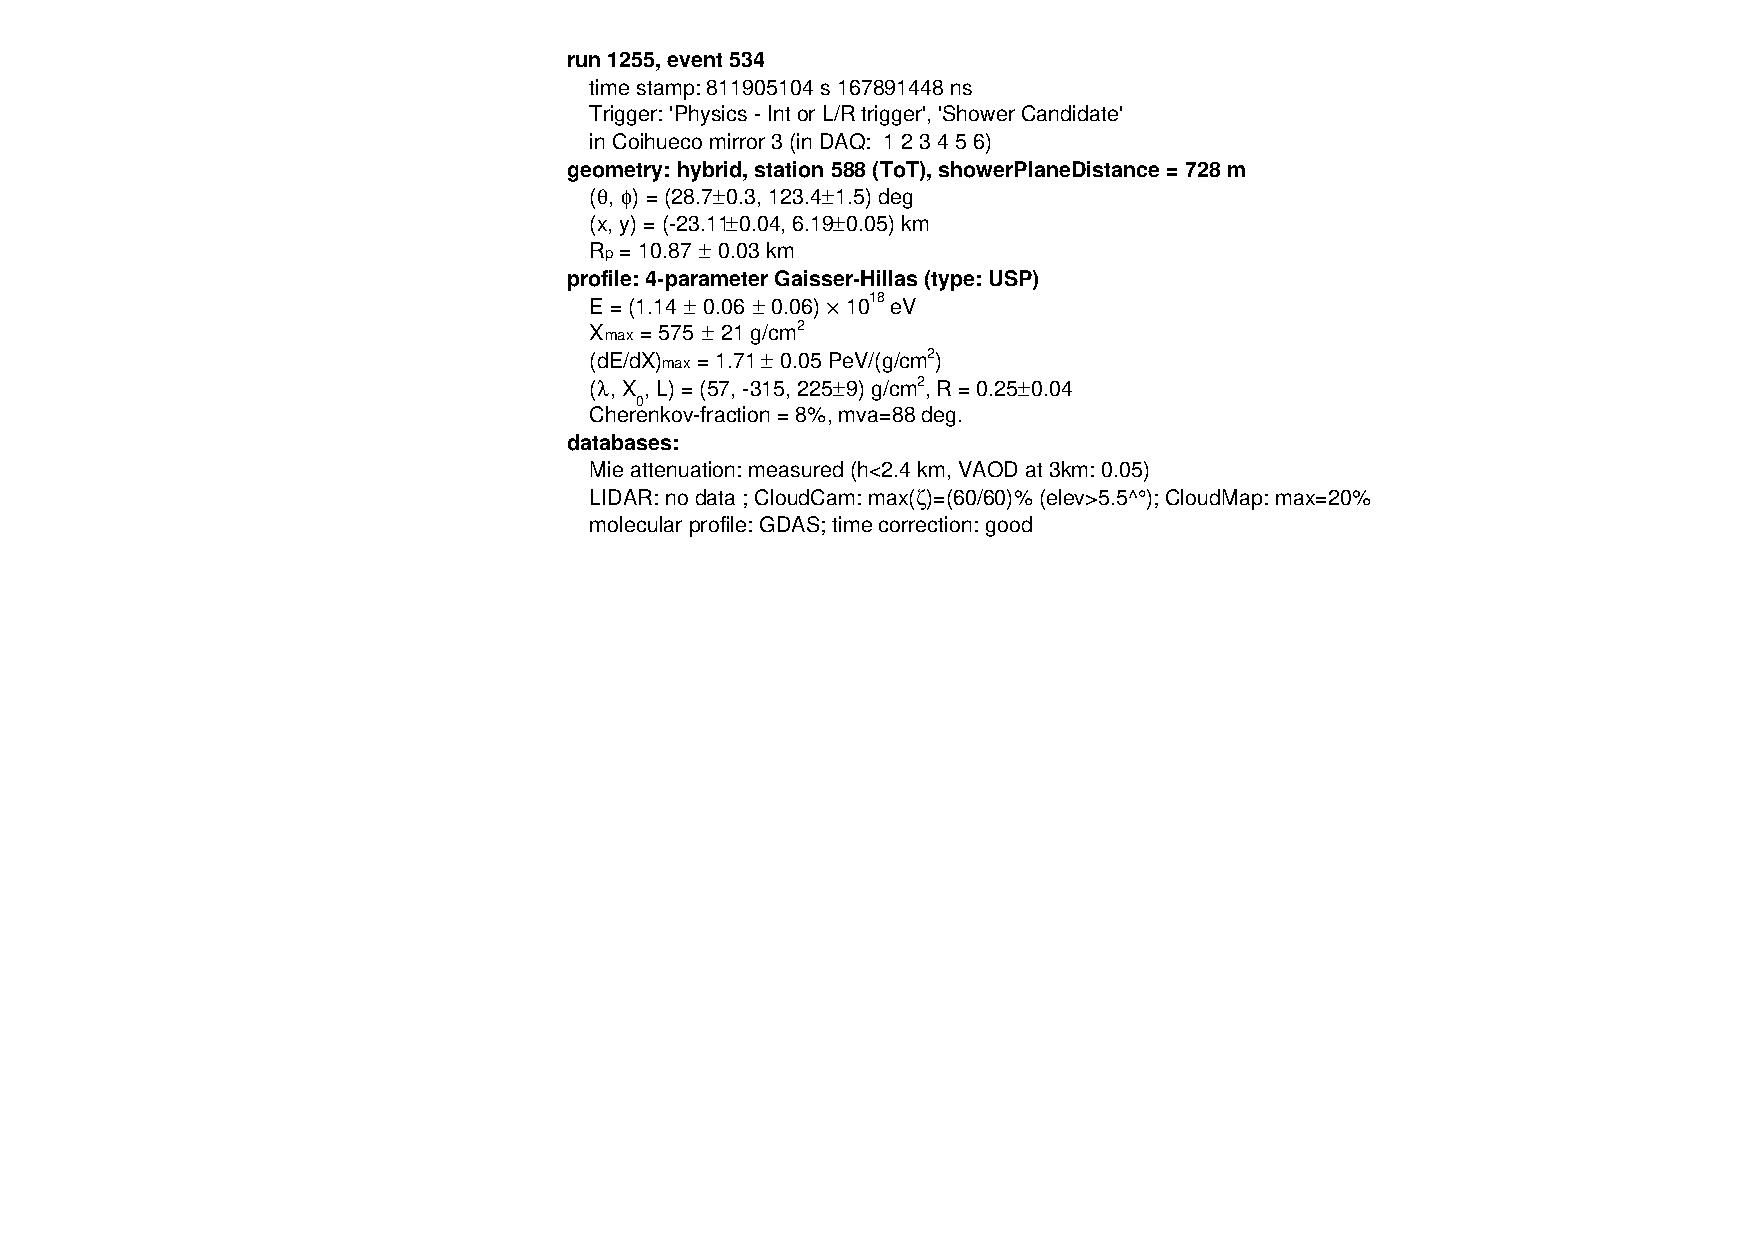
\includegraphics[height=\tempheight , trim = 0 0 5.5cm 0]{/home/tsudholz/PhD/Thesis/chapters/graphs/CloudFlags/CloudCut_Events_Failed/Auger_52704749200_FdEventInfo.pdf}
  	\caption{FD light profile}
  \end{subfigure}
  \begin{subfigure}[b]{0.45\textwidth}
  	\centering
	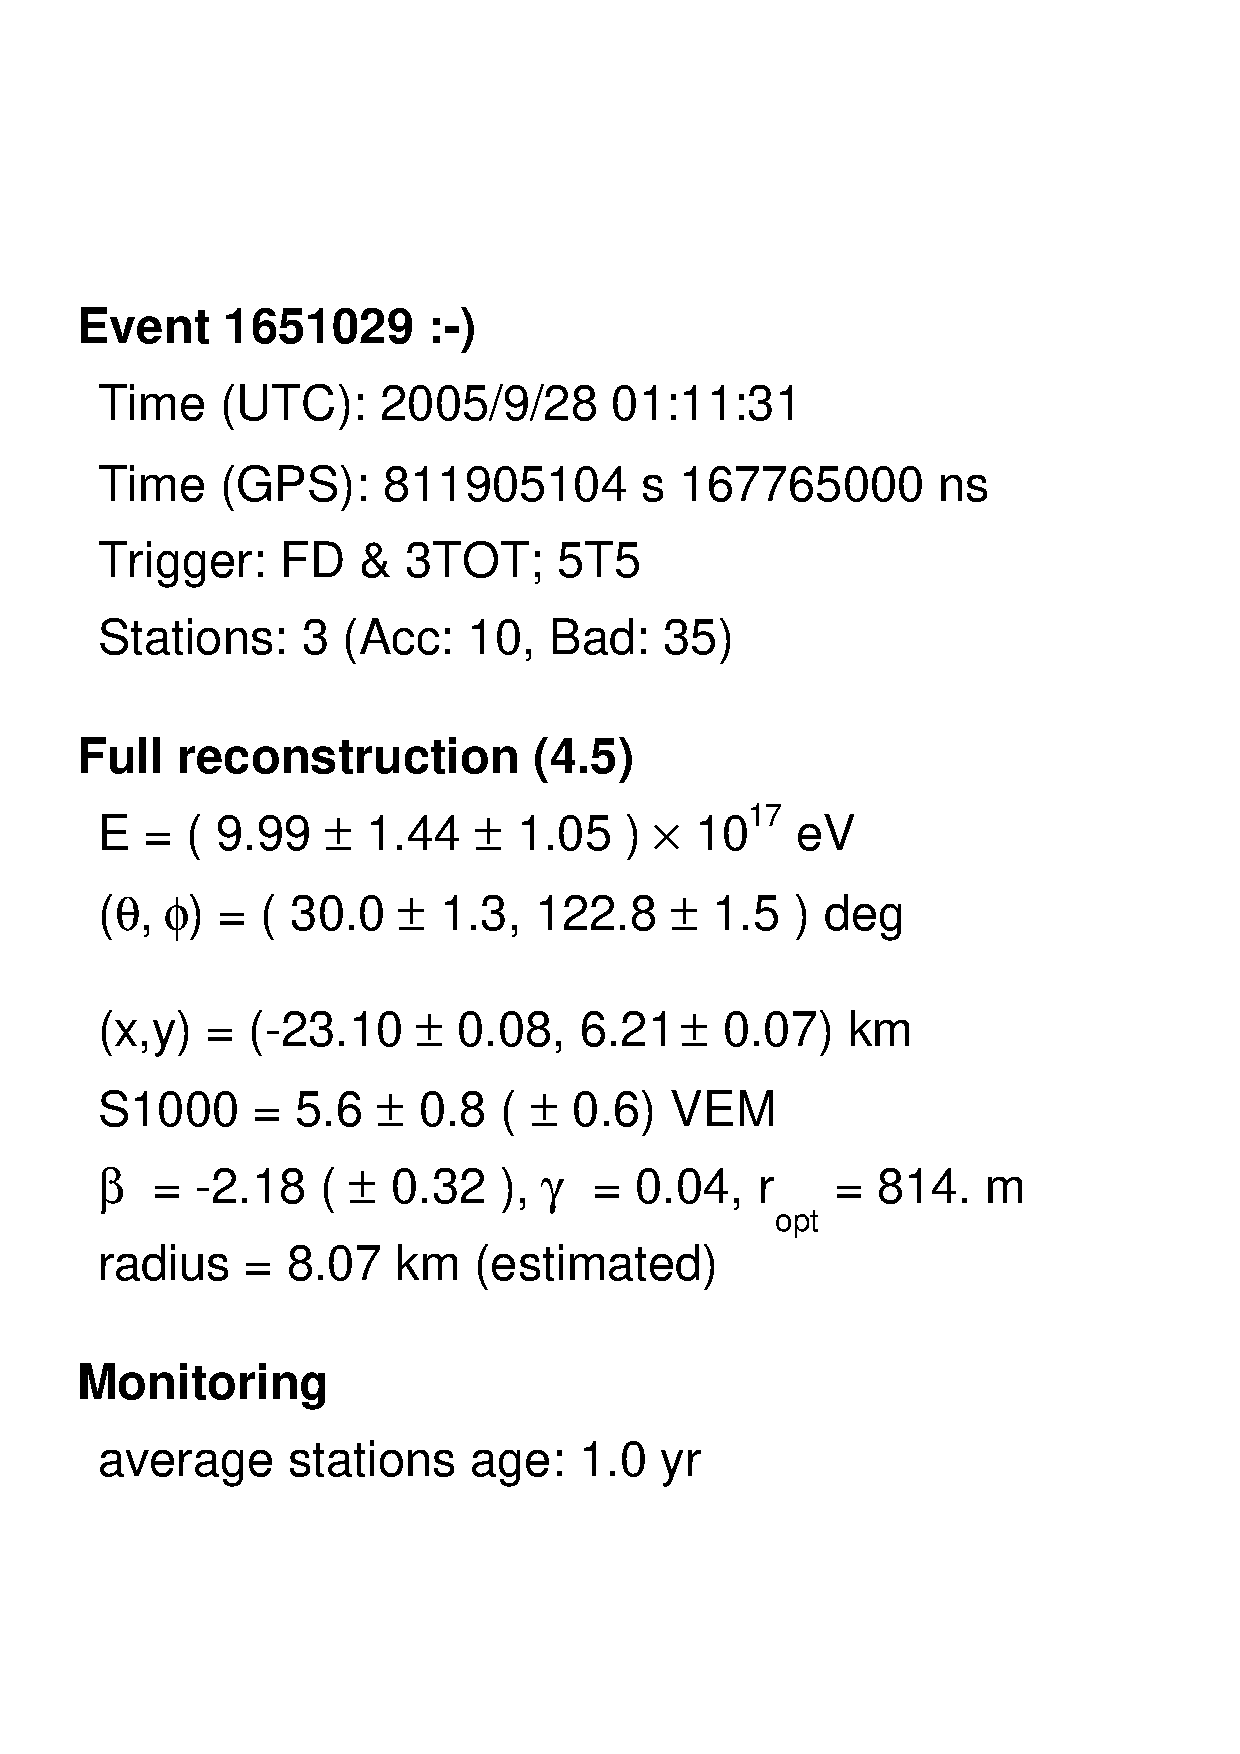
\includegraphics[height=\tempheight]{/home/tsudholz/PhD/Thesis/chapters/graphs/CloudFlags/CloudCut_Events_Failed/Auger_52704749200_SdEventInfo.pdf}
  	\caption{SD tank triggered profile}
  \end{subfigure}
  \caption{Example of an Auger event that would fail the cloud selection cut from EventBrowser}
\end{figure}

\begin{figure}
\centering
  \settoheight{\tempheight}{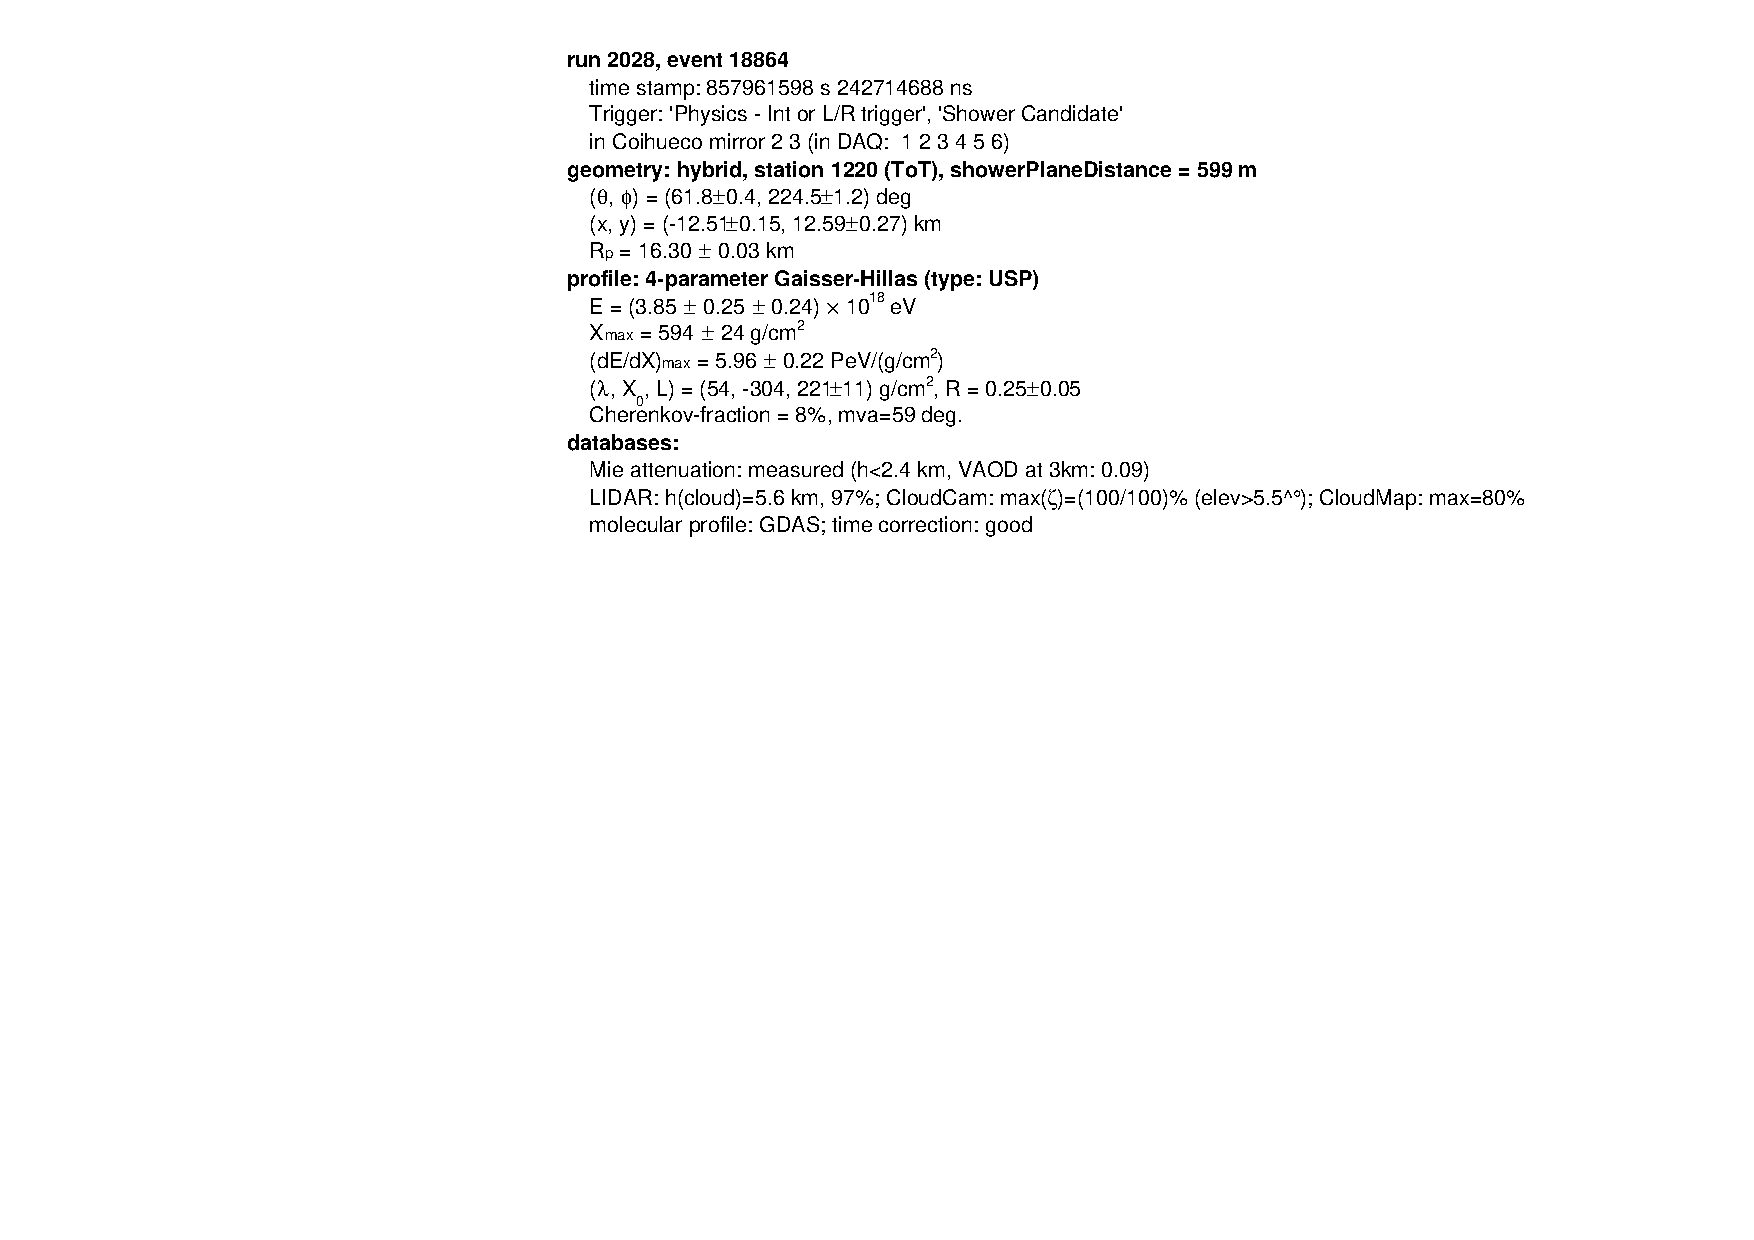
\includegraphics[width=0.45\textwidth , trim = 0 0 5.5cm 0]{/home/tsudholz/PhD/Thesis/chapters/graphs/CloudFlags/CloudCut_Events_Failed/Auger_70735278500_FdEventInfo.pdf}}
 \vspace{2cm}
  \begin{subfigure}[b]{\textwidth}
  \centering
  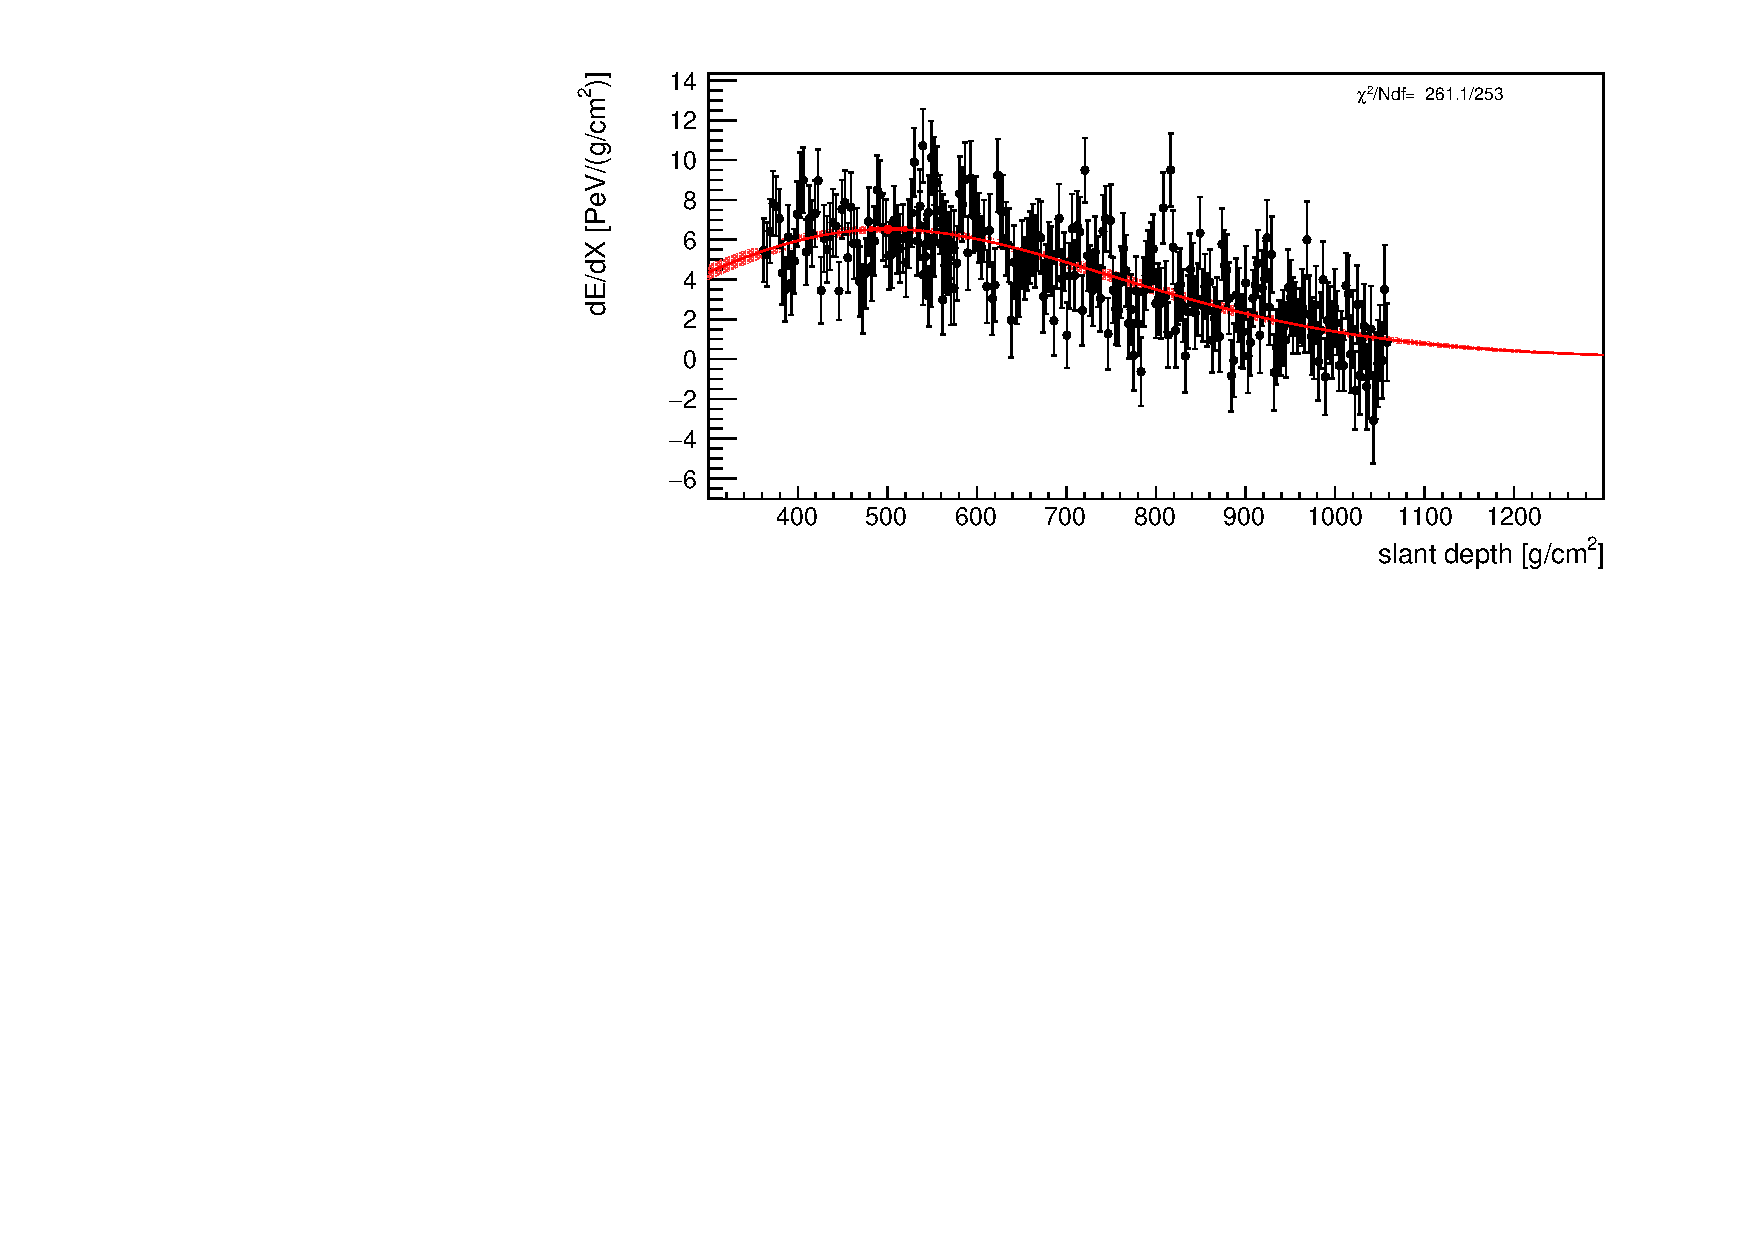
\includegraphics[width=\textwidth]{/home/tsudholz/PhD/Thesis/chapters/graphs/CloudFlags/CloudCut_Events_Failed/Auger_160416430001_SlantDepth.pdf}
  \caption{FD profile of the energy deposited as a function of atmospheric depth.}
  \end{subfigure}
 \vspace{0.5cm}
  \begin{subfigure}[b]{0.45\textwidth}
  	\centering
  	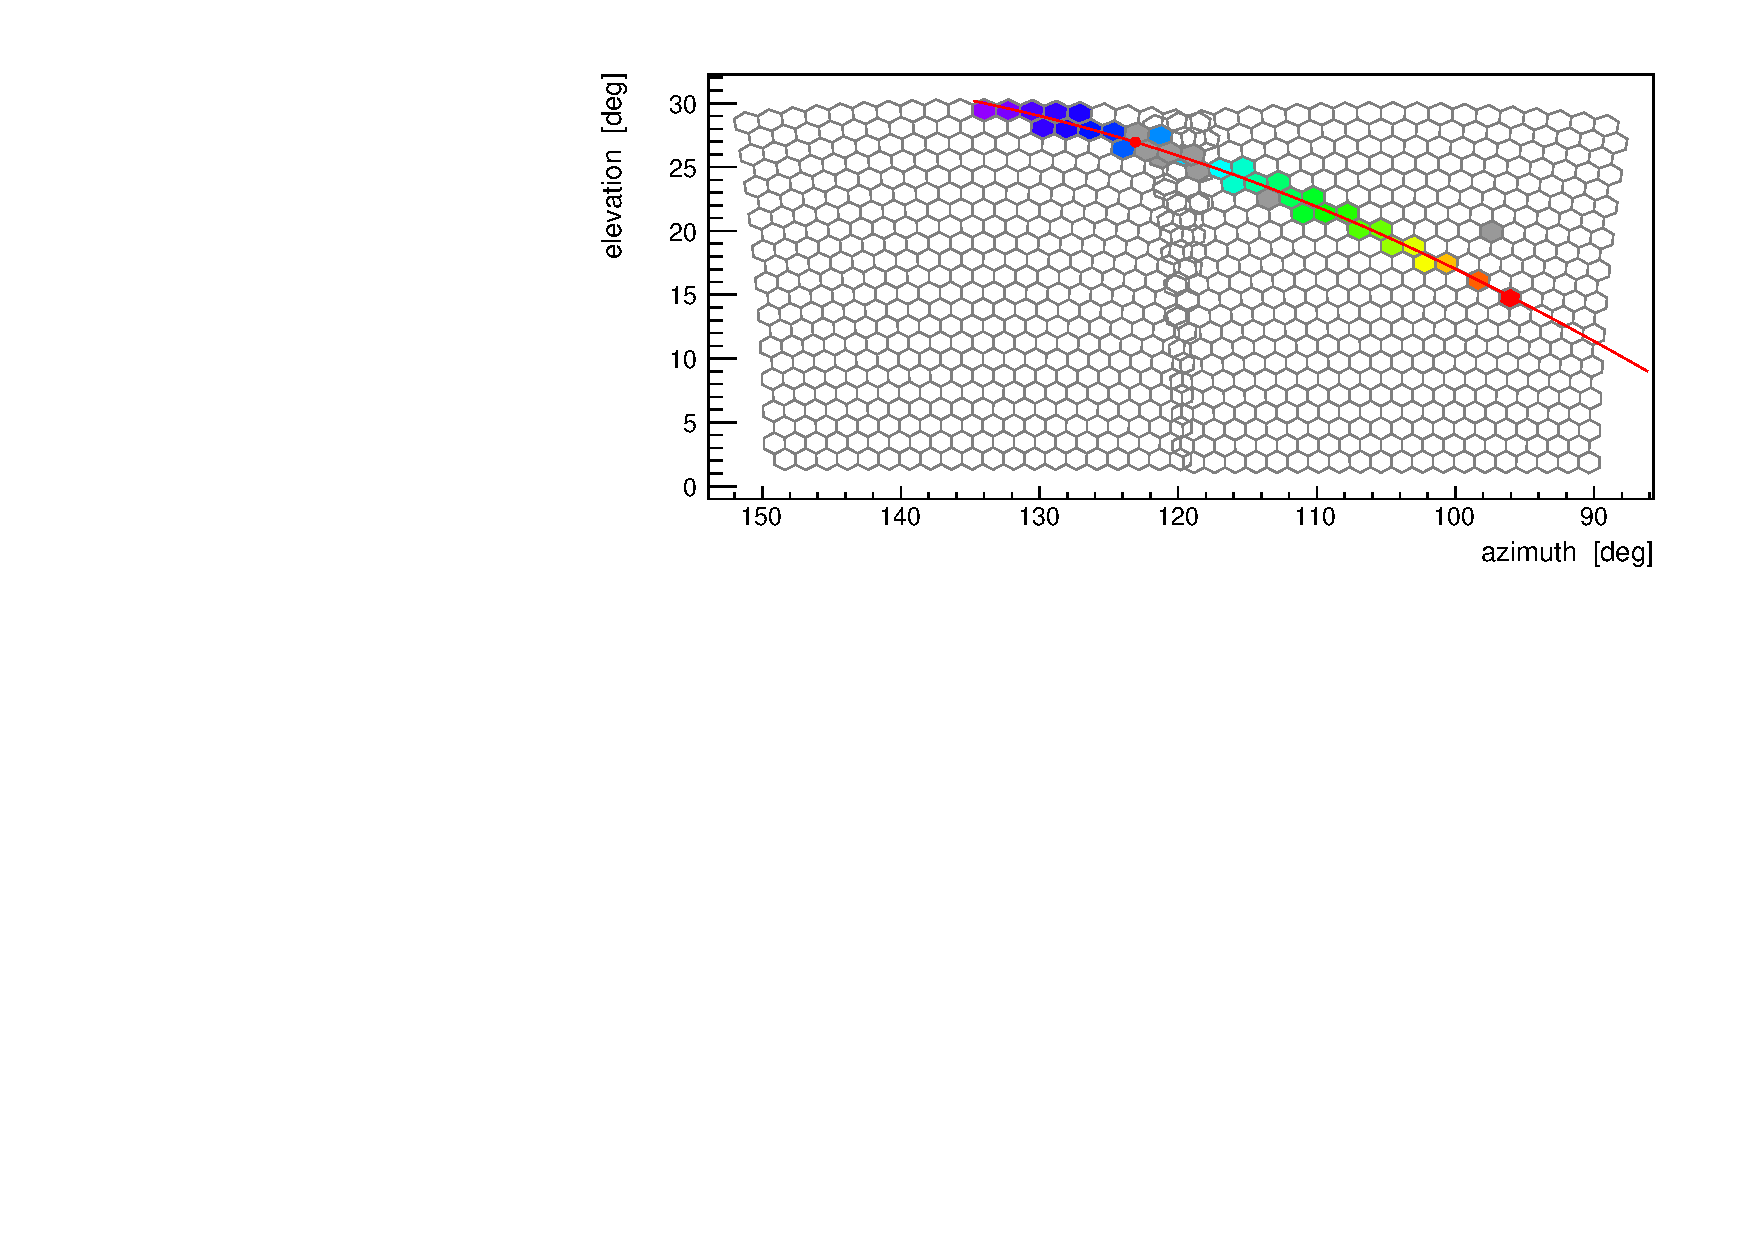
\includegraphics[width=\textwidth , height=\tempheight]{/home/tsudholz/PhD/Thesis/chapters/graphs/CloudFlags/CloudCut_Events_Failed/Auger_160416430001_FdProfile.pdf}
  	\caption{FD light profile}
  \end{subfigure}
  \begin{subfigure}[b]{0.45\textwidth}
  	\centering
  	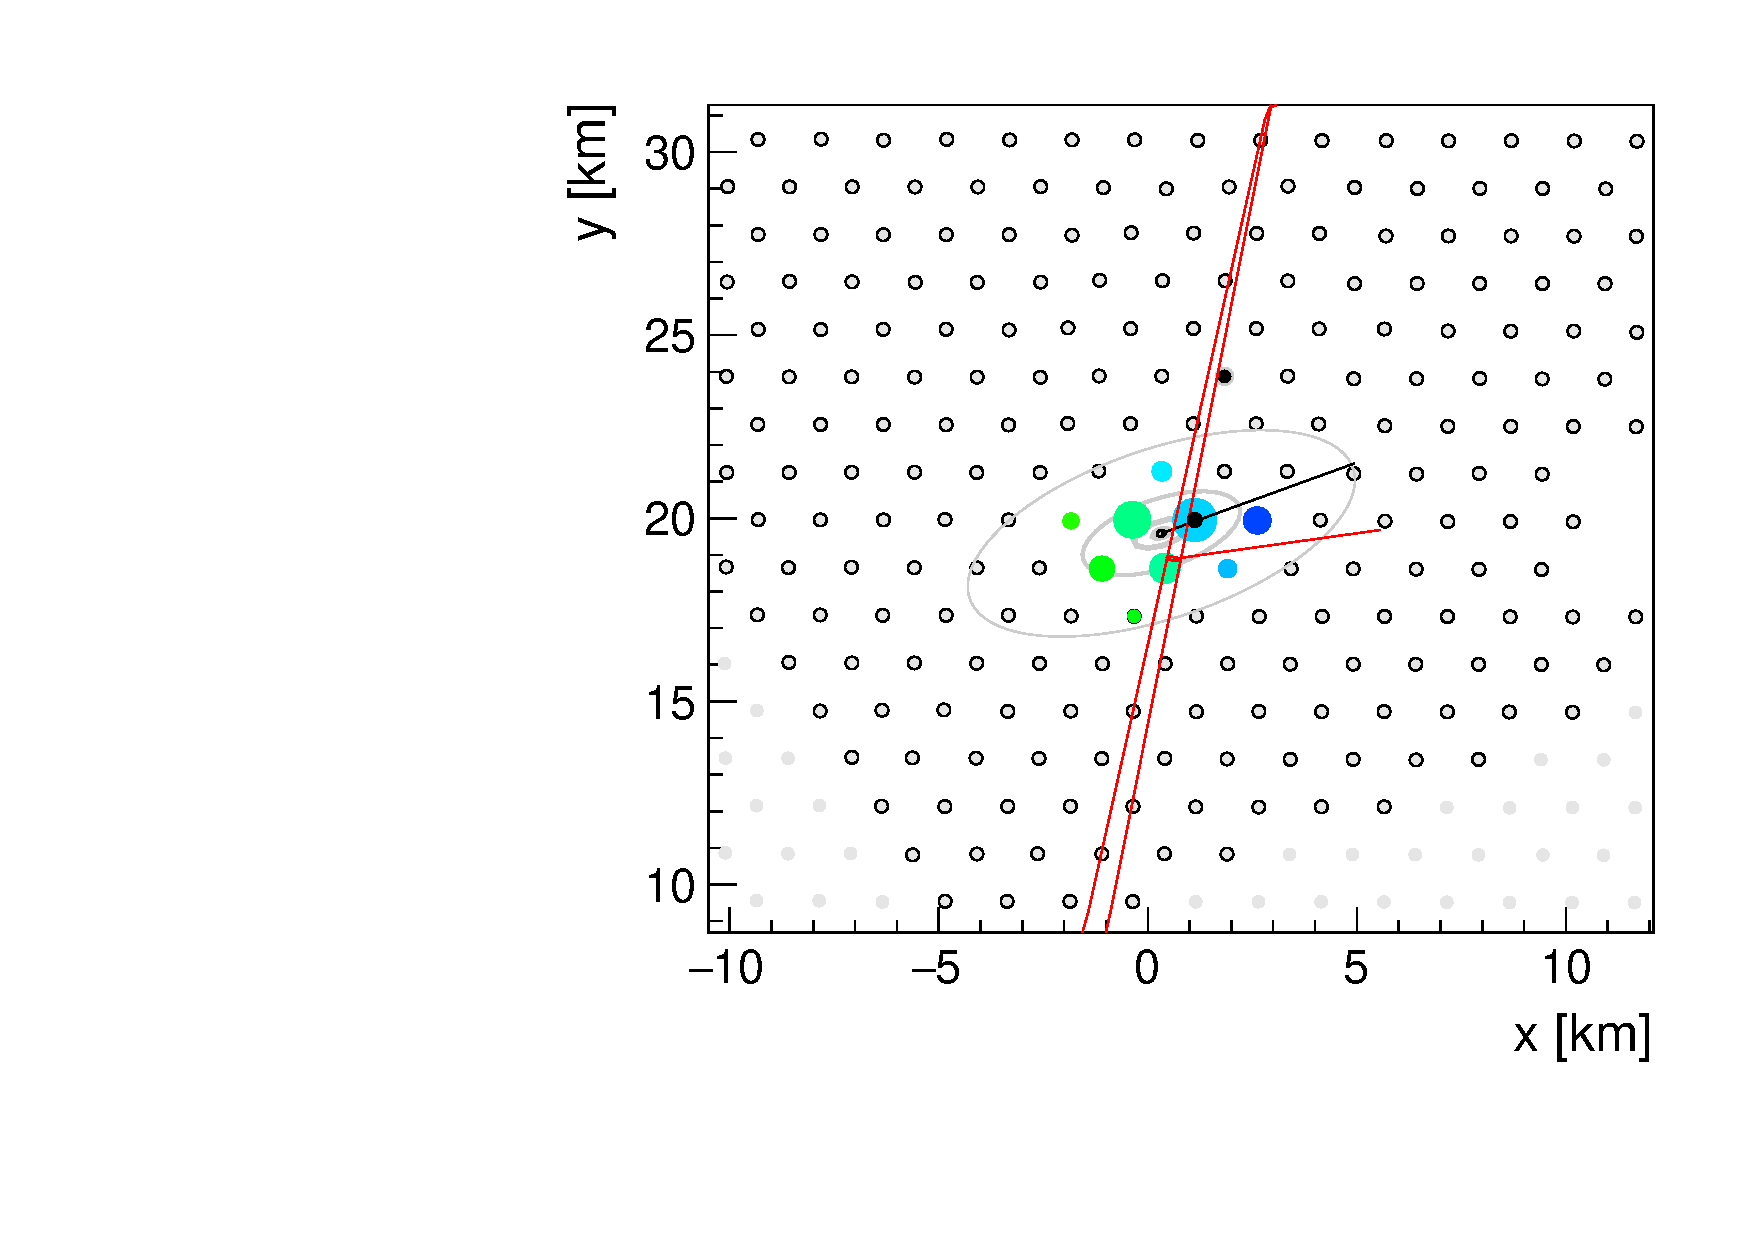
\includegraphics[width=0.8\textwidth , height=\tempheight]{/home/tsudholz/PhD/Thesis/chapters/graphs/CloudFlags/CloudCut_Events_Failed/Auger_160416430001_SdProfile.pdf}
  	\caption{SD tank triggered profile}
  \end{subfigure}

  \begin{subfigure}[b]{0.45\textwidth}
  	\centering
	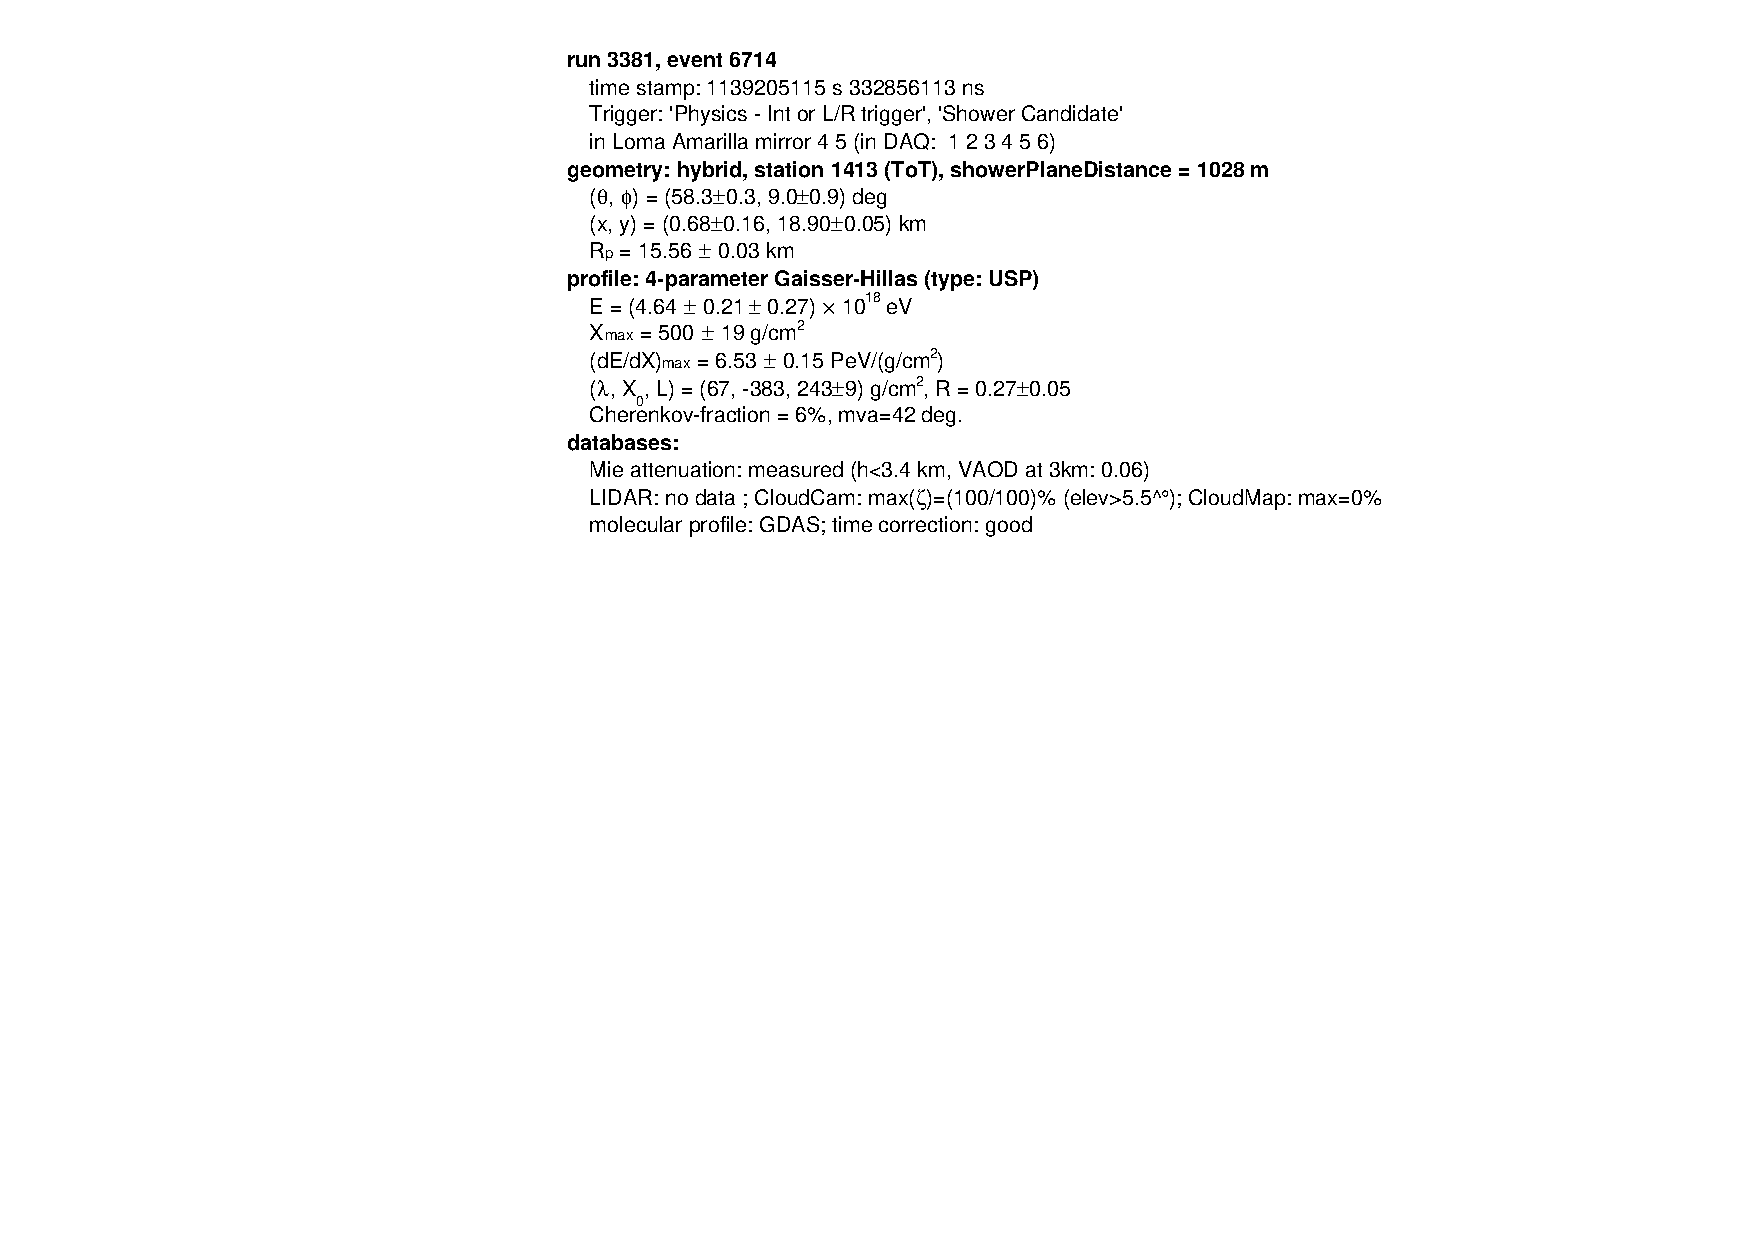
\includegraphics[height=\tempheight , trim = 0 0 5.5cm 0]{/home/tsudholz/PhD/Thesis/chapters/graphs/CloudFlags/CloudCut_Events_Failed/Auger_160416430001_FdEventInfo.pdf}
  	\caption{FD light profile}
  \end{subfigure}
  \begin{subfigure}[b]{0.45\textwidth}
  	\centering
	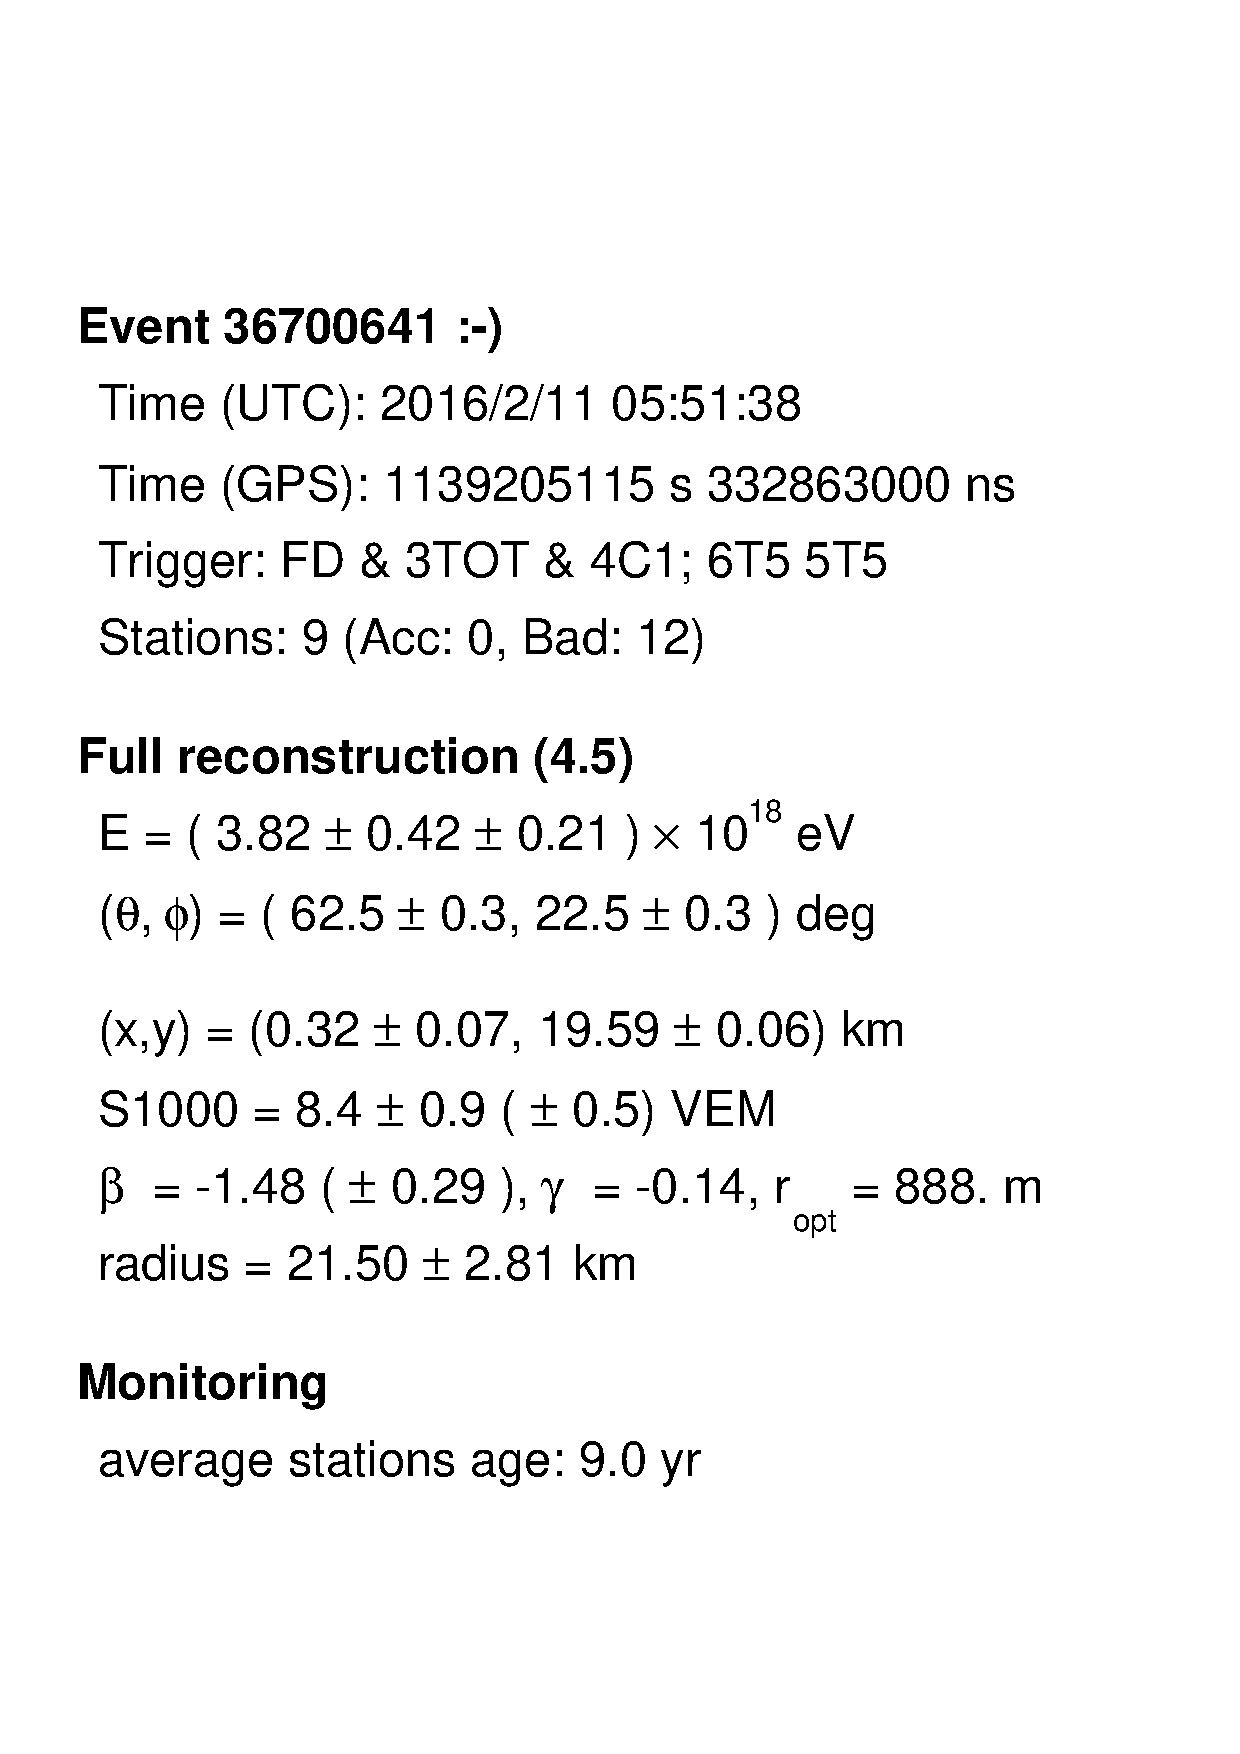
\includegraphics[height=\tempheight]{/home/tsudholz/PhD/Thesis/chapters/graphs/CloudFlags/CloudCut_Events_Failed/Auger_160416430001_SdEventInfo.pdf}
  	\caption{SD tank triggered profile}
  \end{subfigure}
  \caption{Example of an Auger event that would fail the cloud selection cut from EventBrowser}
\end{figure}

\begin{figure}
\centering
  \settoheight{\tempheight}{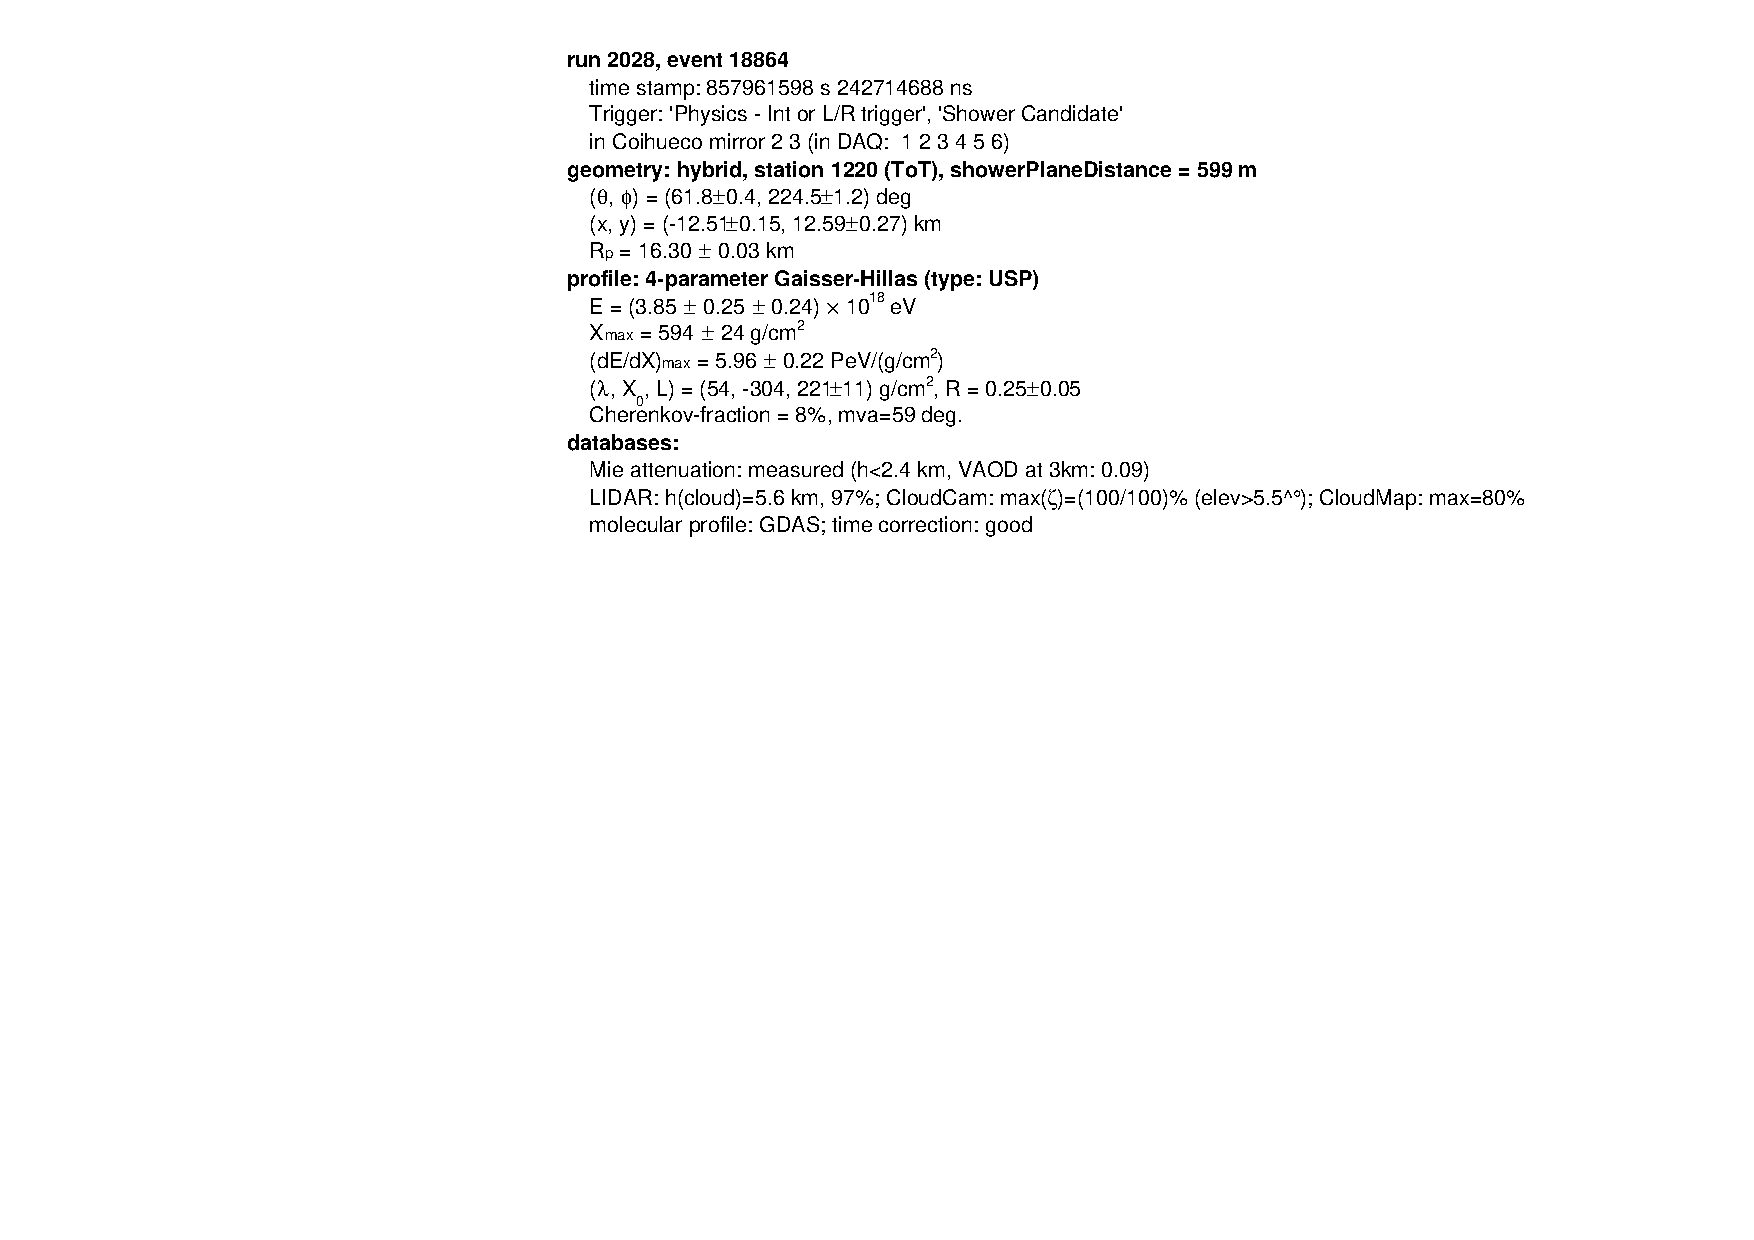
\includegraphics[width=0.45\textwidth , trim = 0 0 5.5cm 0]{/home/tsudholz/PhD/Thesis/chapters/graphs/CloudFlags/CloudCut_Events_Failed/Auger_70735278500_FdEventInfo.pdf}}
 \vspace{2cm}
  \begin{subfigure}[b]{\textwidth}
  \centering
  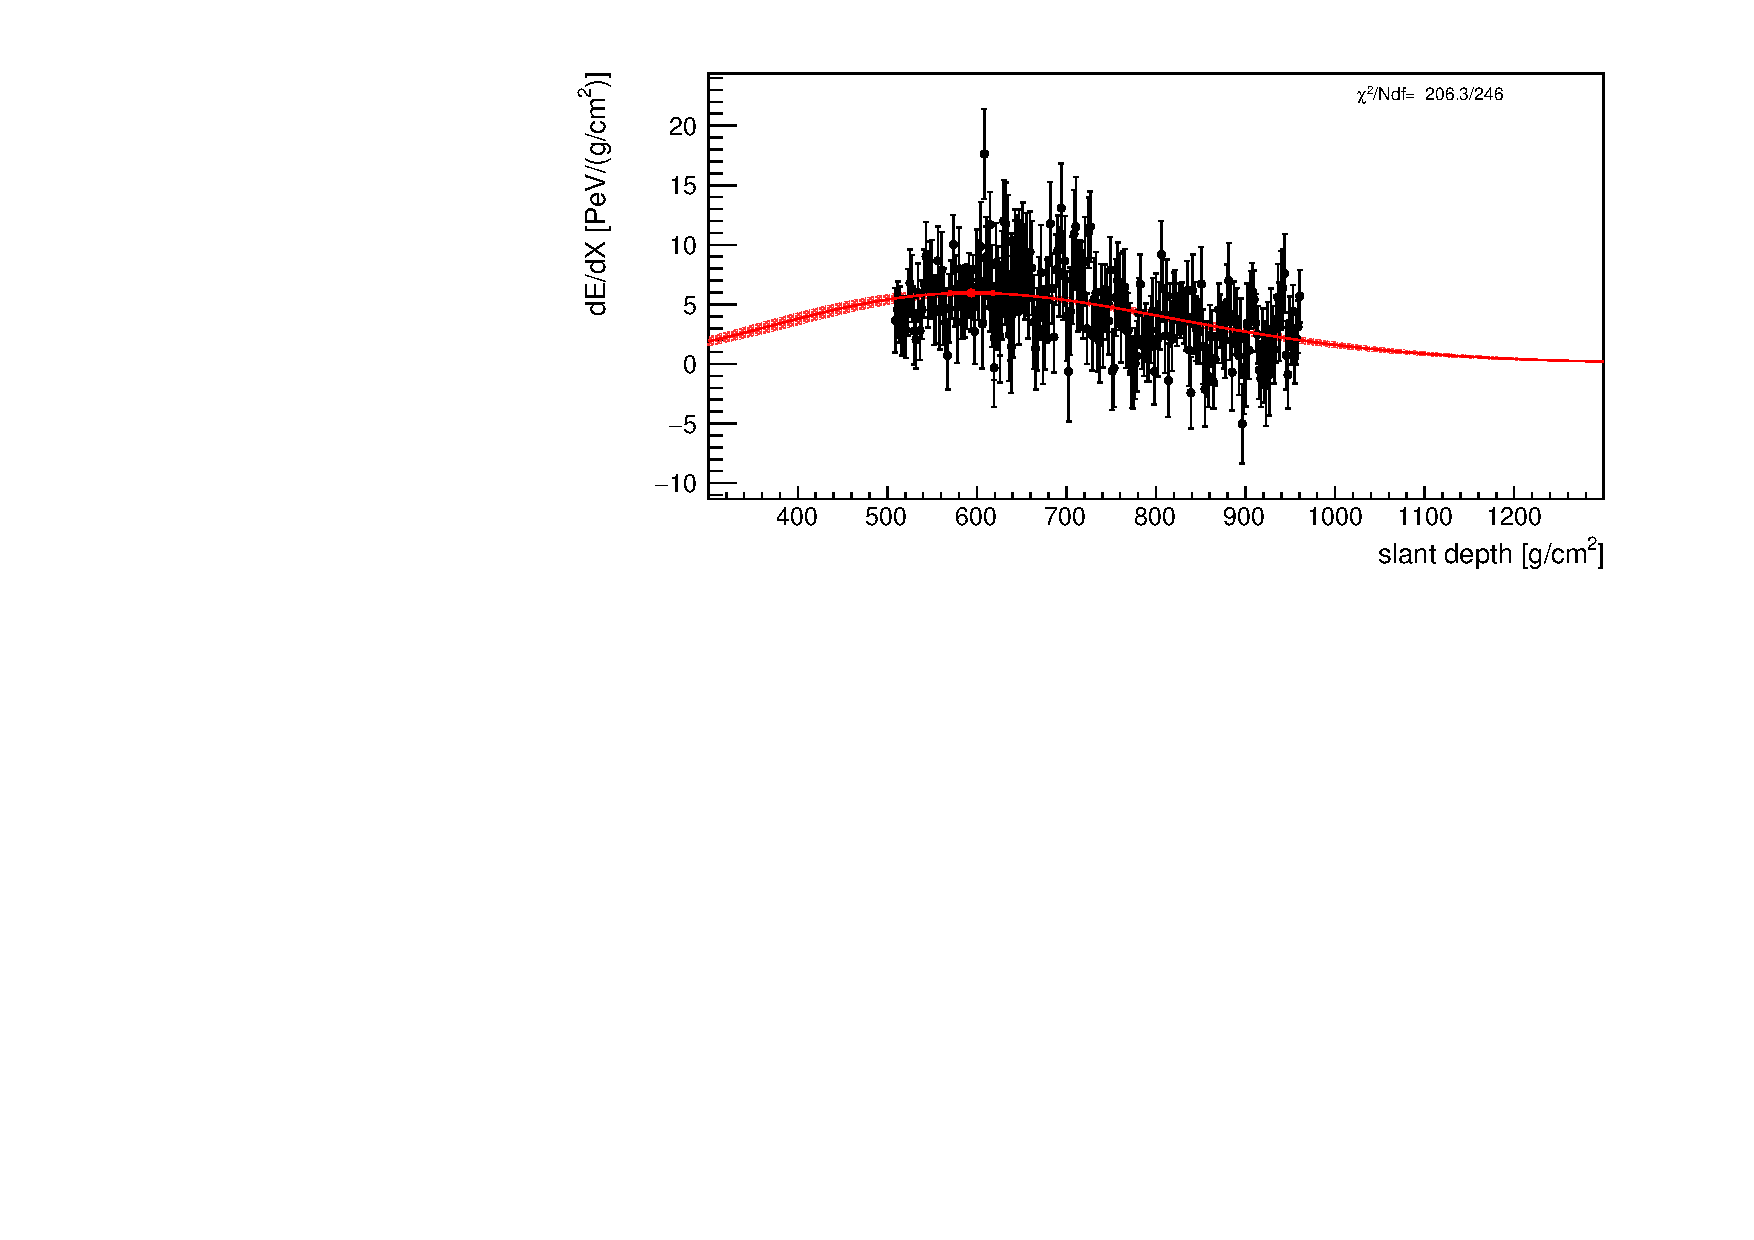
\includegraphics[width=\textwidth]{/home/tsudholz/PhD/Thesis/chapters/graphs/CloudFlags/CloudCut_Events_Failed/Auger_70735278500_SlantDepth.pdf}
  \caption{FD profile of the energy deposited as a function of atmospheric depth.}
  \end{subfigure}
 \vspace{0.5cm}
  \begin{subfigure}[b]{0.45\textwidth}
  	\centering
  	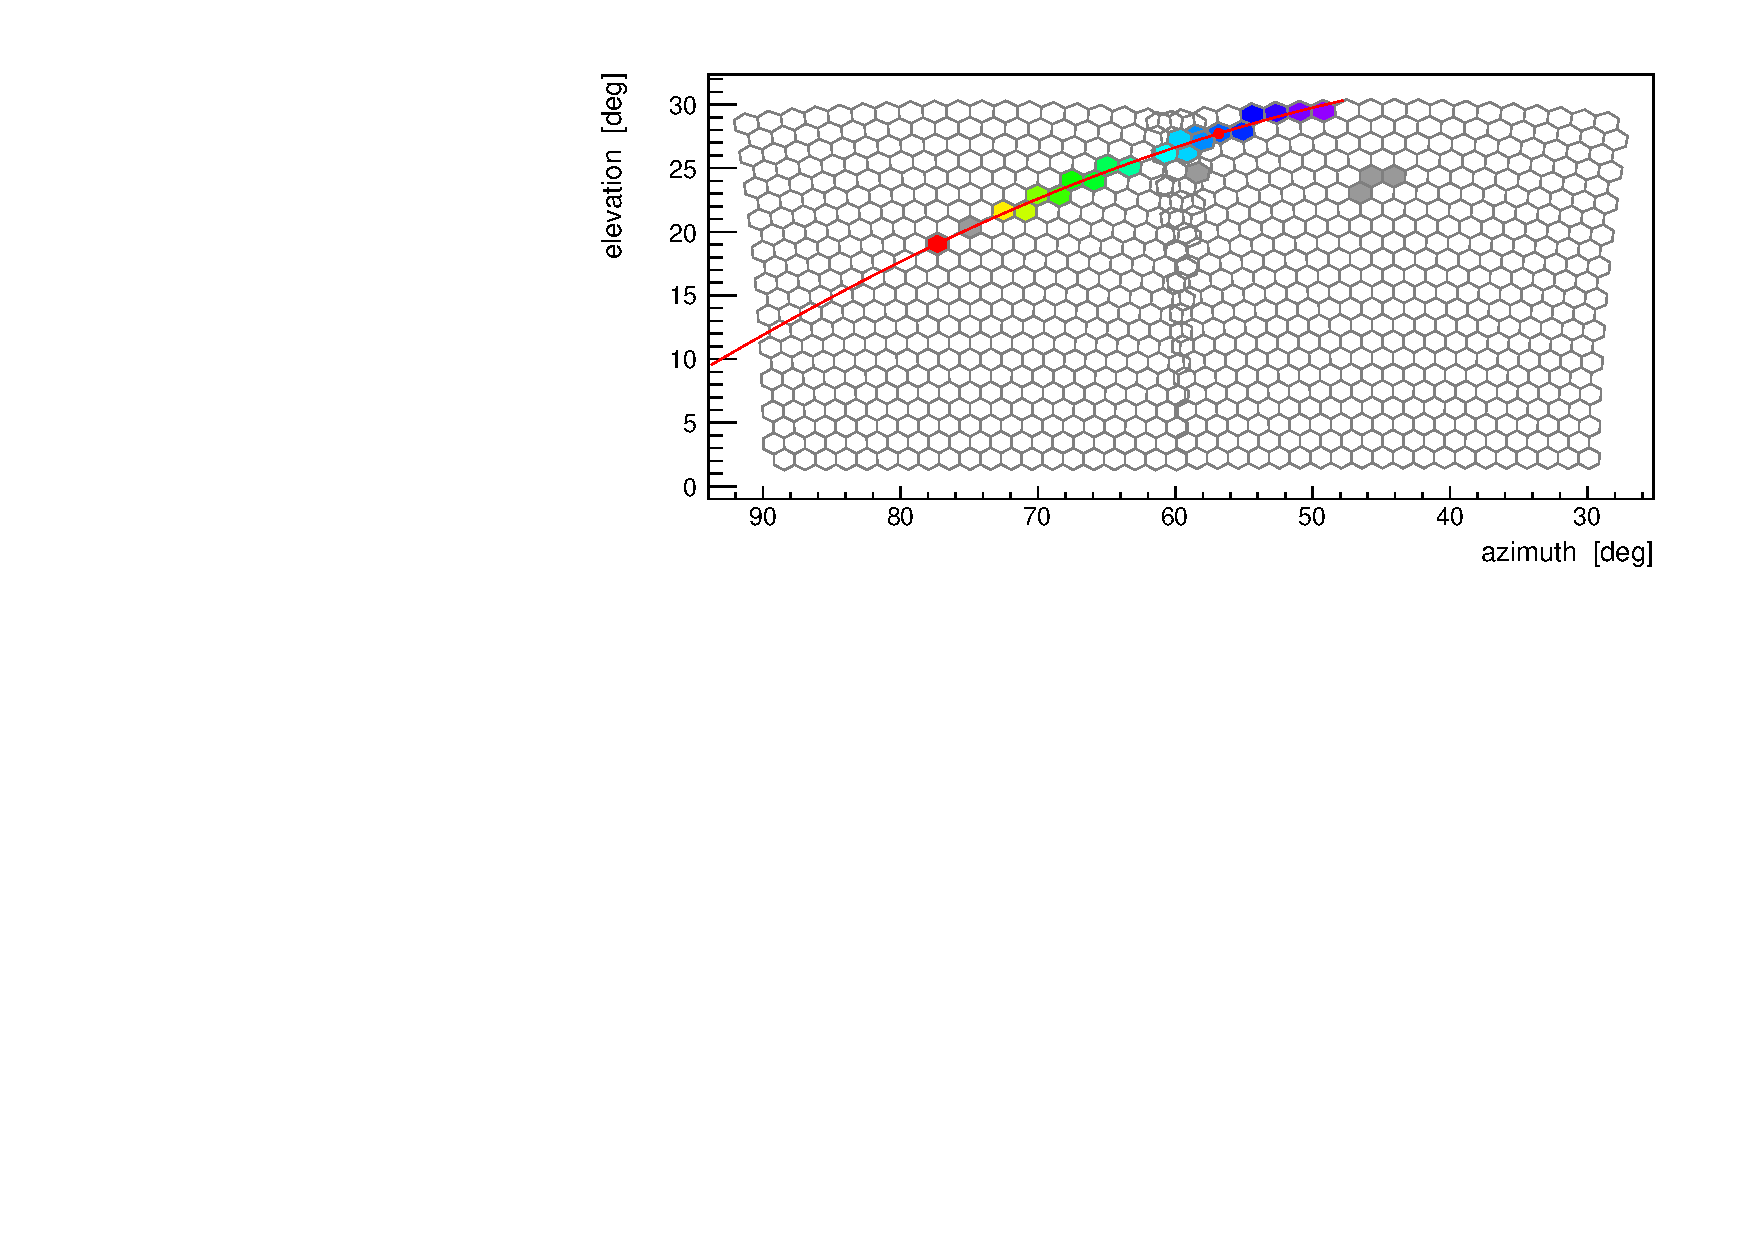
\includegraphics[width=\textwidth , height=\tempheight]{/home/tsudholz/PhD/Thesis/chapters/graphs/CloudFlags/CloudCut_Events_Failed/Auger_70735278500_FdProfile.pdf}
  	\caption{FD light profile}
  \end{subfigure}
  \begin{subfigure}[b]{0.45\textwidth}
  	\centering
  	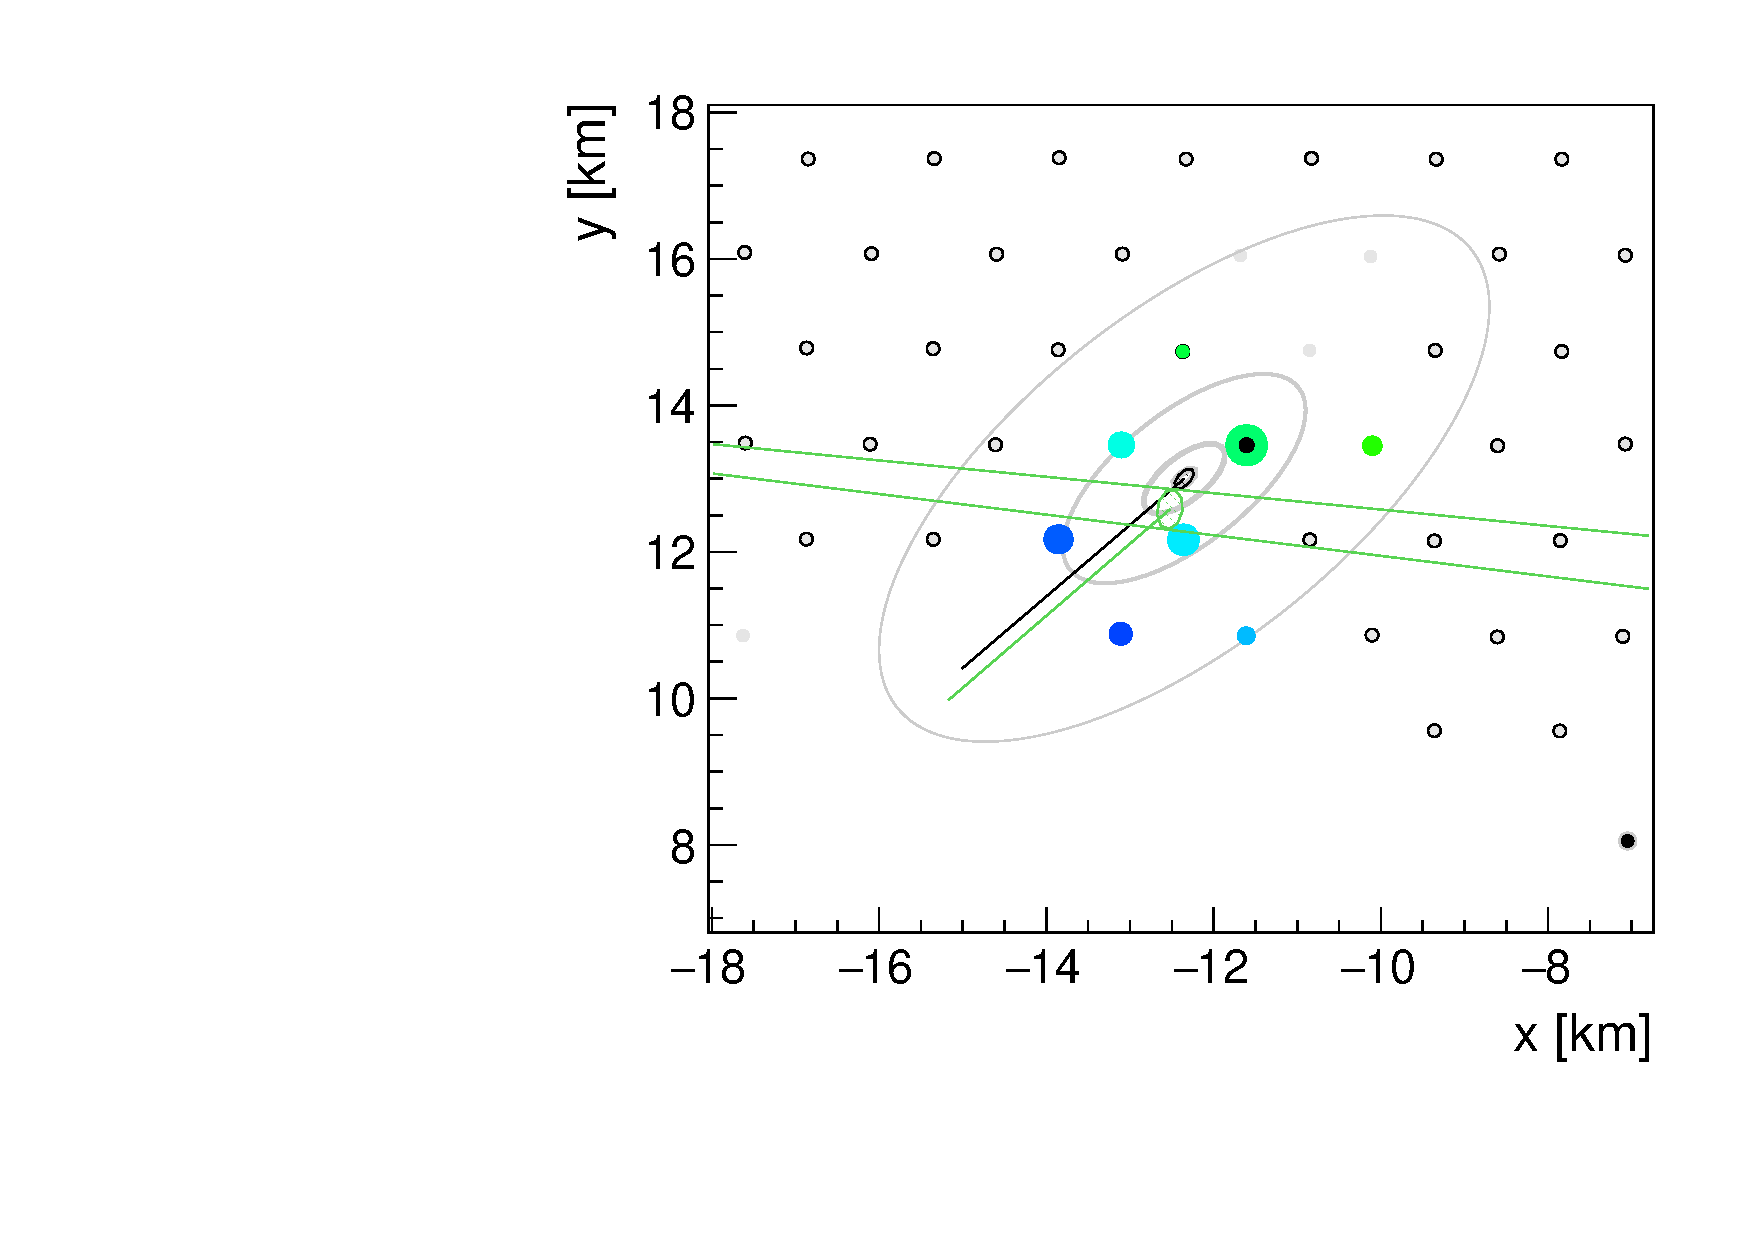
\includegraphics[width=0.8\textwidth , height=\tempheight]{/home/tsudholz/PhD/Thesis/chapters/graphs/CloudFlags/CloudCut_Events_Failed/Auger_70735278500_SdProfile.pdf}
  	\caption{SD tank triggered profile}
  \end{subfigure}

  \begin{subfigure}[b]{0.45\textwidth}
  	\centering
	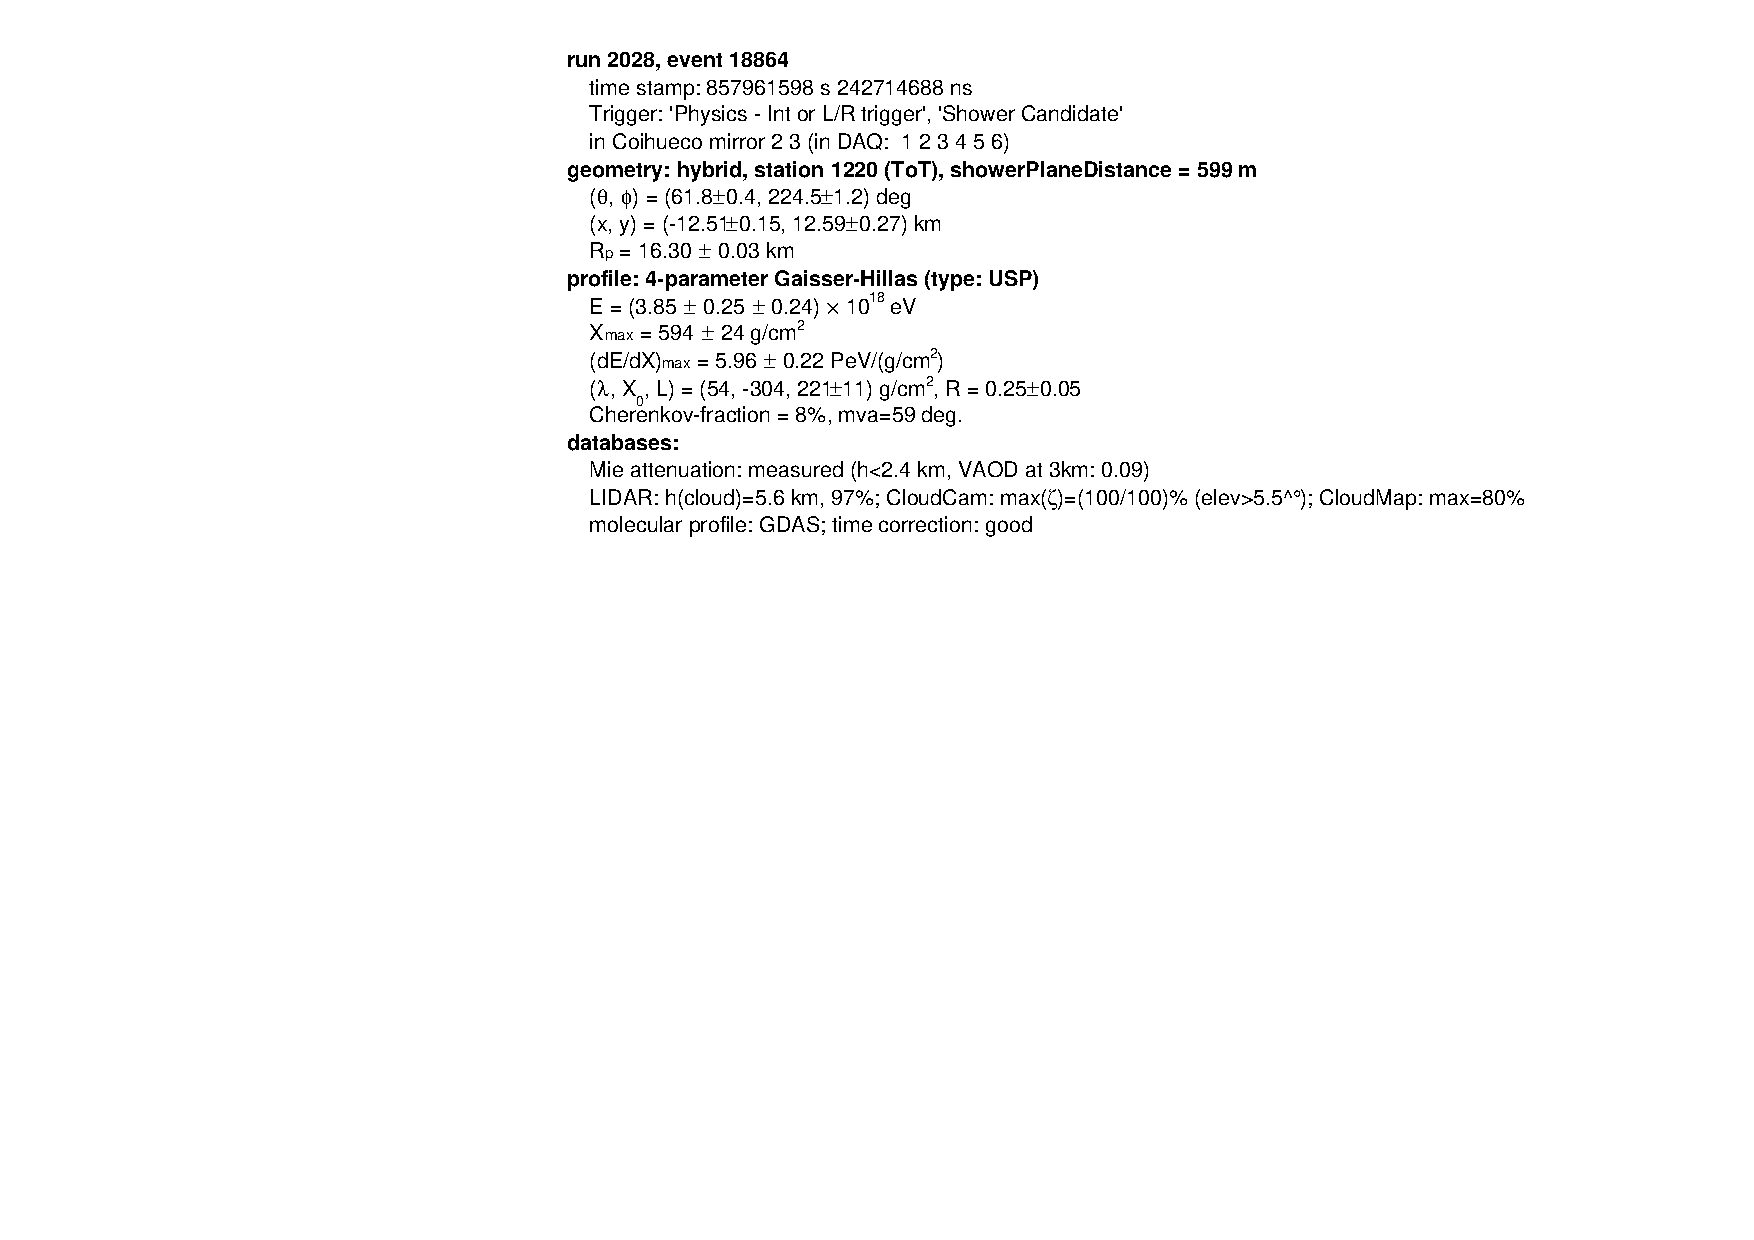
\includegraphics[height=\tempheight , trim = 0 0 5.5cm 0]{/home/tsudholz/PhD/Thesis/chapters/graphs/CloudFlags/CloudCut_Events_Failed/Auger_70735278500_FdEventInfo.pdf}
  	\caption{FD light profile}
  \end{subfigure}
  \begin{subfigure}[b]{0.45\textwidth}
  	\centering
	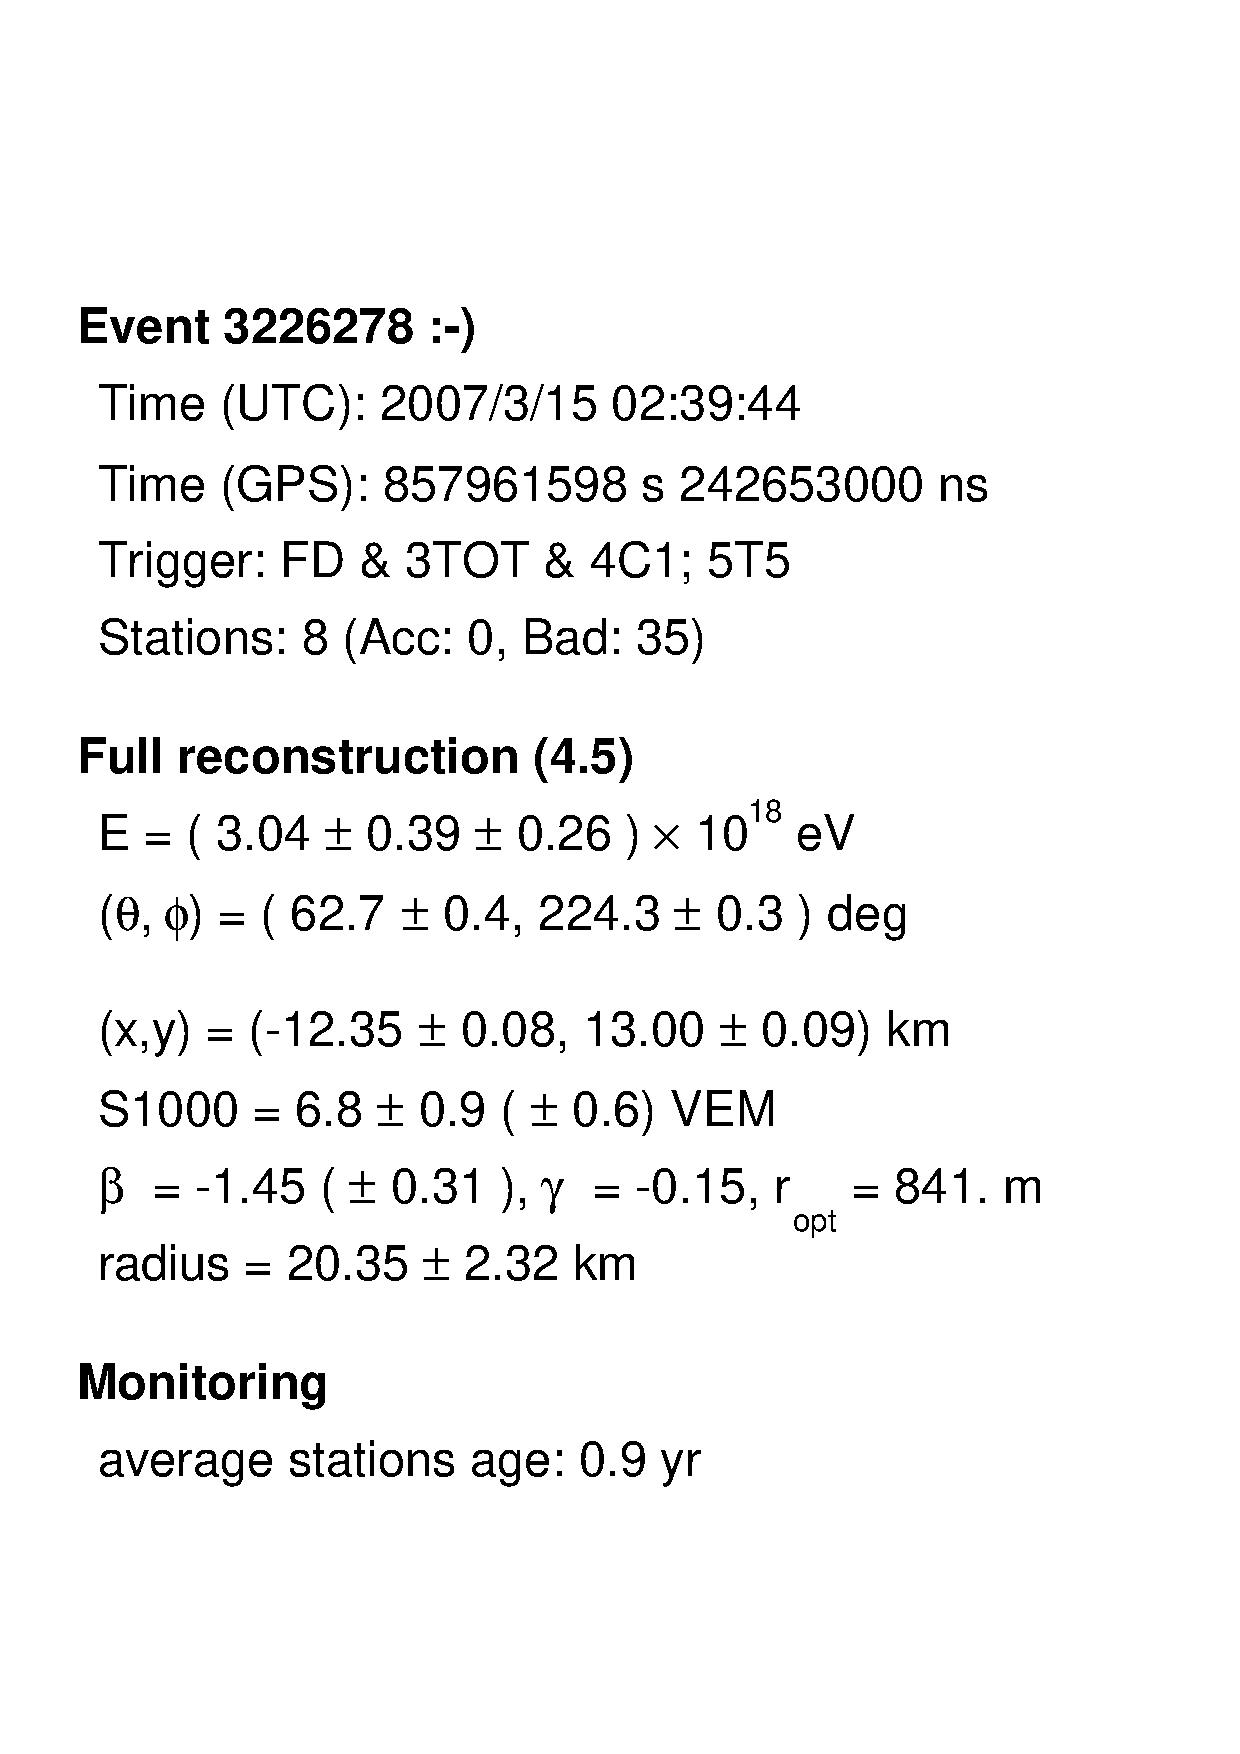
\includegraphics[height=\tempheight]{/home/tsudholz/PhD/Thesis/chapters/graphs/CloudFlags/CloudCut_Events_Failed/Auger_70735278500_SdEventInfo.pdf}
  	\caption{SD tank triggered profile}
  \end{subfigure}
  \caption{Example of an Auger event that would fail the cloud selection cut from EventBrowser}
\end{figure}

\begin{figure}
\centering
  \settoheight{\tempheight}{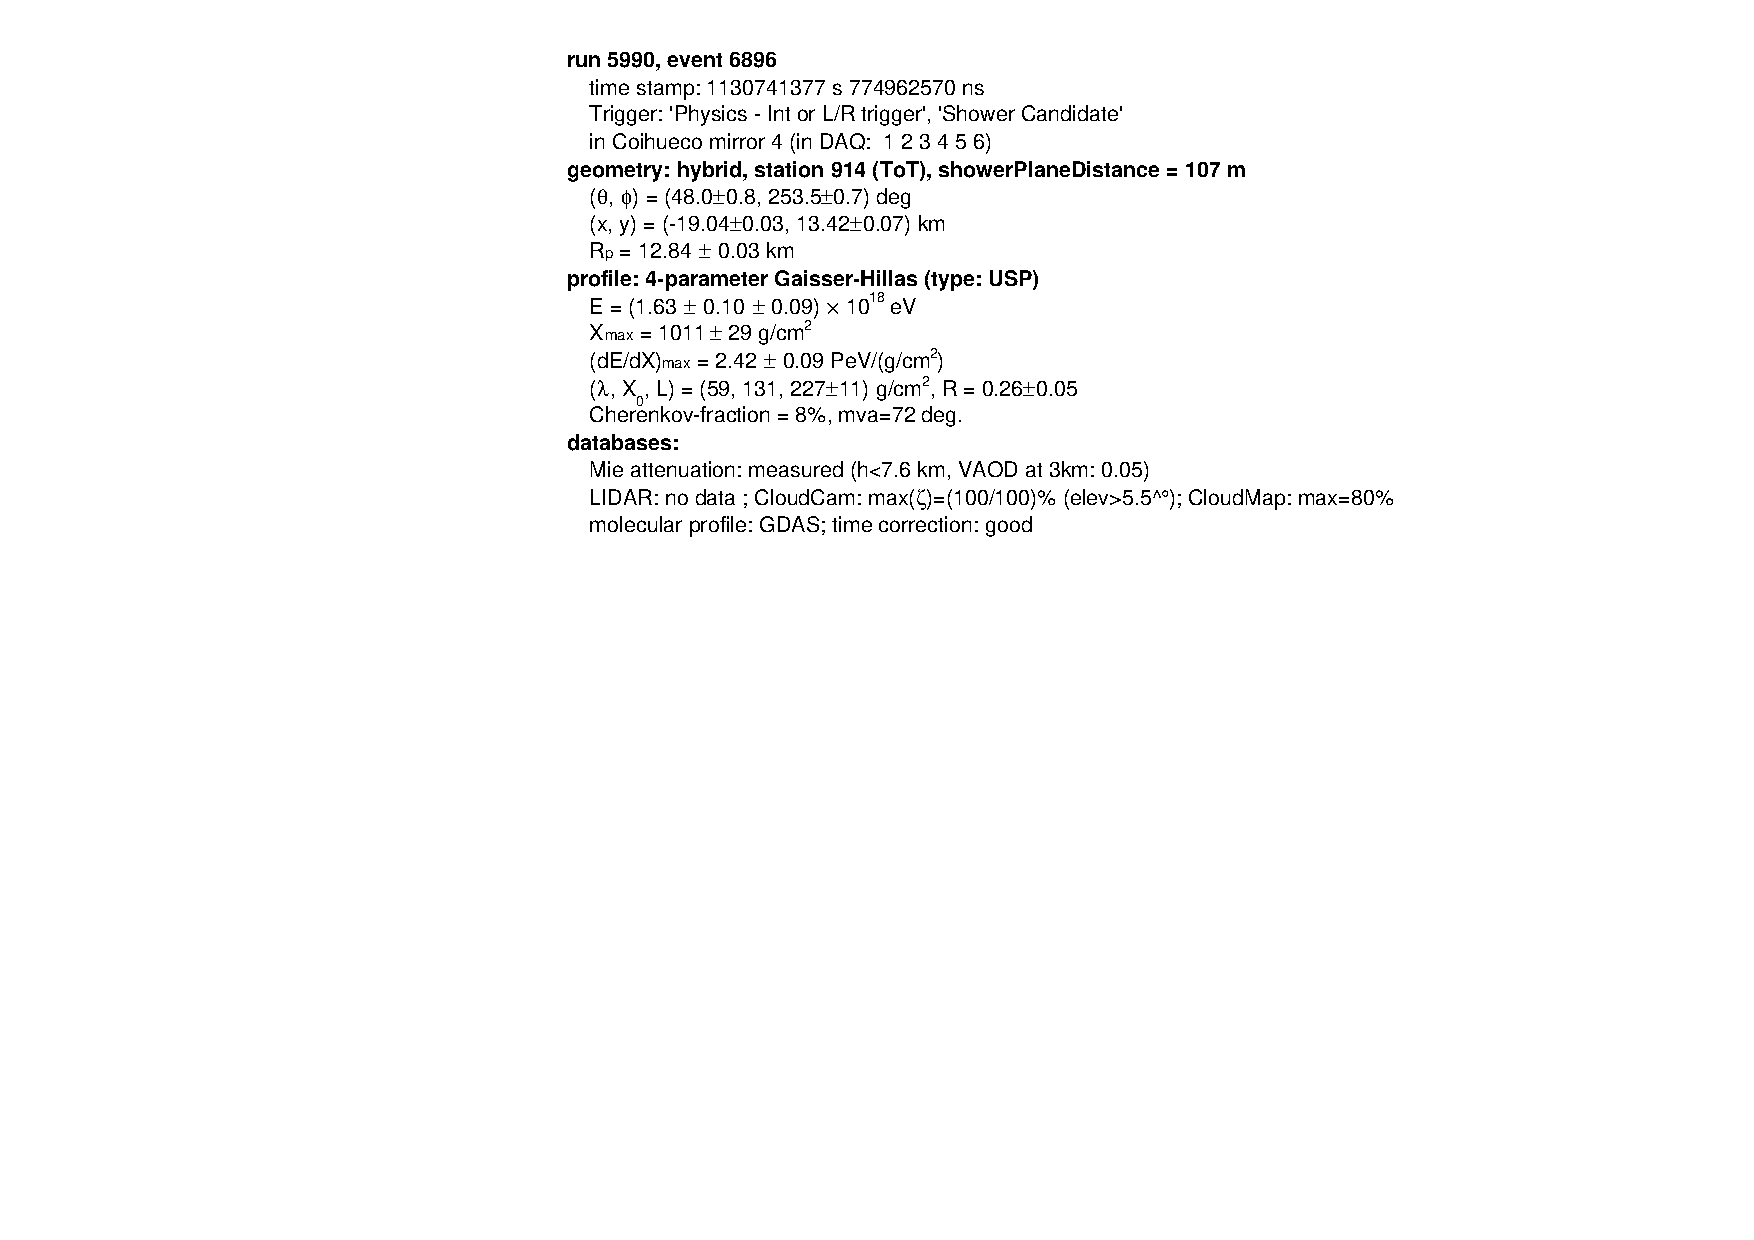
\includegraphics[width=0.45\textwidth , trim = 0 0 5.5cm 0]{/home/tsudholz/PhD/Thesis/chapters/graphs/CloudFlags/CloudCut_Events_Failed/Auger_153086776200_FdEventInfo.pdf}}
 \vspace{2cm}
  \begin{subfigure}[b]{\textwidth}
  \centering
  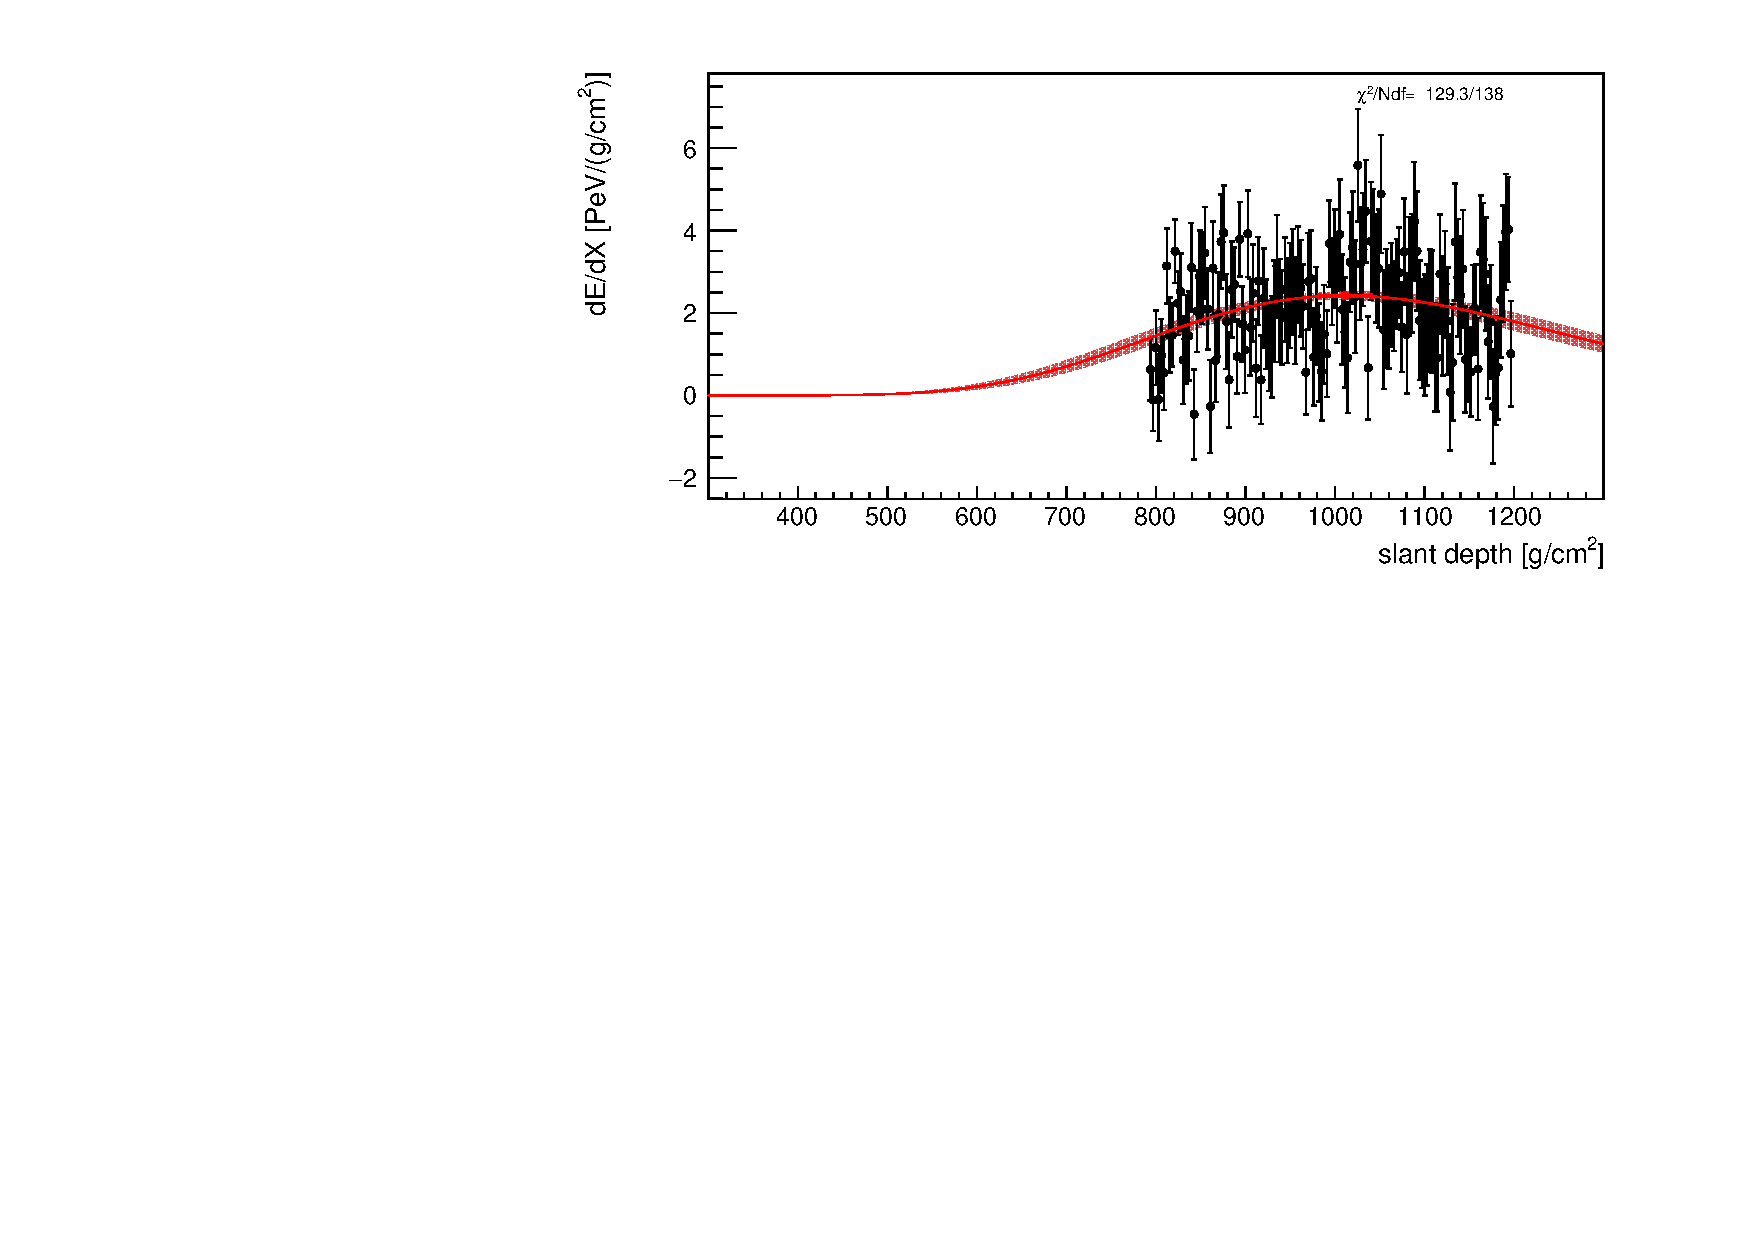
\includegraphics[width=\textwidth]{/home/tsudholz/PhD/Thesis/chapters/graphs/CloudFlags/CloudCut_Events_Failed/Auger_153086776200_SlantDepth.pdf}
  \caption{FD profile of the energy deposited as a function of atmospheric depth.}
  \end{subfigure}
 \vspace{0.5cm}
  \begin{subfigure}[b]{0.45\textwidth}
  	\centering
  	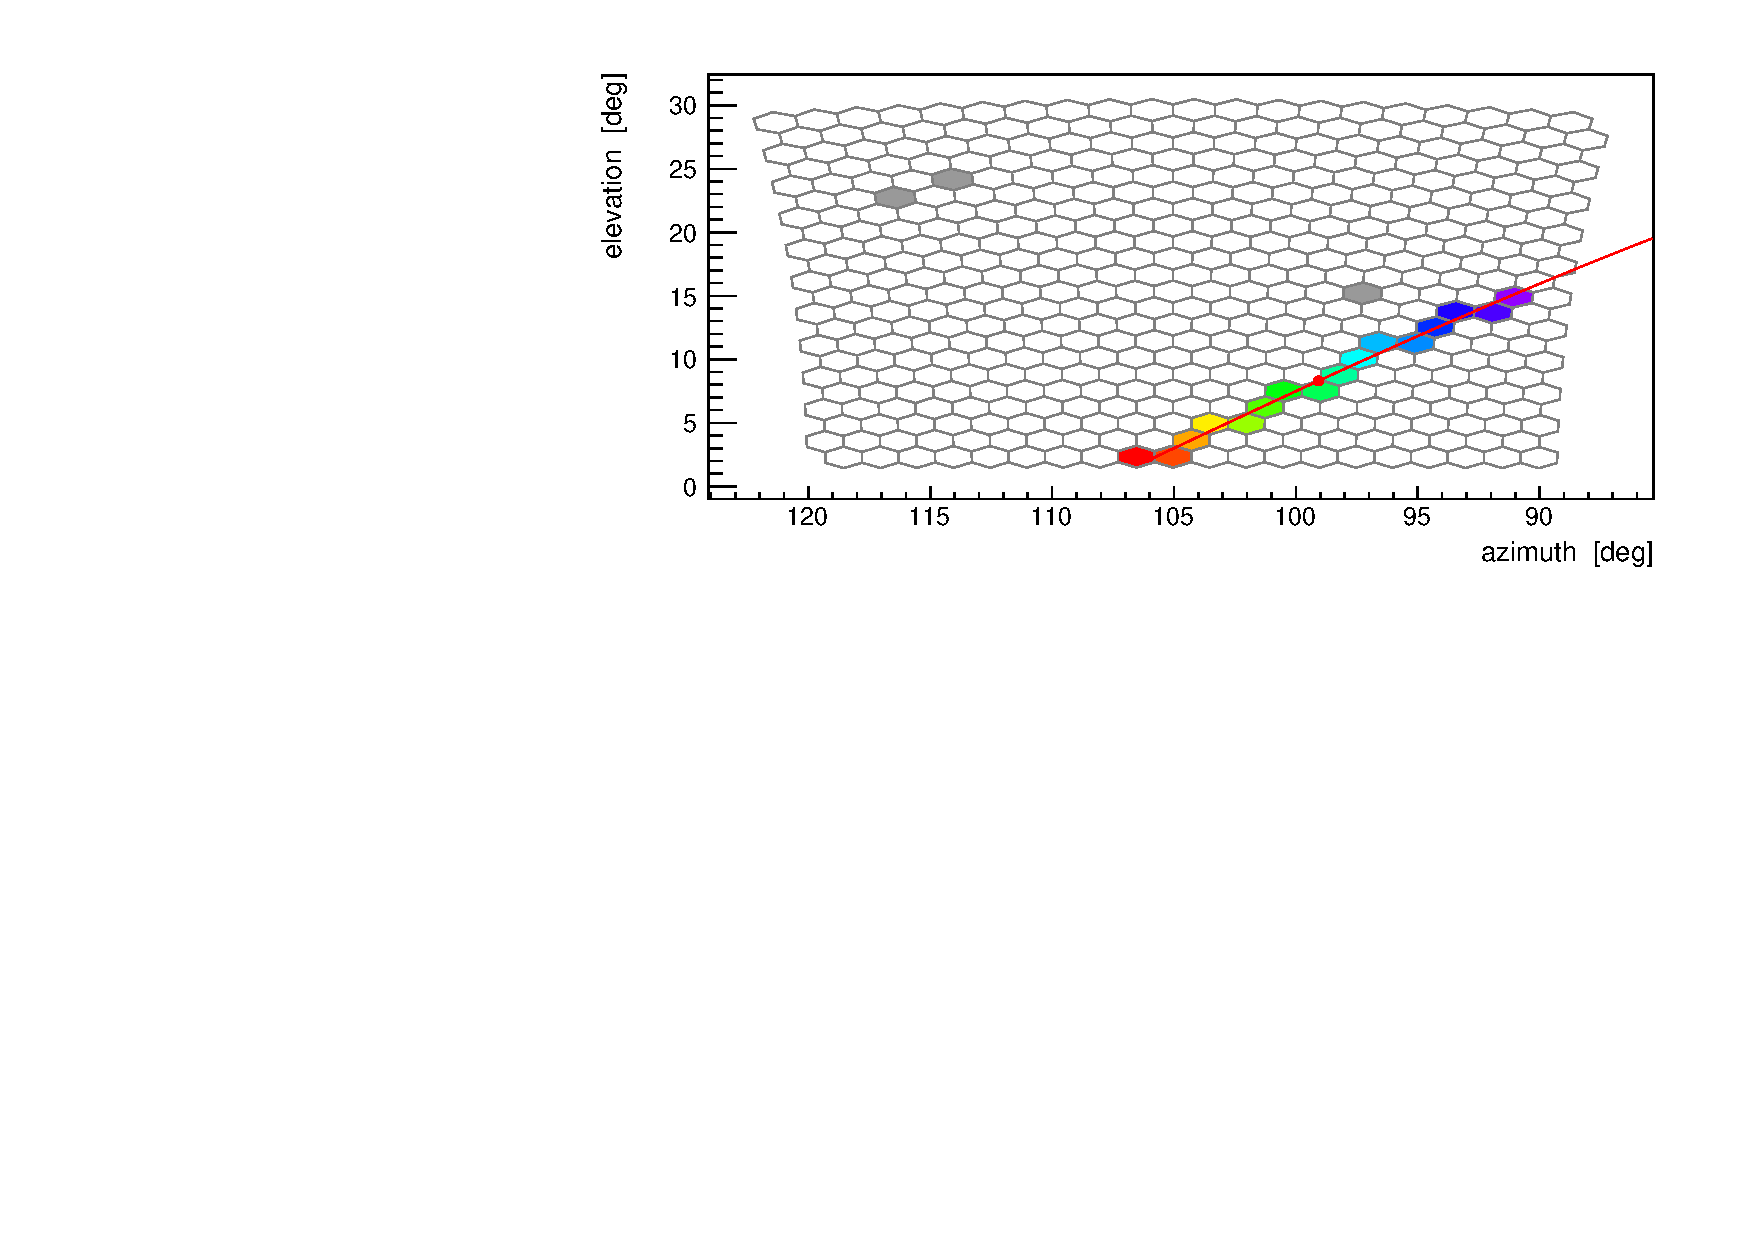
\includegraphics[width=\textwidth , height=\tempheight]{/home/tsudholz/PhD/Thesis/chapters/graphs/CloudFlags/CloudCut_Events_Failed/Auger_153086776200_FdProfile.pdf}
  	\caption{FD light profile}
  \end{subfigure}
  \begin{subfigure}[b]{0.45\textwidth}
  	\centering
  	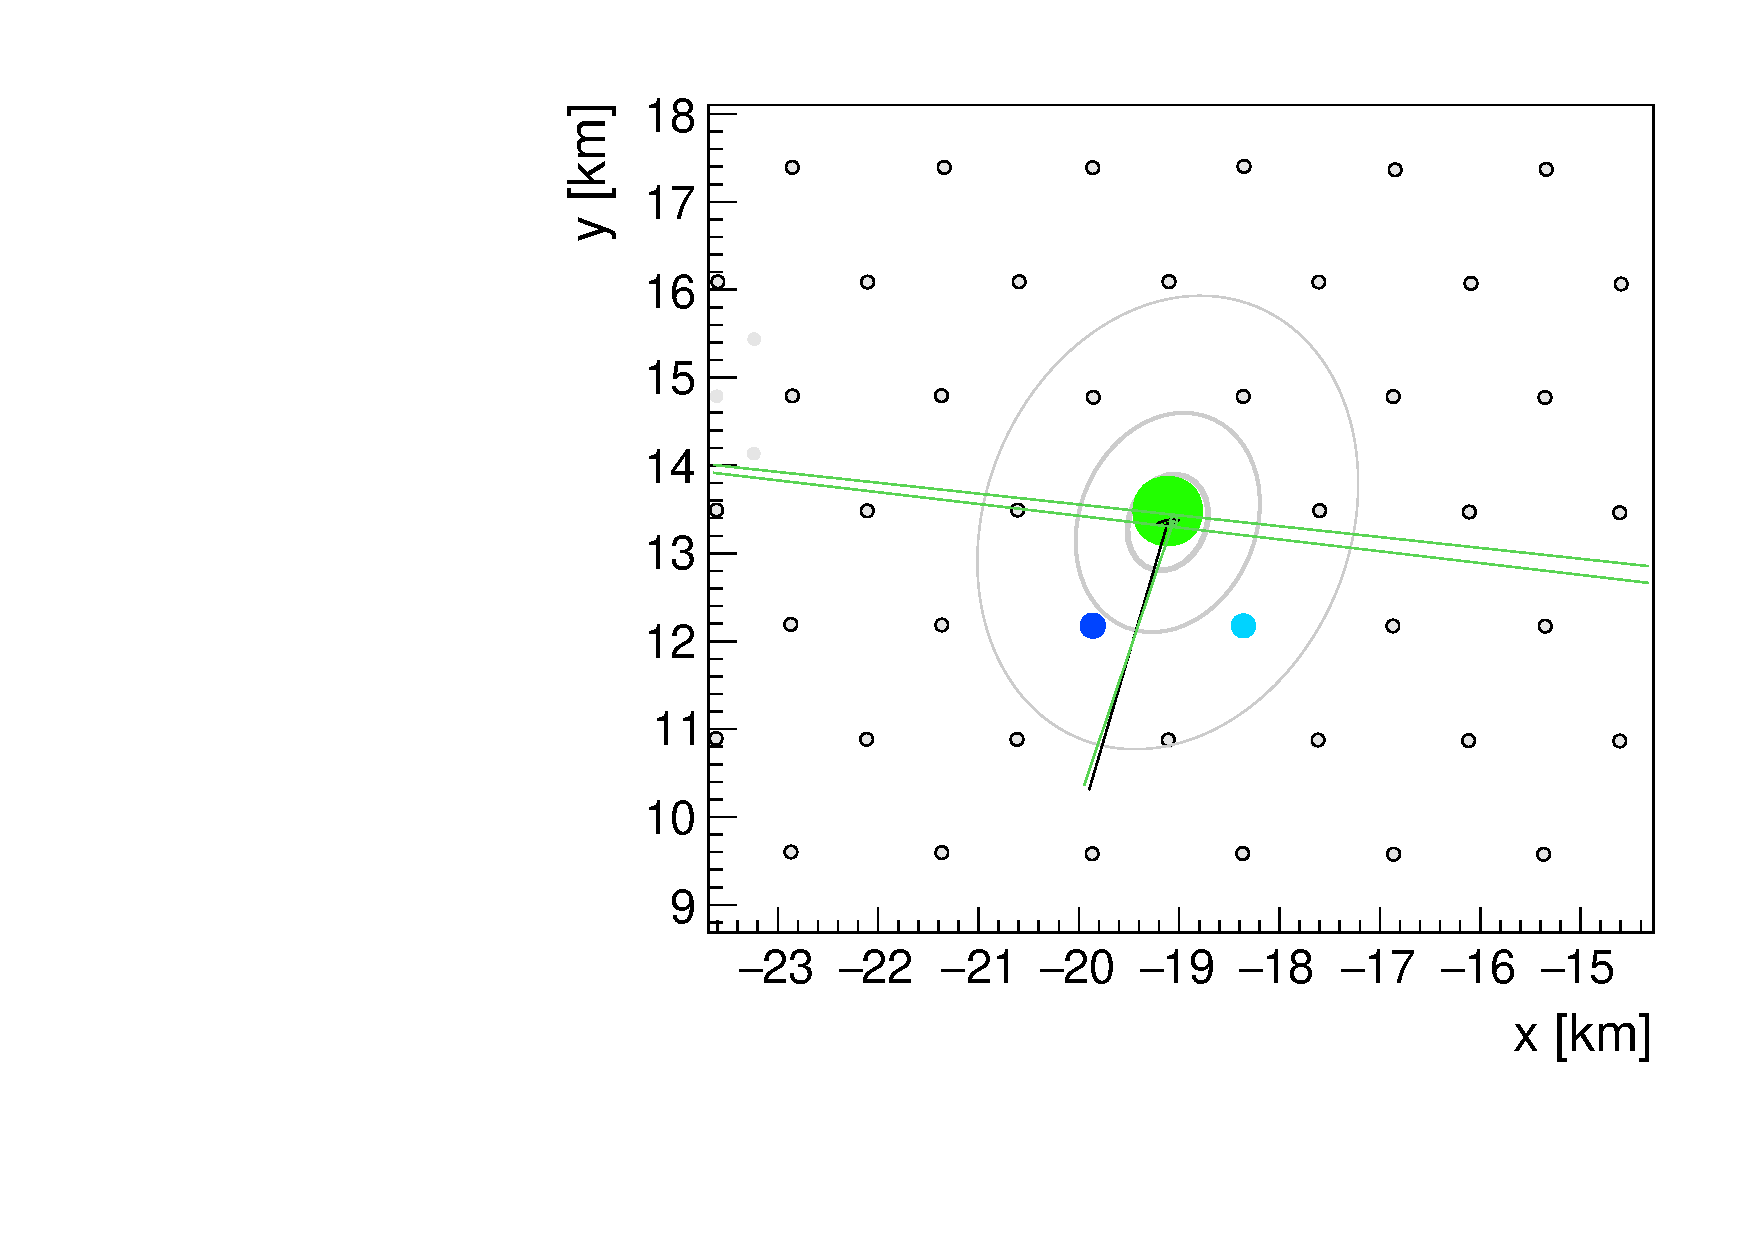
\includegraphics[width=0.8\textwidth , height=\tempheight]{/home/tsudholz/PhD/Thesis/chapters/graphs/CloudFlags/CloudCut_Events_Failed/Auger_153086776200_SdProfile.pdf}
  	\caption{SD tank triggered profile}
  \end{subfigure}

  \begin{subfigure}[b]{0.45\textwidth}
  	\centering
	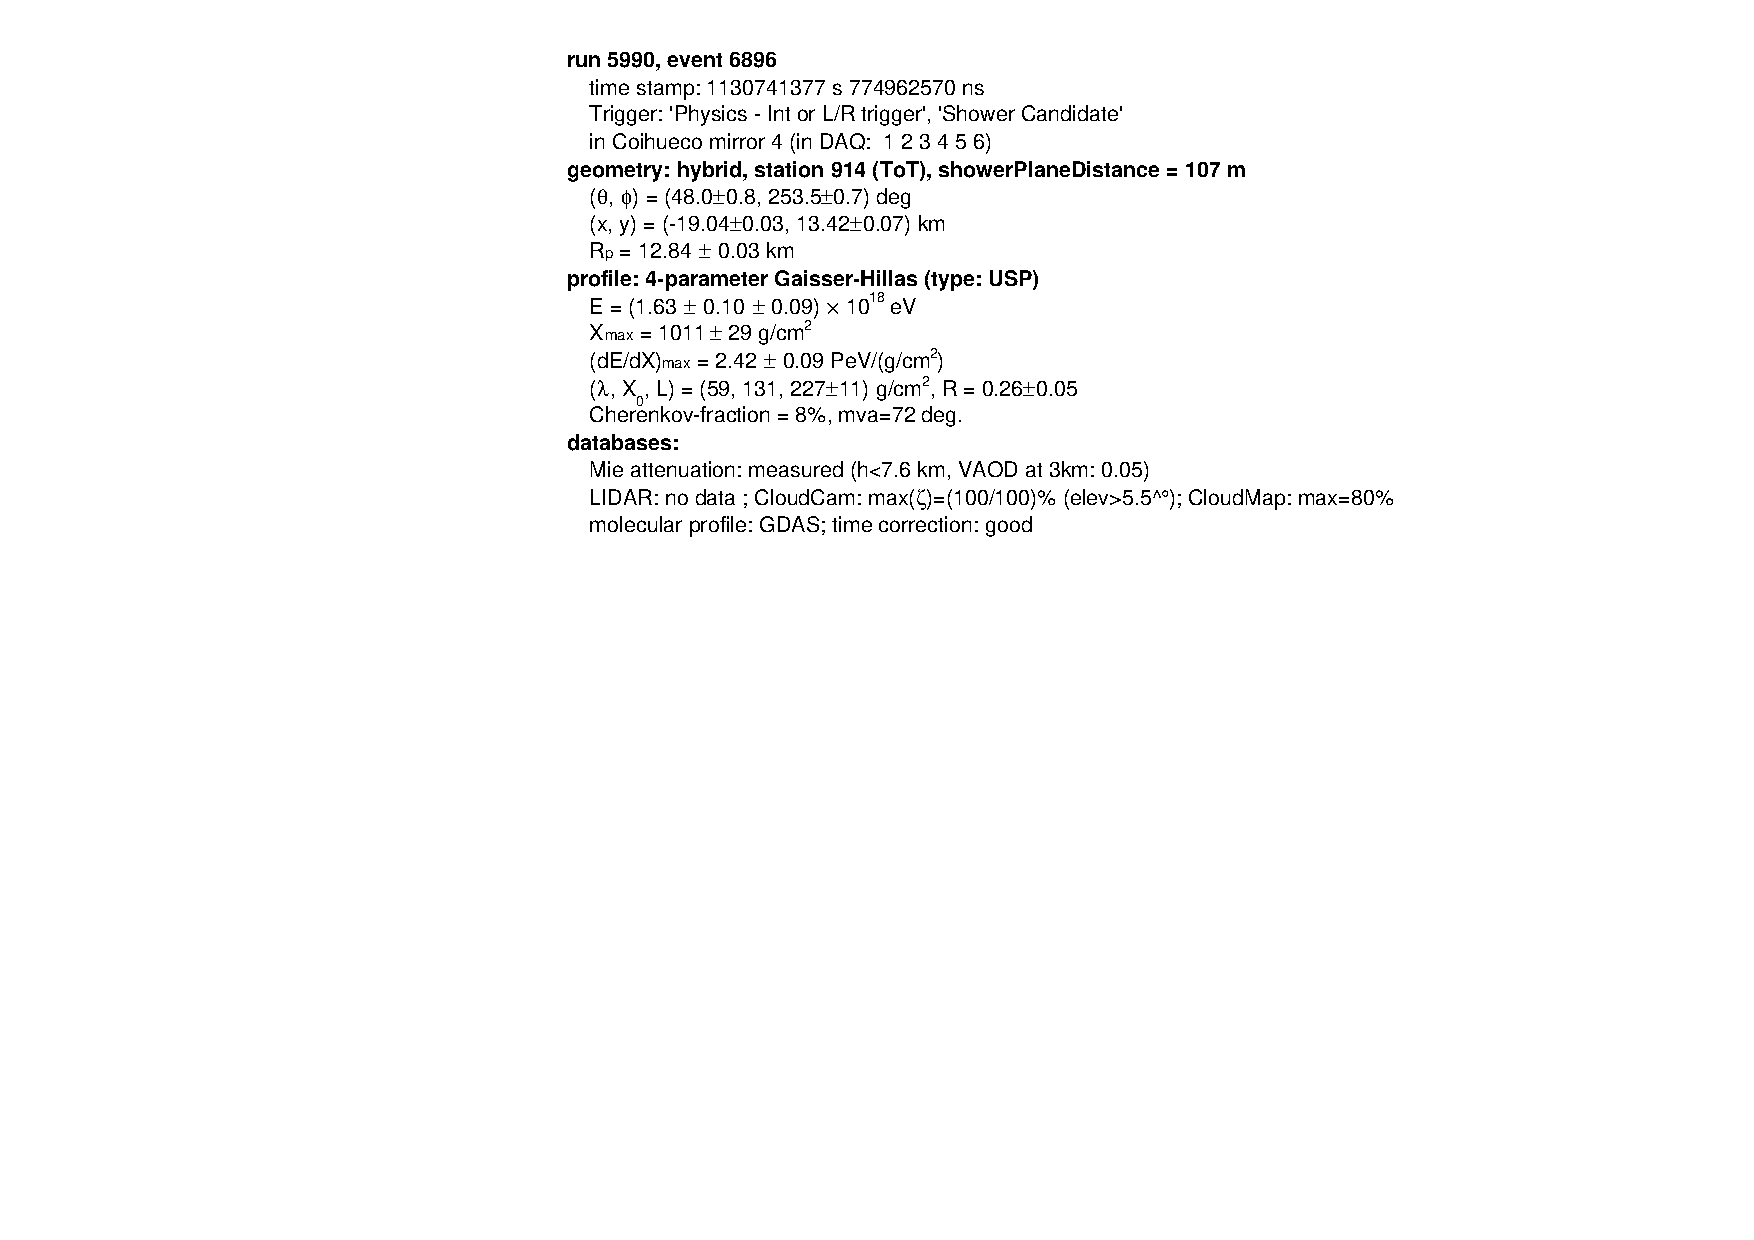
\includegraphics[height=\tempheight , trim = 0 0 5.5cm 0]{/home/tsudholz/PhD/Thesis/chapters/graphs/CloudFlags/CloudCut_Events_Failed/Auger_153086776200_FdEventInfo.pdf}
  	\caption{FD light profile}
  \end{subfigure}
  \begin{subfigure}[b]{0.45\textwidth}
  	\centering
	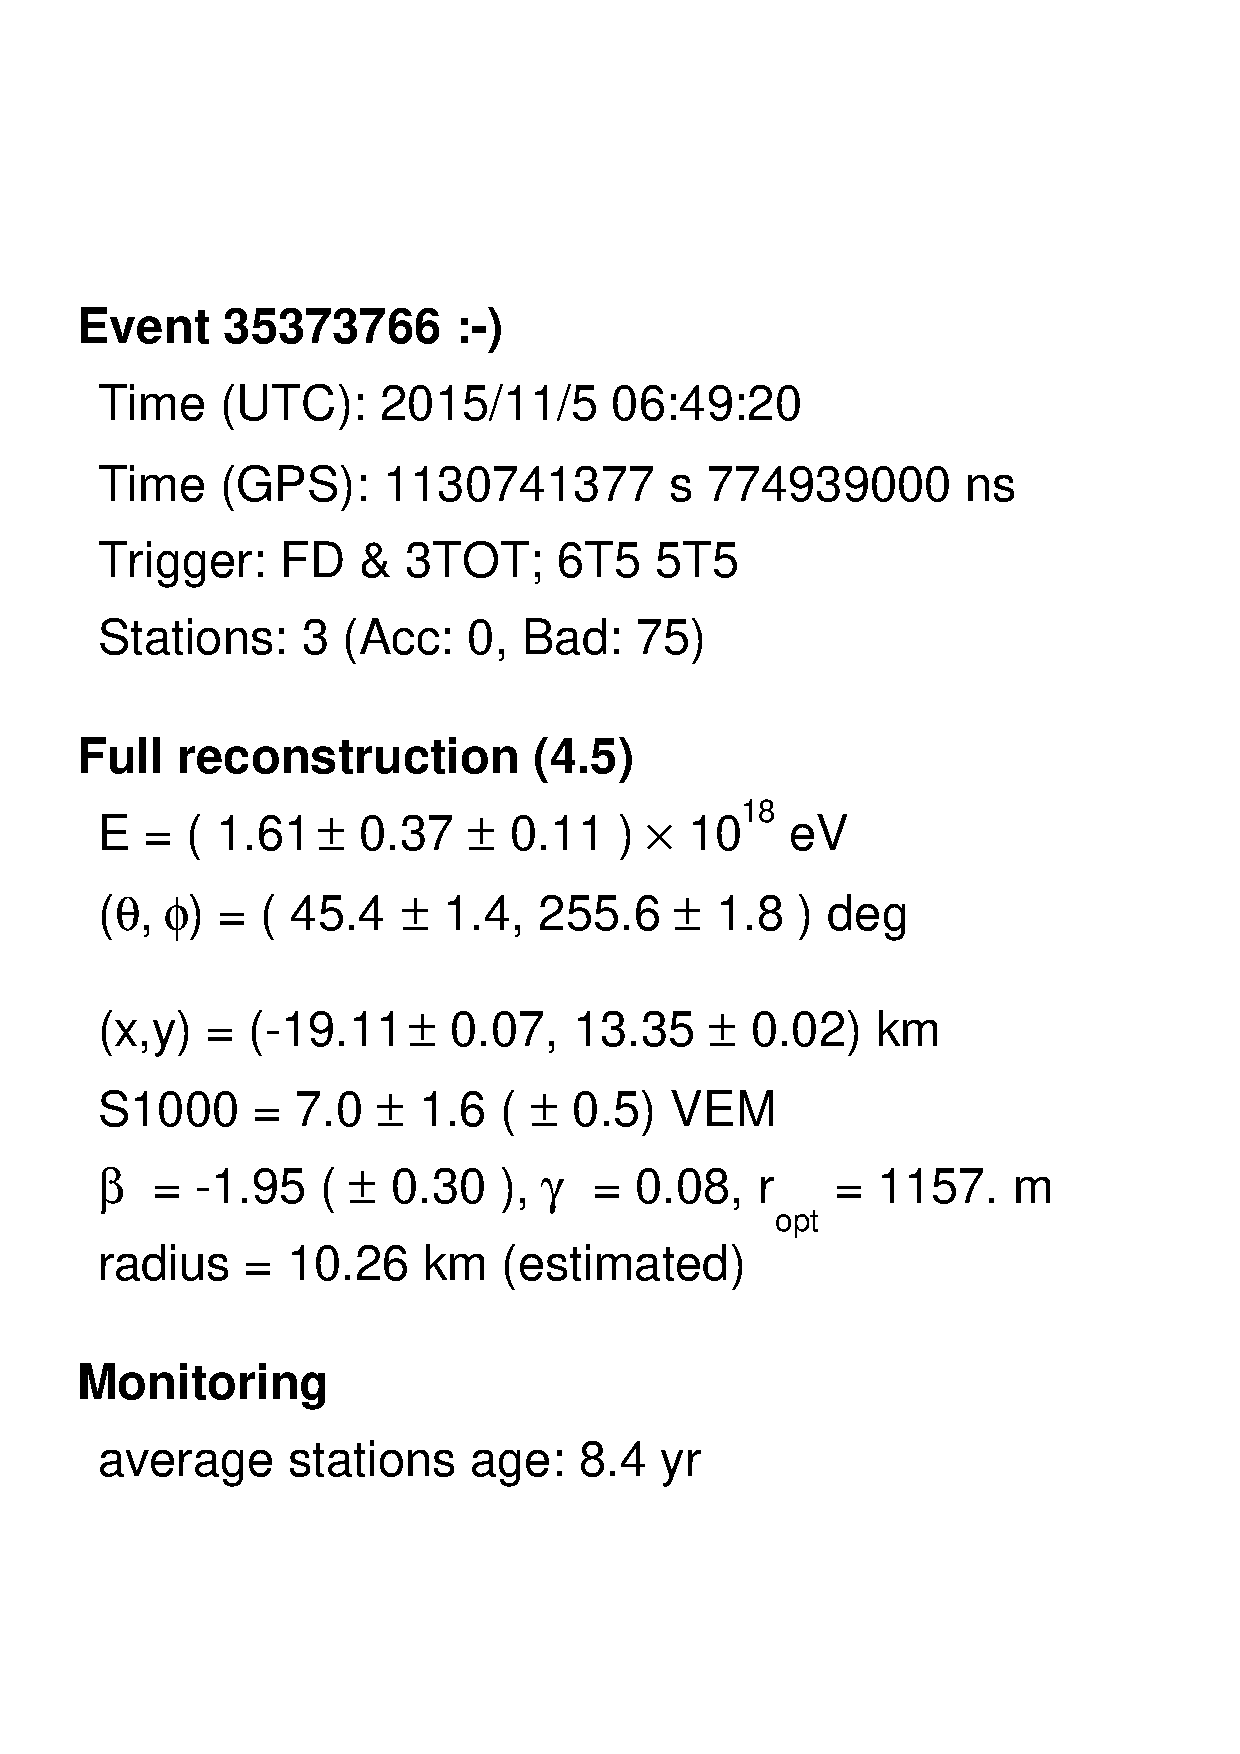
\includegraphics[height=\tempheight]{/home/tsudholz/PhD/Thesis/chapters/graphs/CloudFlags/CloudCut_Events_Failed/Auger_153086776200_SdEventInfo.pdf}
  	\caption{SD tank triggered profile}
  \end{subfigure}
  \caption{Example of an Auger event that would fail the cloud selection cut from EventBrowser}
\end{figure}

\subsection{Examples of Events that have passed Cloud Selection Cuts from EventBrowser}

% Events that would fail the cloud cut only

\begin{figure}
\centering
  \settoheight{\tempheight}{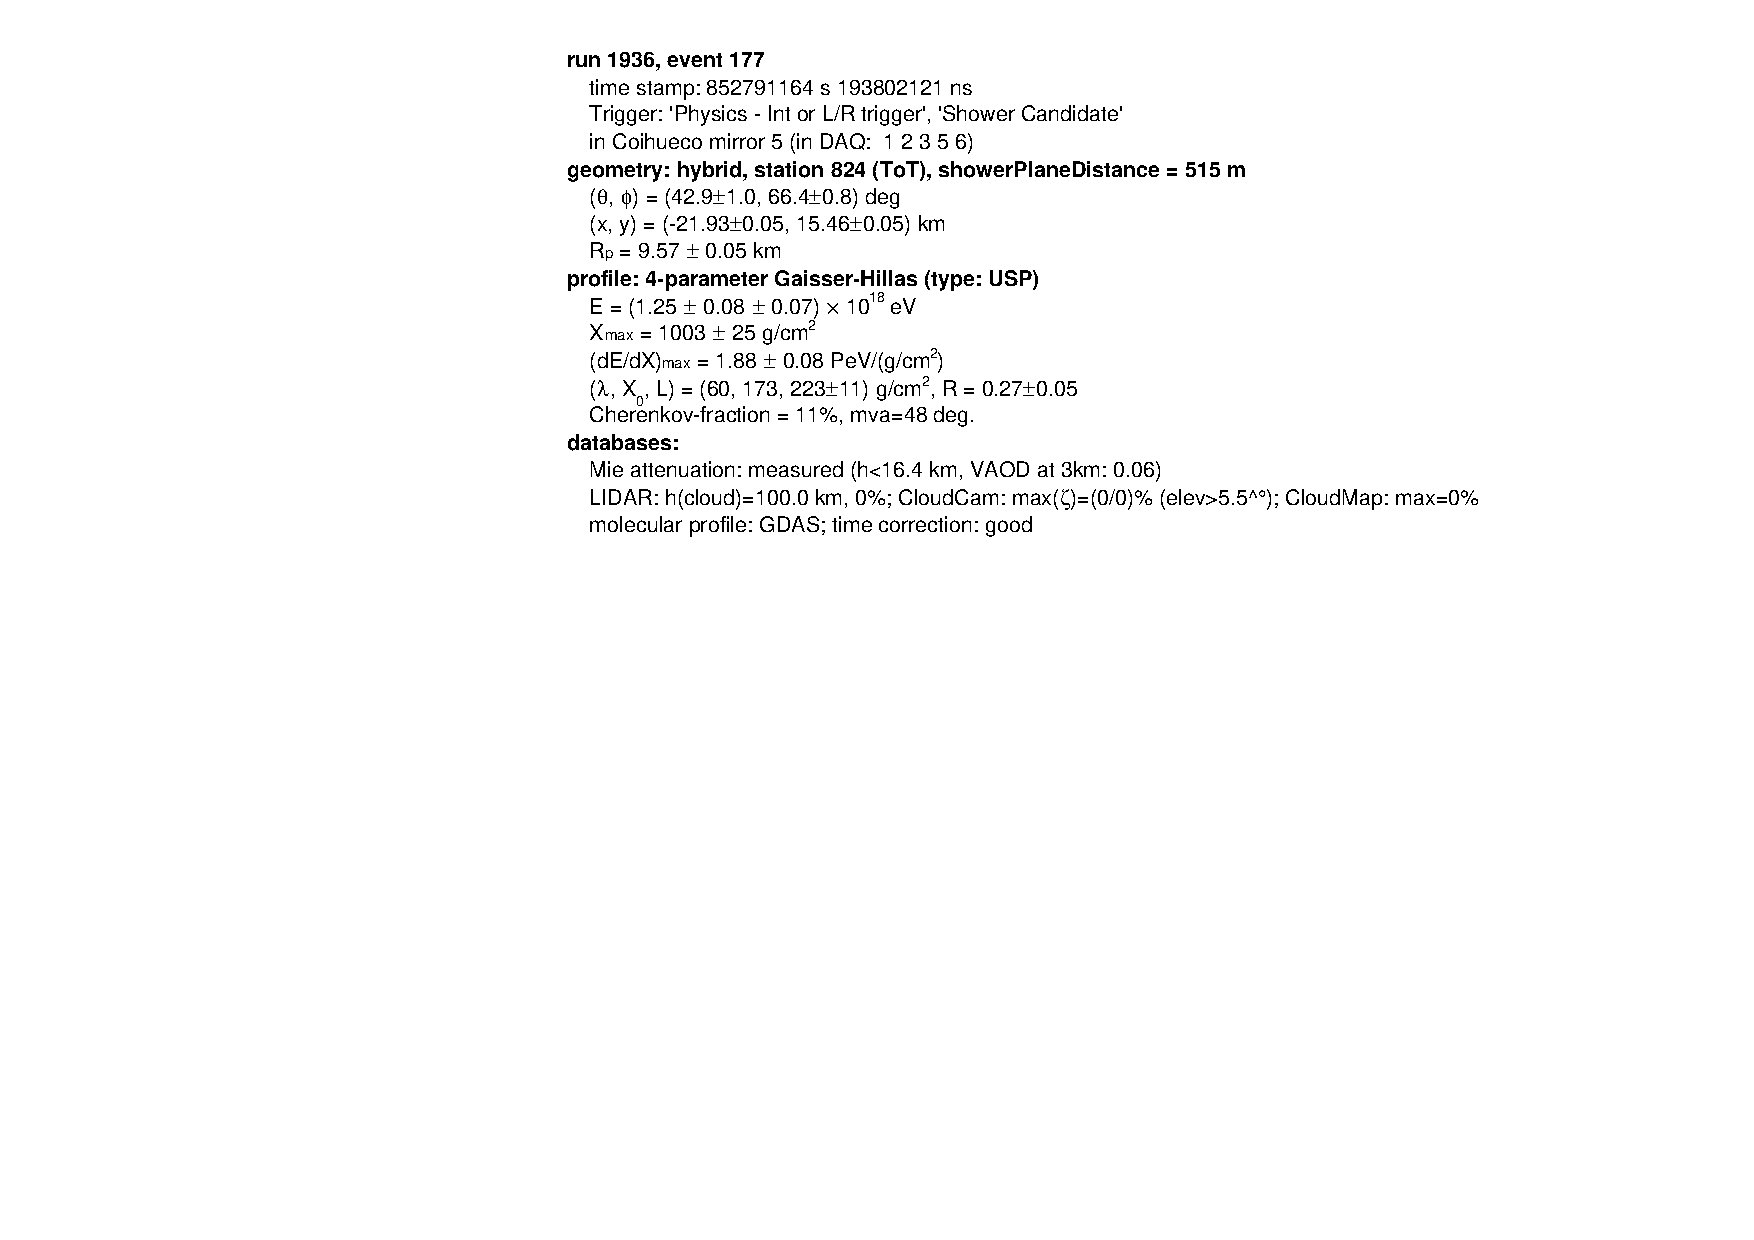
\includegraphics[width=0.45\textwidth , trim = 0 0 5.5cm 0]{/home/tsudholz/PhD/Thesis/chapters/graphs/CloudFlags/CloudCut_Events/Auger_70136635100_FdEventInfo.pdf}}
 \vspace{2cm}
  \begin{subfigure}[b]{\textwidth}
  \centering
  \includegraphics[width=\textwidth]{/home/tsudholz/PhD/Thesis/chapters/graphs/CloudFlags/CloudCut_Events/Auger_70136635100_SlantDepth.pdf}
  \caption{FD profile of the energy deposited as a function of atmospheric depth.}
  \end{subfigure}
 \vspace{0.5cm}
  \begin{subfigure}[b]{0.45\textwidth}
  	\centering
  	\includegraphics[width=\textwidth , height=\tempheight]{/home/tsudholz/PhD/Thesis/chapters/graphs/CloudFlags/CloudCut_Events/Auger_70136635100_FdProfile.pdf}
  	\caption{FD light profile}
  \end{subfigure}
  \begin{subfigure}[b]{0.45\textwidth}
  	\centering
  	\includegraphics[width=0.8\textwidth , height=\tempheight]{/home/tsudholz/PhD/Thesis/chapters/graphs/CloudFlags/CloudCut_Events/Auger_70136635100_SdProfile.pdf}
  	\caption{SD tank triggered profile}
  \end{subfigure}

  \begin{subfigure}[b]{0.45\textwidth}
  	\centering
	\includegraphics[height=\tempheight , trim = 0 0 5.5cm 0]{/home/tsudholz/PhD/Thesis/chapters/graphs/CloudFlags/CloudCut_Events/Auger_70136635100_FdEventInfo.pdf}
  	\caption{FD light profile}
  \end{subfigure}
  \begin{subfigure}[b]{0.45\textwidth}
  	\centering
	\includegraphics[height=\tempheight]{/home/tsudholz/PhD/Thesis/chapters/graphs/CloudFlags/CloudCut_Events/Auger_70136635100_SdEventInfo.pdf}
  	\caption{SD tank triggered profile}
  \end{subfigure}
  \caption{Example of an Auger event that would pass the cloud selection cut from EventBrowser}
\end{figure}

\begin{figure}
\centering
  \settoheight{\tempheight}{\includegraphics[width=0.45\textwidth , trim = 0 0 5.5cm 0]{/home/tsudholz/PhD/Thesis/chapters/graphs/CloudFlags/CloudCut_Events/Auger_101576030600_FdEventInfo.pdf}}
 \vspace{2cm}
  \begin{subfigure}[b]{\textwidth}
  \centering
  \includegraphics[width=\textwidth]{/home/tsudholz/PhD/Thesis/chapters/graphs/CloudFlags/CloudCut_Events/Auger_101576030600_SlantDepth.pdf}
  \caption{FD profile of the energy deposited as a function of atmospheric depth.}
  \end{subfigure}
 \vspace{0.5cm}
  \begin{subfigure}[b]{0.45\textwidth}
  	\centering
  	\includegraphics[width=\textwidth , height=\tempheight]{/home/tsudholz/PhD/Thesis/chapters/graphs/CloudFlags/CloudCut_Events/Auger_101576030600_FdProfile.pdf}
  	\caption{FD light profile}
  \end{subfigure}
  \begin{subfigure}[b]{0.45\textwidth}
  	\centering
  	\includegraphics[width=0.8\textwidth , height=\tempheight]{/home/tsudholz/PhD/Thesis/chapters/graphs/CloudFlags/CloudCut_Events/Auger_101576030600_SdProfile.pdf}
  	\caption{SD tank triggered profile}
  \end{subfigure}

  \begin{subfigure}[b]{0.45\textwidth}
  	\centering
	\includegraphics[height=\tempheight , trim = 0 0 5.5cm 0]{/home/tsudholz/PhD/Thesis/chapters/graphs/CloudFlags/CloudCut_Events/Auger_101576030600_FdEventInfo.pdf}
  	\caption{FD light profile}
  \end{subfigure}
  \begin{subfigure}[b]{0.45\textwidth}
  	\centering
	\includegraphics[height=\tempheight]{/home/tsudholz/PhD/Thesis/chapters/graphs/CloudFlags/CloudCut_Events/Auger_101576030600_SdEventInfo.pdf}
  	\caption{SD tank triggered profile}
  \end{subfigure}
  \caption{Example of an Auger event that would pass the cloud selection cut from EventBrowser}
\end{figure}

\begin{figure}
\centering
  \settoheight{\tempheight}{\includegraphics[width=0.45\textwidth , trim = 0 0 5.5cm 0]{/home/tsudholz/PhD/Thesis/chapters/graphs/CloudFlags/CloudCut_Events/Auger_92285877600_FdEventInfo.pdf}}
 \vspace{2cm}
  \begin{subfigure}[b]{\textwidth}
  \centering
  \includegraphics[width=\textwidth]{/home/tsudholz/PhD/Thesis/chapters/graphs/CloudFlags/CloudCut_Events/Auger_92285877600_SlantDepth.pdf}
  \caption{FD profile of the energy deposited as a function of atmospheric depth.}
  \end{subfigure}
 \vspace{0.5cm}
  \begin{subfigure}[b]{0.45\textwidth}
  	\centering
  	\includegraphics[width=\textwidth , height=\tempheight]{/home/tsudholz/PhD/Thesis/chapters/graphs/CloudFlags/CloudCut_Events/Auger_92285877600_FdProfile.pdf}
  	\caption{FD light profile}
  \end{subfigure}
  \begin{subfigure}[b]{0.45\textwidth}
  	\centering
  	\includegraphics[width=0.8\textwidth , height=\tempheight]{/home/tsudholz/PhD/Thesis/chapters/graphs/CloudFlags/CloudCut_Events/Auger_92285877600_SdProfile.pdf}
  	\caption{SD tank triggered profile}
  \end{subfigure}

  \begin{subfigure}[b]{0.45\textwidth}
  	\centering
	\includegraphics[height=\tempheight , trim = 0 0 5.5cm 0]{/home/tsudholz/PhD/Thesis/chapters/graphs/CloudFlags/CloudCut_Events/Auger_92285877600_FdEventInfo.pdf}
  	\caption{FD light profile}
  \end{subfigure}
  \begin{subfigure}[b]{0.45\textwidth}
  	\centering
	\includegraphics[height=\tempheight]{/home/tsudholz/PhD/Thesis/chapters/graphs/CloudFlags/CloudCut_Events/Auger_92285877600_SdEventInfo.pdf}
  	\caption{SD tank triggered profile}
  \end{subfigure}
  \caption{Example of an Auger event that would pass the cloud selection cut from EventBrowser}
\end{figure}

\section{Discussion - Are we being too conservative?}

Gaining 30\% more events cut is removed

Have to be careful of outliers

Mean Xmax and spread in Xmax does not change significantly

With cloud cut confident that events that could be cloud effected are removed. Without the cloud cut no significant impact is seem expect for the increase of statistics by 30\%.


\section{Conclusion}
